%% main text
\section{Introduction}
\label{S:intro}

The standard model predicts that the top quark, like other massive fermions,  acquires its mass, $m_\mathrm{t}$, through its Yukawa coupling to the Higgs field, $g_\mathrm{t}=m_\mathrm{t}/\sqrt{2}v$, where $v$ is the vacuum expectation value of the Higgs field. Among all such couplings, the top quark Yukawa coupling  is of particular interest. It is not only the largest, but also suspiciously close to unity. This makes the coupling both theoretically intriguing and experimentally accessible to measurement. Recent efforts have seen the first success in directly constraining $g_\mathrm{t}$ \cite{ttH}. However, it is also possible to constrain $g_\mathrm{t}$ indirectly using the kinematic distributions of top and antitop quarks produced in hadronic collisions, as done recently in \cite{ytpaper}. This analysis follows closely the latter approach, which we will briefly outline, and adapts it to a different \ttbar decay channel.

Current Monte Carlo (MC) simulations of \ttbar production include next-to-leading order (NLO) precision in perturbative Quantum Chromodynamics (QCD). Sub-leading-order corrections arise from including electroweak (EW) terms in a perturbative expansion of $\alpha_S$ and $\alpha_\mathrm{EW}$, the latter of which is much smaller and traditionally shortened to $\alpha$. Such terms begin to noticeably affect the cross-section only at loop-induced order $\alpha_s^2 \alpha$, and are typically ignored. While these have a very small effect on the total cross-section, they can alter the shape of kinematic distributions to a measurable extent. Such changes will be more noticeable if the Yukawa coupling affecting the loop correction (Figure \ref{fig:diagrams}) is anomalously large. Thus, these corrections are of particular interest in placing upper limits on $g_t$. For example, the distribution of the invariant mass of the \ttbar system, $M_{\ttb}$, will be affected significantly by varying $g_\mathrm{t}$. In particular, doubling the value of $g_\mathrm{t}$ can alter the $M_{\ttb}$ distribution by about 9\% near the production threshold as described in \cite{Uwer} and shown in Figure \ref{fig:hatratgen}(left). Another variable sensitive to the value of $g_\mathrm{t}$ is the difference in rapidity between top and anti top quarks $\Delta y_{\ttb} = y(\mathrm{t})-y(\mathrm{\bar{t})}$ , shown in Figure \ref{fig:hatratgen}(right). Together, these two variables form a basis for a 2D differential cross section of \ttbar decays, and can be used to include the EW corrections on arbitrary samples via weights.
\begin{figure}
    \centering
    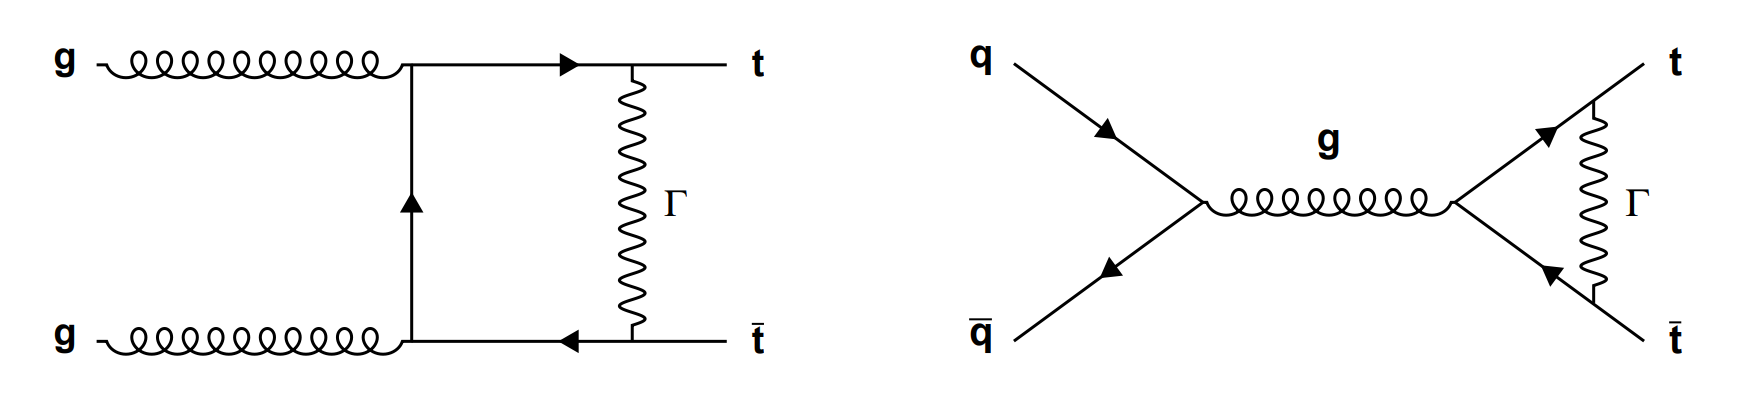
\includegraphics[width=.85\linewidth]{figs/quarkgluon.png}
    \caption{Sample diagrams for EW contributions to gluon-induced and quark-induced top pair production, where $\Gamma$ stands for neutral gauge bosons, Higgs boson and pseudo-Goldstone bosons. The correction due to the interference of these diagrams with the LO QCD diagrams is evaluated using HATHOR package}.
    \label{fig:diagrams}
\end{figure}

\begin{figure}
    \centering
    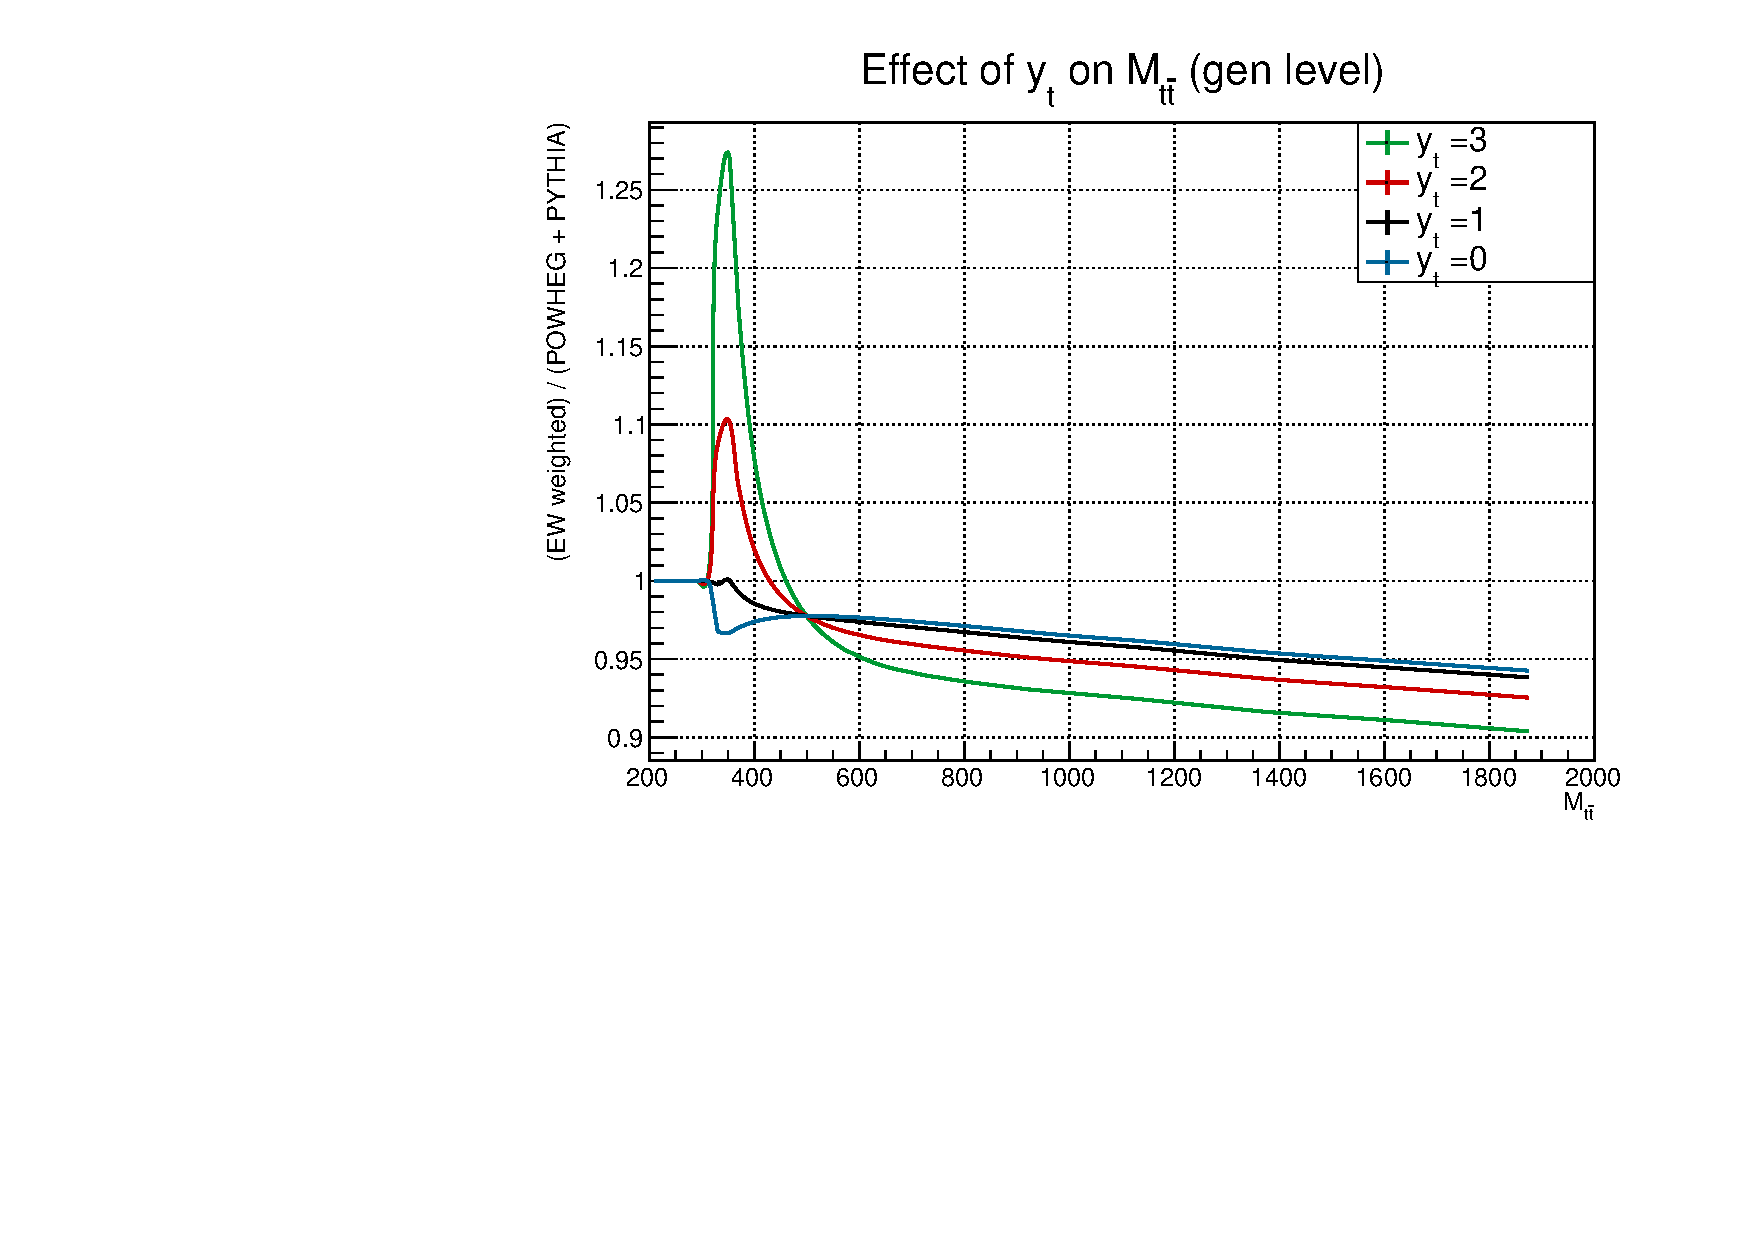
\includegraphics[width=.48\linewidth]{figs/ratMttgen.pdf}
    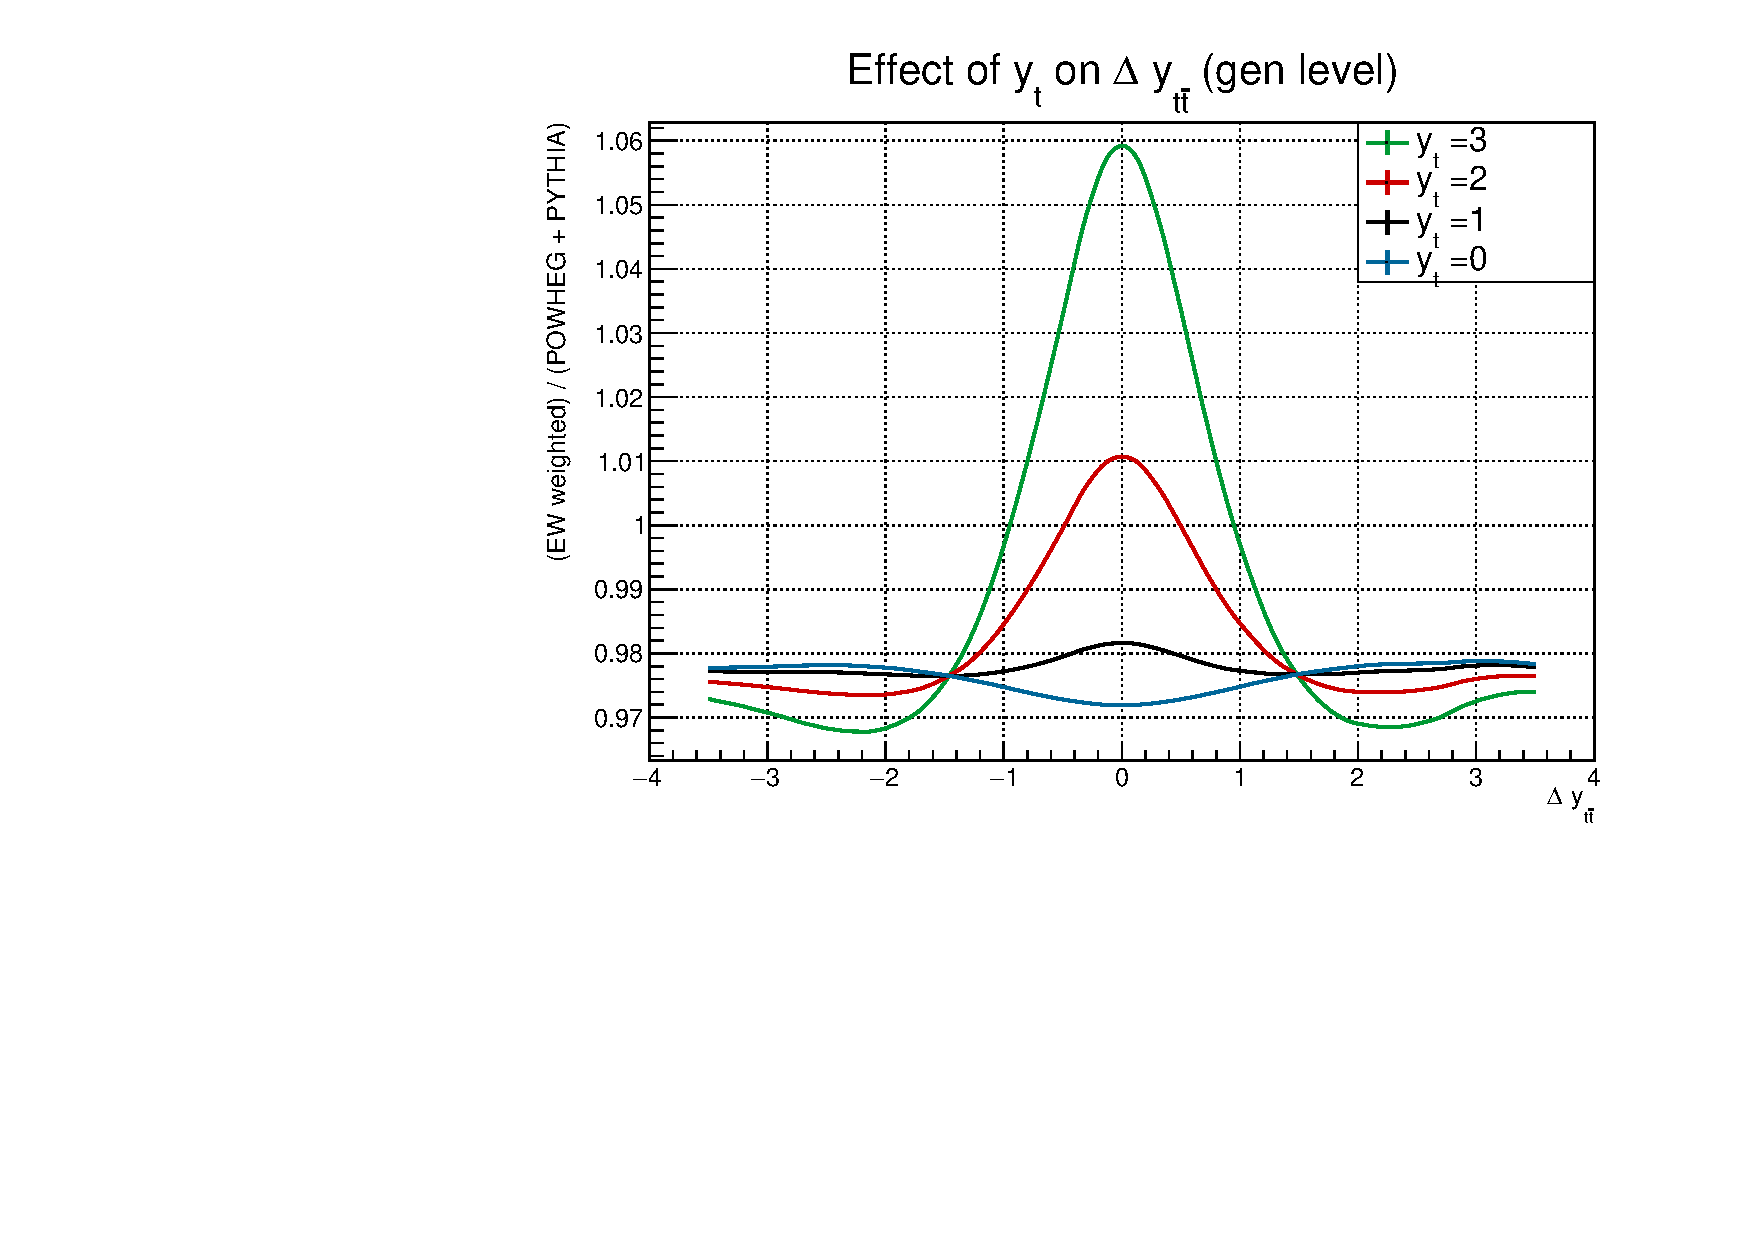
\includegraphics[width=.48\linewidth]{figs/ratDyttgen.pdf}
    \caption{Effect of the EW corrections on \ttbar differential kinematic distributions for different values of $\yt$, after reweighting of gen-level events from Powheg+Pythia8}
    \label{fig:hatratgen}
\end{figure}




Thus, the effect of EW corrections can be considered without generating new MC samples. This is achieved by applying  weight corrections to the current standard \ttbar MC samples used by the CMS TOP group. Contributions to the top quark pair production due to the interference of QCD+EW diagrams, shown in Figure \ref{fig:diagrams},  with the leading order (LO) QCD diagrams are evaluated using HATHOR (v2.1) package~\cite{hathorart}. The ratio of these contributions to the LO QCD production is applied as parton-level weight corrections to events simulated using POWHEG+PYTHIA8, which incorporates fully NLO QCD calculations and parton shower effects \cite{Nason:2004rx,Frixione:2007vw,Alioli:2010xd,Campbell:2014kua,Sjostrand:2006za,Sjostrand:2007gs} \cite{Frederix:2012ps}. In HATHOR, we can control the ratio of the Yukawa coupling used in computing the Electroweak corrections to the standard model value, 
\begin{equation}
\yt = g_\mathrm{t}\mathrm{(HATHOR)}/g_\mathrm{t}\mathrm{(SM).} 
\end{equation}

Weights are calculated for discrete integer values of $\yt=0,1,\ldots,5.$ After event reconstruction, data from the discrete values is interpolated to generate a continuous template as a function of $\yt$. Using this parameterization we are able to perform a maximum likelihood fit and obtain an estimate for $\yt$ based on the kinematic distributions observed in data. 

Our aim is to take this approach, which has been successfully applied to \ttbar decays in the lepton+jets channel \cite{ytpaper}, and apply it to the dilepton channel. While this channel has a smaller branching ratio, it has much lower backgrounds due to the distinguishing presence of two final state leptons. However, it also contains two final state neutrinos, presenting the question of whether it is necessary to perform a full kinematic reconstruction with two missing final state particles. 

In this note, we will discuss first our Data/MC samples (Section \ref{S:data}), followed by our methods for event selection (Section \ref{S:selection}) and reconstruction (Section \ref{S:reco}). We then present an outline of the measurement technique (Section \ref{S:stats}), followed by a detailed consideration of uncertainty sources and their treatment (Section \ref{S:sys}). We conclude with a preliminary sensitivity study done on the Asimov dataset, demonstrating the current expected sensitivity of our measurement (Section \ref{S:fit}).

\clearpage


\section{The CMS detector}
\label{sec:detector}
The central feature of the CMS detector is a superconducting solenoid of 6m internal diameter,
providing a magnetic field of 3.8 T. Within the solenoid volume are a silicon pixel and strip
tracker, a lead tungstate crystal electromagnetic calorimeter (ECAL), and a brass and scintillator
hadron calorimeter (HCAL), each composed of a barrel and two endcap sections. Forward calorimeters
extend the coverage provided by the barrel and endcap detectors. Muons
are measured in gas-ionization detectors embedded in the steel flux-return yoke outside the
solenoid. 

The particle-flow (PF) algorithm~\cite{CMS-PRF-14-001} aims to reconstruct and identify each individual particle in an event, with an optimized combination of information from the various elements of the CMS detector. The energy of photons is obtained from the ECAL measurement. The energy of electrons is determined from a combination of the electron momentum at the primary interaction vertex as determined by the tracker, the energy of the corresponding ECAL cluster, and the energy sum of all bremsstrahlung photons spatially compatible with originating from the electron track. The energy of muons is obtained from the curvature of the corresponding track. The energy of charged hadrons is determined from a combination of their momentum measured in the tracker and the matching ECAL and HCAL energy deposits, corrected for zero-suppression effects and for the response function of the calorimeters to hadronic showers. Finally, the energy of neutral hadrons is obtained from the corresponding corrected ECAL and HCAL energies.A more detailed description of the CMS detector, together with a definition of the
coordinate system and relevant kinematical variables, can be found in Ref. ~\cite{Chatrchyan:2008zzk}.

\section{Data and Monte Carlo (MC) Samples}



We utilize the full CMS Run 2 dataset. Events are selected from the SingleMuon and SingleElectron/EGamma data streams. As the \ttbar dilepton channel  overall has very low background level, we rely on Monte Carlo simulation to estimate their rates and kinematic distributions. In particular, we  account for dilepton production due to Drell-Yan type processes and single top production. Backgrounds from QCD multijet production were found to be negligible and are not included. Among vector+jets backgrounds, W decay samples were also investigated and found to have negligible contributions. 

Around 1\% of events identified as \ttbar dilepton are in fact misidentified \ttbar lepton+jets events.  EW corrections are applied to all \ttbar events,  even  misidentified ones. This approach also allows us to apply systematic uncertainty variations to the ttbar sample uniformly.

The full list of Monte Carlo samples used by this analysis is shown in Tables \ref{tab:2016MC}--\ref{tab:2018MC}.  Expected signal and background counts, after event selection, are discussed in Section \ref{SS:bg}.

\label{S:data}

\clearpage
\section{Event Selection}
\label{S:selection}

\subsection{Trigger}
\label{SS:trigger}
 Events are selected from the SingleMuon and SingleElectron/EGamma data streams if they pass single lepton triggers. based on availability of different $p_T$ triggers, in the muon channel we use a $p_T$ threshold of 24/27/24 GeV  in 2016/2017/2018 datasets respectively, and for electrons a $p_T$ threshold of 27/27/32 in 2016/2017/2018. To avoid a double counting of events, all events selected by the chosen muon triggers are rejected in the SingleElectron/EGamma data stream. 


\subsection{Leptons}
Due to the use of single-lepton triggers, we require that at least one lepton pass a leading $p_T$ selection above the online trigger threshold. We then require that an additional lepton of opposite sign passes a less stringent sub-leading $p_T$ selection. We reject events with more than 2 leptons passing the sub-leading $p_T$ selection.

\subsection*{Muons}
The pseudo-rapidity is restricted to the silicon tracker coverage of $\abs{\eta} < 2.4$. A cut-based selection is applied and isolation required. Muons are categorized as isolated if the particle-flow (PF) isolation $I_\mathrm{PF}/p_T(\mu) < 0.15$, where $I_\mathrm{PF} = I_\mathrm{CH} + \max(0, I_\mathrm{N} + I_\mathrm{PH} - 0.5 I_\mathrm{CH,pu})$ and $I_\mathrm{X}$ if the $p_T$-sum of charged (CH), neutral (N), and photon-like (PH) particle-flow candidates within $\Delta R = 0.4$ around the muon. The last term $I_\mathrm{CH,pu}$, which is the sum of charged particles not originating from the main primary vertex, is designed to compensate for contributions from pileup. 

The leading muon $p_T$ is requires to be greater than $30$\,GeV. This ensures that the offline selection is well above the trigger threshold of 27\,GeV. For the sub-leading muons, we require  $p_T>15$\,GeV.

Efficiencies of reconstruction, identification and the trigger have been studied and scale factors are applied to the simulation based on a tag and probe method applied to leptons originating from $Z$ boson decay. The corresponding systematic uncertainty is  described in Section \ref{S:sys}.

\subsection*{Electrons}
 We restrict the pseudo-rapidity to the silicon tracker coverage of $\abs{\eta} < 2.4$. Electrons with an ECal super cluster (SC) in the gap between the barrel and the endcap, $1.442 < \eta(SC) < 1.566$, are rejected. A cut-based ID is used, which includes an isolation requirement similar to muons. In addition, a selection on the transverse impact parameter $\abs{d_\mathrm{0}} < 0.05(0.10)$\,cm and the longitudinal impact parameter $\abs{d_\mathrm{z}} < 0.1(0.2)$\,cm is applied in the barrel(endcap) regions.
 
 In 2016 and 2017 datasets the trigger $p_T$ threshold for isolated electrons is 27\,GeV, although there were periods in 2017, when the trigger based on electrons with  $p_T$ below  32\,GeV was pre-scaled. For both 2016 and 2017 we choose to use an offline selection of  $p_T > 30$\,GeV, and to treat the pre-scales in 2017 as an additional inefficiency. In 2018 the  trigger threshold was raised to 32\,GeV and an offline leading $p_T$ cut of $p_T>34$\,GeV is used. In all years, the sub-leading electron requirement is only $p_T>15$\,GeV.

 Scale factors are generated, applied, and considered as uncertainty sources following the same methods used for muons.

\subsection{Jets and b-jet identification}
The default jets are clustered from PF objects using the anti-$k_T$ jet algorithm with a distance parameter of 0.4. Charged particles originating from a pileup interaction vertex are excluded. 

The DeepCSV b-tagging algorithm  is used for the identification of b-jets \cite{deepCSVref}. We require at least two b-jets to pass the loose working point selection criterion. Scale factors derived on data are used to correct the tagging and mistagging efficiencies. Uncertainty on these efficiencies is discussed in Section \ref{S:sys}.

 In events with more than two b-tagged jets, the jets are sorted by the CSV discriminant, with the two leading-CSV jets assumed to be the most likely candidates for b-jets originating from a top decay. After sorting, if the third jet has a similar CSV value to the second (difference $<0.25$), the event is discarded as it is considered unclear which b-jets to use. This is a rare enough occurrence that it is not clear whether it would be worthwhile to invest more effort in selecting 2 b-jets from 3 or more candidates. 
 
 We find that in \ttbar events, the two b-jets are among the candidates passing the loose DeepCSV working point in roughly 93\% of events. In cases where a collection of 3 or more candidates does include the correct b-jets, our simple CSV-sort and cut yields a \ttbar sample where the two b-jets are correctly chosen in 89\% of events.
   


\subsection*{Drell-Yan background removal}

In order to remove Drell-Yan background resulting from $Z\ \gamma \rightarrow e^+e^- $ or $Z \ \gamma \rightarrow \mu^+\mu^-$, we apply some additional selection criteria in the $ee$ and $\mu\mu$ channels. We require that the invariant mass of the two leptons, $M_{l\bar{l}}$ is not within $10$ \unit{GeV} of the $Z$-boson mass, 91.2 \unit{GeV}. Additionally, we require $M_{l\bar{l}}$  above 50\,GeV and in order to match the Monte Carlo sample used for Drell-Yan background modelling. 

Additionally, we apply selection based on a missing transverse momentum, MET, of $p_{T}\mathrm{,miss}>30$ \unit{GeV}. These selection criteria remove the majority of Drell-Yan background. 

\subsection{Additional Corrections}
\par \noindent
\textbf{Pileup }

Pileup reweighting is applied to adjust the number of interactions generated in the Monte Carlo to match the data. A corresponding uncertainty is discussed in Section \ref{S:sys}.

\par \noindent
\textbf{ECAL L1 prefire }

A re-weighting is performed to address the problem with pre-firing of the EG L1 trigger in the ECAL endcap, which was present in 2016-2017 data taking periods. A corresponding uncertainty is discussed in Section \ref{S:sys}.

\subsection{Event yields \& background estimation}
\label{SS:bg}

The breakdown of expected signal and background counts is shown by year in Table \ref{tab:eventcounts}. The vector+jets background, which originates almost entirely from Drell-Yan same-flavor lepton production, is estimated to be reduced to around 2\%. Decays from single top production account for roughly another 2\% of the estimated sample composition. Despite some differences in kinematic distributions in the $e\mu$ channel and the same-flavor channels, where Drell-Yan suppression selection is applied, there was no clear benefit in separating the decay channels by lepton flavor.


\begin{table}[]
\centering

\begin{tabular}{ l | c | c }
2016 & yield ($\pm \sigma_\mathrm{stat}$) & \% of total MC \\ \hline
\ttbar\;signal MC & 139617\;$\pm$\;164.7 & 96.6\% \\ 
vector + jets MC & 1947\;$\pm$\;53.7 & 1.3\% \\ 
single top MC & 3013\;$\pm$\;25.3 & 2.1\% \\ 
\hline total MC  & 144578\;$\pm$\;175.0 & 100\% \\ 
\hline data  & 144188 & 99.7\% \\ 
\end{tabular}

\vskip.6cm
\begin{tabular}{ l | c | c }
2017 & yield ($\pm \sigma_\mathrm{stat}$) & \% of total MC \\ \hline
\ttbar\;signal MC & 168778\;$\pm$\;94.4 & 95.6\% \\ 
\ttbar\;background MC & 1052\;$\pm$\;12.1 & 0.6\% \\ 
vector + jets MC & 3214\;$\pm$\;75.2 & 1.8\% \\ 
single top MC & 3513\;$\pm$\;24.0 & 2.0\% \\ 
\hline total MC  & 176558\;$\pm$\;123.7 & 100\% \\ 
\hline data  & 177182 & 100.4\% \\ 
\end{tabular}
\vskip.6cm
\begin{tabular}{ l | c | c }
2018 & yield ($\pm \sigma_\mathrm{stat}$) & \% of total MC \\ \hline
\ttbar\;signal MC & 242689\;$\pm$\;140.0 & 95.7\% \\ 
\ttbar\;background MC & 1416\;$\pm$\;17.4 & 0.6\% \\ 
vector + jets MC & 4624\;$\pm$\;128.1 & 1.8\% \\ 
single top MC & 4907\;$\pm$\;26.9 & 1.9\% \\ 
\hline total MC  & 253636\;$\pm$\;192.4 & 100\% \\ 
\hline data  & 261507 & 103.1\% \\ 
\end{tabular}





    \caption{MC and data event yields for all 3 years. Statistical uncertainty on simulated event counts is given. For estimates of systematic uncertainty, see Figures \ref{fig:dmcpre_16}--\ref{fig:dmcpost_18}.}
    \label{tab:eventcounts}
\end{table}



\clearpage
\section{Event Reconstruction}
\label{S:reco}

\begin{figure}
    \centering
    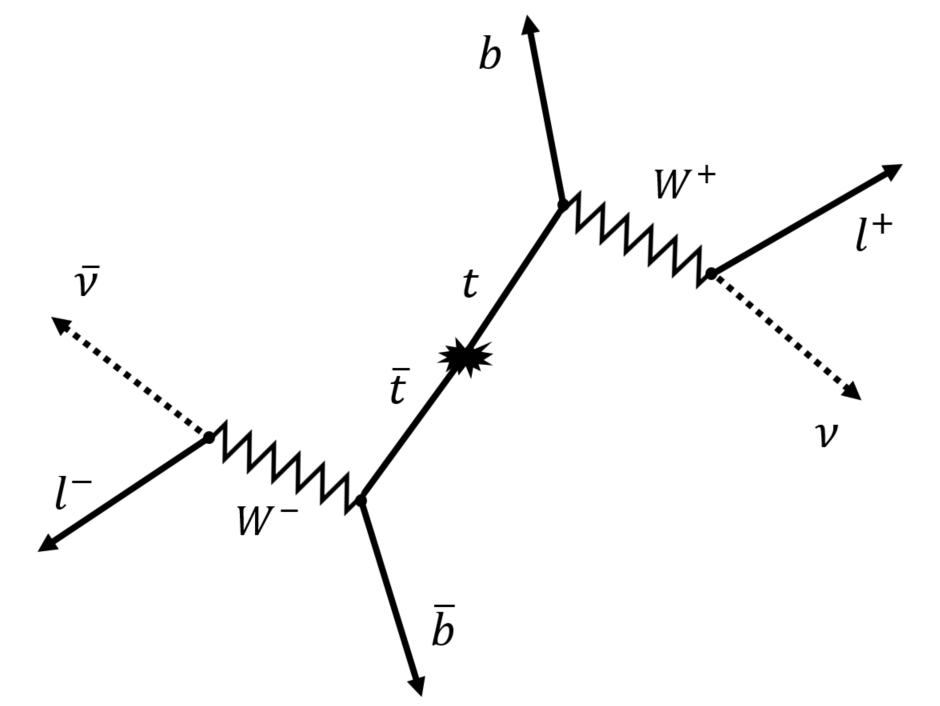
\includegraphics[width=.5\linewidth]{figs/ttbar3.png}
    \caption{Diagram of a \ttbar decay in the dilepton channel. The process can be induced by quark or gluon processes at the LHC.}
    \label{fig:ttdia}
\end{figure}

EW corrections are evaluated as a function of $M_{\ttbar}$ and $|\Delta y|_\ttbar $. To evaluate these quantities it is necessary to reconstruct the full \ttbar kinematics.
%While one might first attempt to reconstruct the full \ttbar kinematics to recover these quantities, it is natural to consider other related kinematic variables as well. 
Figure \ref{fig:ttdia} shows a diagram of \ttbar decay in the dilepton channel. Two neutrinos are present in the final state. While it is possible to completely reconstruct the neutrinos momenta under some assumptions, such reconstruction is highly sensitive to the poorly measured MET. 
%In addition, it is also affected by uncertainty on the jet energy, and comes with a separate systematic uncertainty implemented at the recommendation of the JETMET POG \cite{metunc}.  
We found that a more sensitive measurement results from discarding the neutrino kinematics entirely, using only the kinematics of the better-reconstructed b-jets and leptons. 

We introduce the proxy variables
\begin{eqnarray}
    \Mbl &=& M(b+\bar{b}+l+\bar{l}), \\
    \absDybl &=& |y(b+\bar{l}) - y(\bar{b}+l)|,
\end{eqnarray}
which were found to have good sensitivity to EW corrections while being less vulnerable to resolution effects and systematic uncertainties.

\subsection{b-jet pairing}
\label{SS:bjpair}

After object selection, a two-fold ambiguity remains in pairing the b-jets with the leptons that originates from the same top quark (Figure \ref{fig:ttdia}), i.e. $b\leftrightarrow \bar{l}$, $\bar{b}\leftrightarrow l$. The kinematic variable $\Mbl$, unlike $M_\ttbar$, is independent of this pairing. However, \absDybl\, which provides an increase in sensitivity, is. 
%This is because a coarse binning in $|\Delta y|_{bl}$ helps to distinguish the shape of the signal from shapes produced by systematic uncertainty templates. 
%However, we also benefit from the fact that $\Mbl$, unlike $M_\ttbar$, is independent of this pairing. 

In order to make this pairing, we utilize the information from the kinematic constraints governing the neutrino momenta, but do not perform a full reconstruction.
If one assumes the top quarks and $W$ bosons to be on-shell, the neutrinos momenta are constrained by a set of quadratic equations arising from the conservation of 4-momentum at each vertex. We refer to these kinematic equations, collectively, as the mass constraint. The mass constraint results  in a continuum of possible solutions for neutrino momenta, which geometrically can be presented as  an intersection of ellipsoids in 3D momentum-space (see \cite{burt} for details). For certain values of input momenta of $b$-jets and leptons, these ellipsoids do not intersect at all, and thus the mass constraint cannot be satisfied.

If the mass constraint is satisfied, one can also apply the MET constraint, equating the total missing $p_T$ in the event to the sum of the $p_T$ of the two neutrinos. This constraint reduces the set of possible solutions to a discrete set of 2-4. Just like in the case of the mass constraint, there some values of the input parameters, for which the MET constraint cannot be satisfied. 

%In practice, one can also find an approximate solution as long as the mass constraint can be satisfied \cite{burt}.
This information is useful in picking the correct b-jet pairing (see Figure \ref{fig:bars}). Pairings with no solution to the mass constraint are generally incorrect. When the mass constraint can be satisfied, pairings with a solution to the MET constraint are more likely to be correct. This information is used as part of the pairing procedure.

The full procedure for b-jet pairing is as follows:
\begin{enumerate}

    \item The mass constraint is checked for both possible pairings. If only one pairing is found to satisfy the mass constraint, that pairing is used. If both pairings fail to satisfy the mass constraint, the event is discarded. If both pairings satisfy the mass constraint, we check the MET constraint.
    \item If only one pairing allows for the MET constraint while the other does not, the pairing yielding an exact solution to the MET constraint is used.
    \item If the neutrino kinematics do not suggest a clear pairing, the $b$-jets, $b_1$ and $b_2$, are paired with the leptons ($l$, $\bar{l}$) by minimizing the quantity $$ \Sigma_{1(2)} =\Delta R(b_{1(2)},l)+ \Delta R(b_{2(1)},\bar{l})$$ among the two possible pairings. This method will choose the correct pairing with 74\% accuracy if both $b$-jets have been identified correctly. 

\end{enumerate}
In the end, the correct $b$-jet pairing is selected for approximately 82\% of events, where both $b$-jets are correctly identified.

\begin{figure}
    \centering
    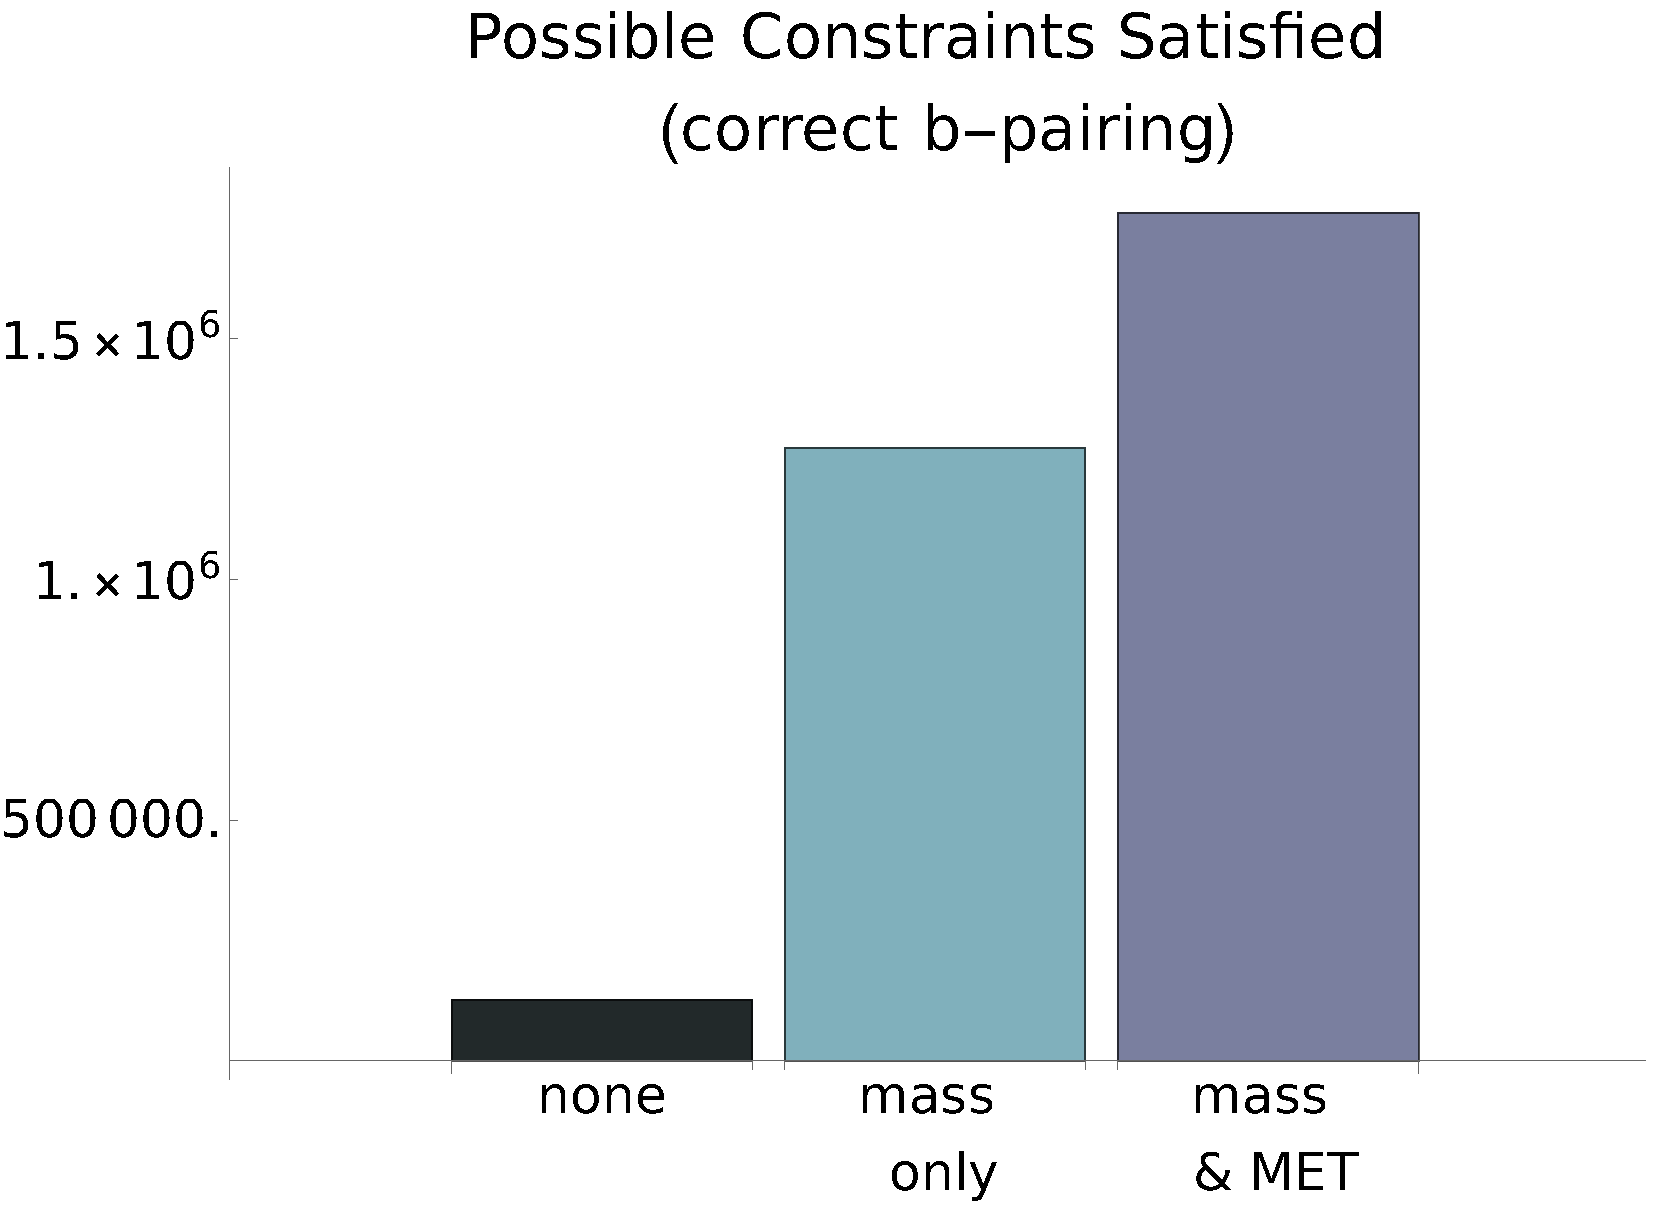
\includegraphics[width=.48\linewidth]{figs/bars_right.pdf} 
    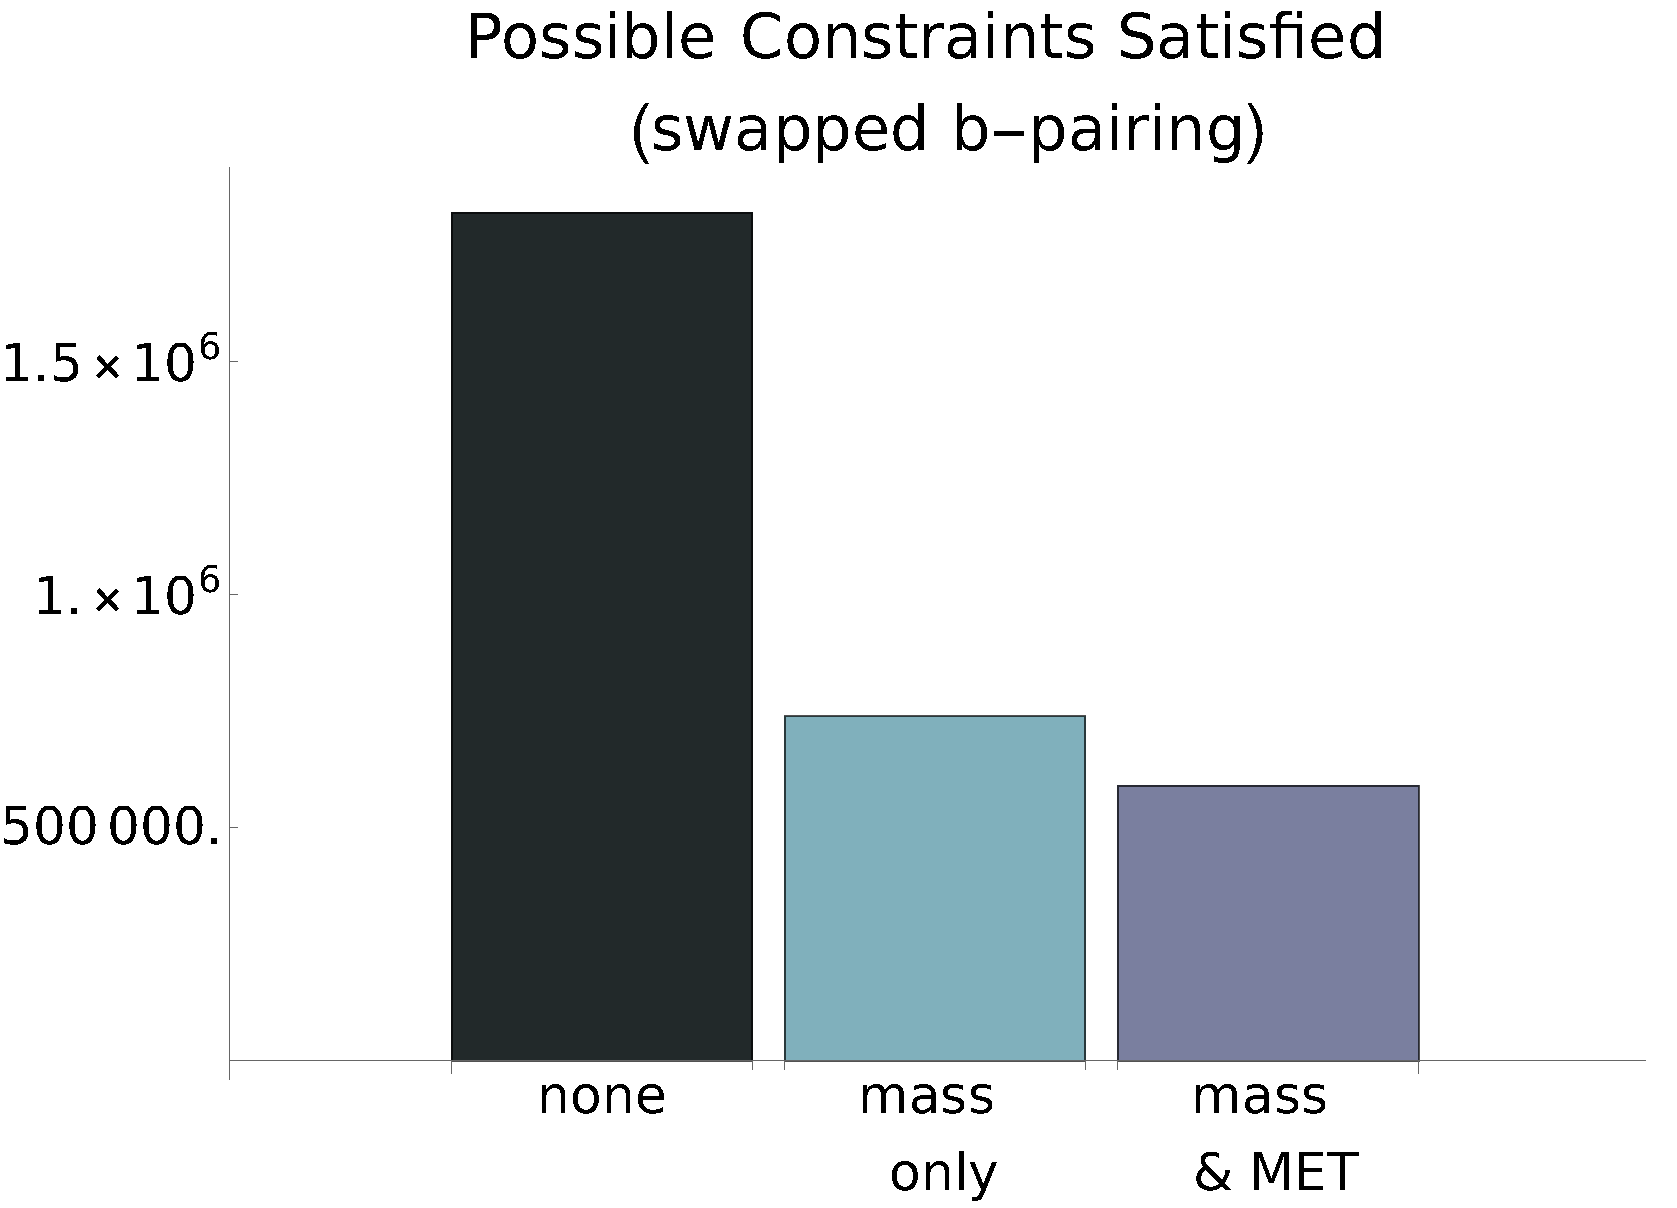
\includegraphics[width=.48\linewidth]{figs/bars_swap.pdf}
    \caption{Distribution over the possible outcomes of the neutrino kinematic constraints assuming correct (left) and swapped (right) b-jet assignment. 
   % These graphs are generated from the same set of events, where both b-jets were correctly identified and reconstructed. We see that, although the kinematic solutions following these constraints are often of poor quality, the possibility to satisfy the kinematic constraints is useful in pairing b-jets with the correct lepton.
    }
    \label{fig:bars}
\end{figure}

\subsection{Sensitivity after reconstruction}
\label{SS:reso}
The sensitivity of our chosen kinematic variables to $\yt$, following reconstruction, is shown in Figure \ref{fig:ratblrec}. The effect of $\yt$ remains substantial enough, and unique enough in shape, that a measurement can be extracted.

\begin{figure}
    \centering
    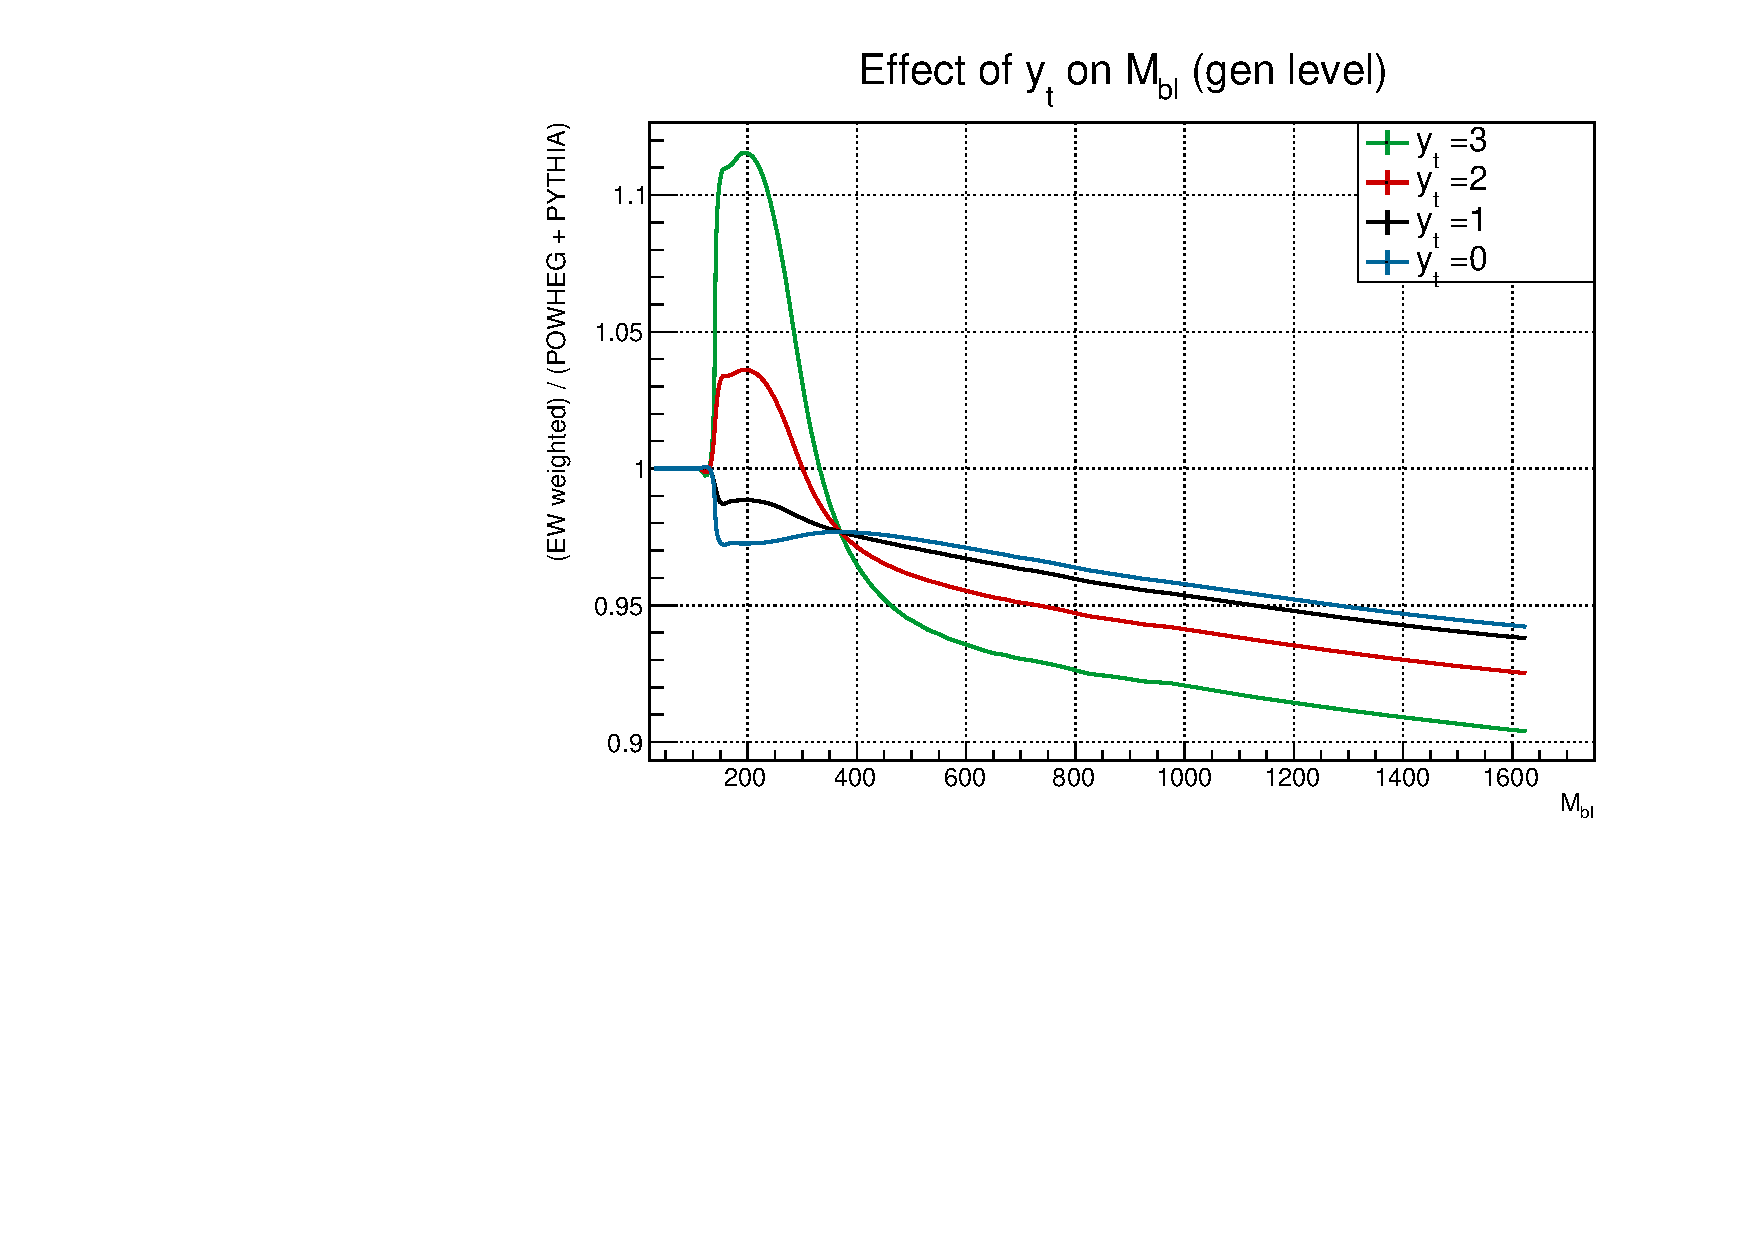
\includegraphics[width=.48\linewidth]{figs/ratMblgen.pdf}
    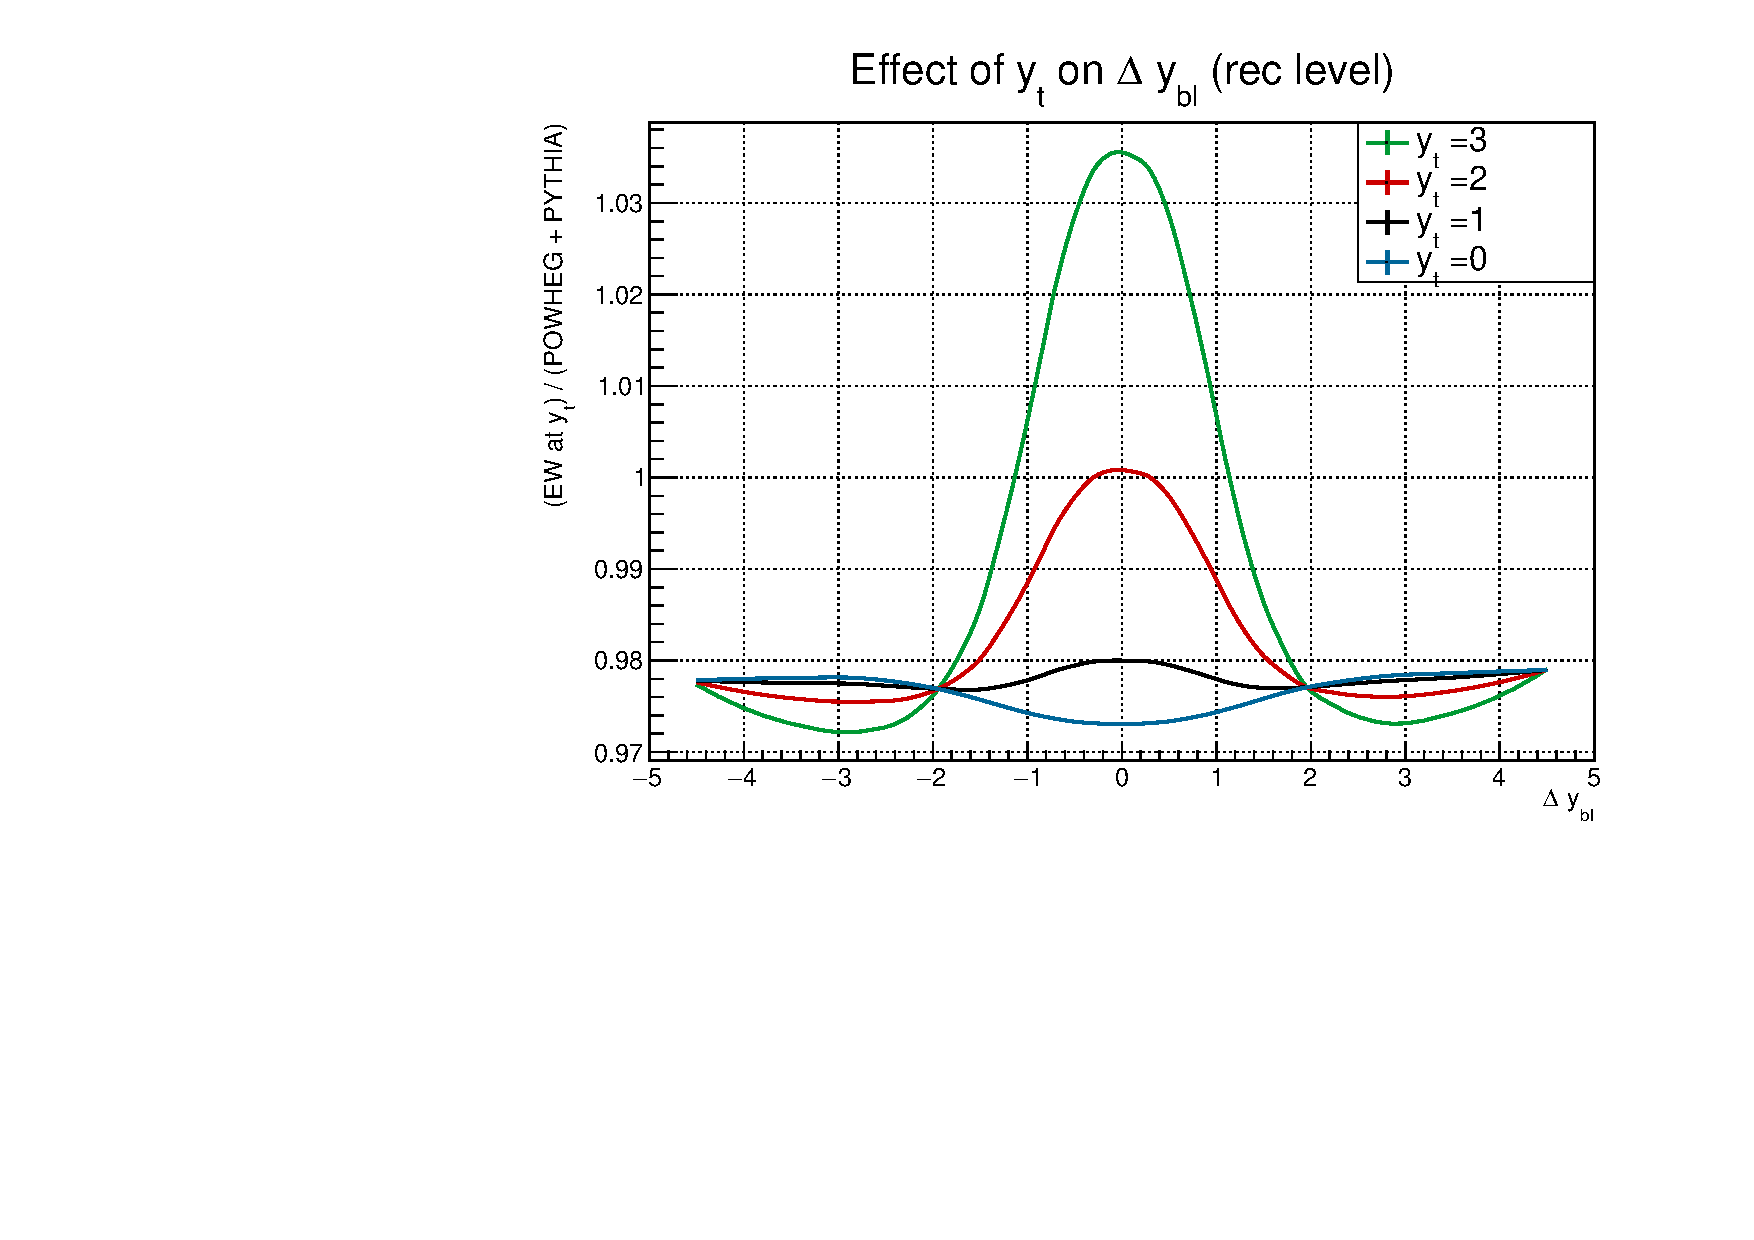
\includegraphics[width=.48\linewidth]{figs/ratDyblgen.pdf}
    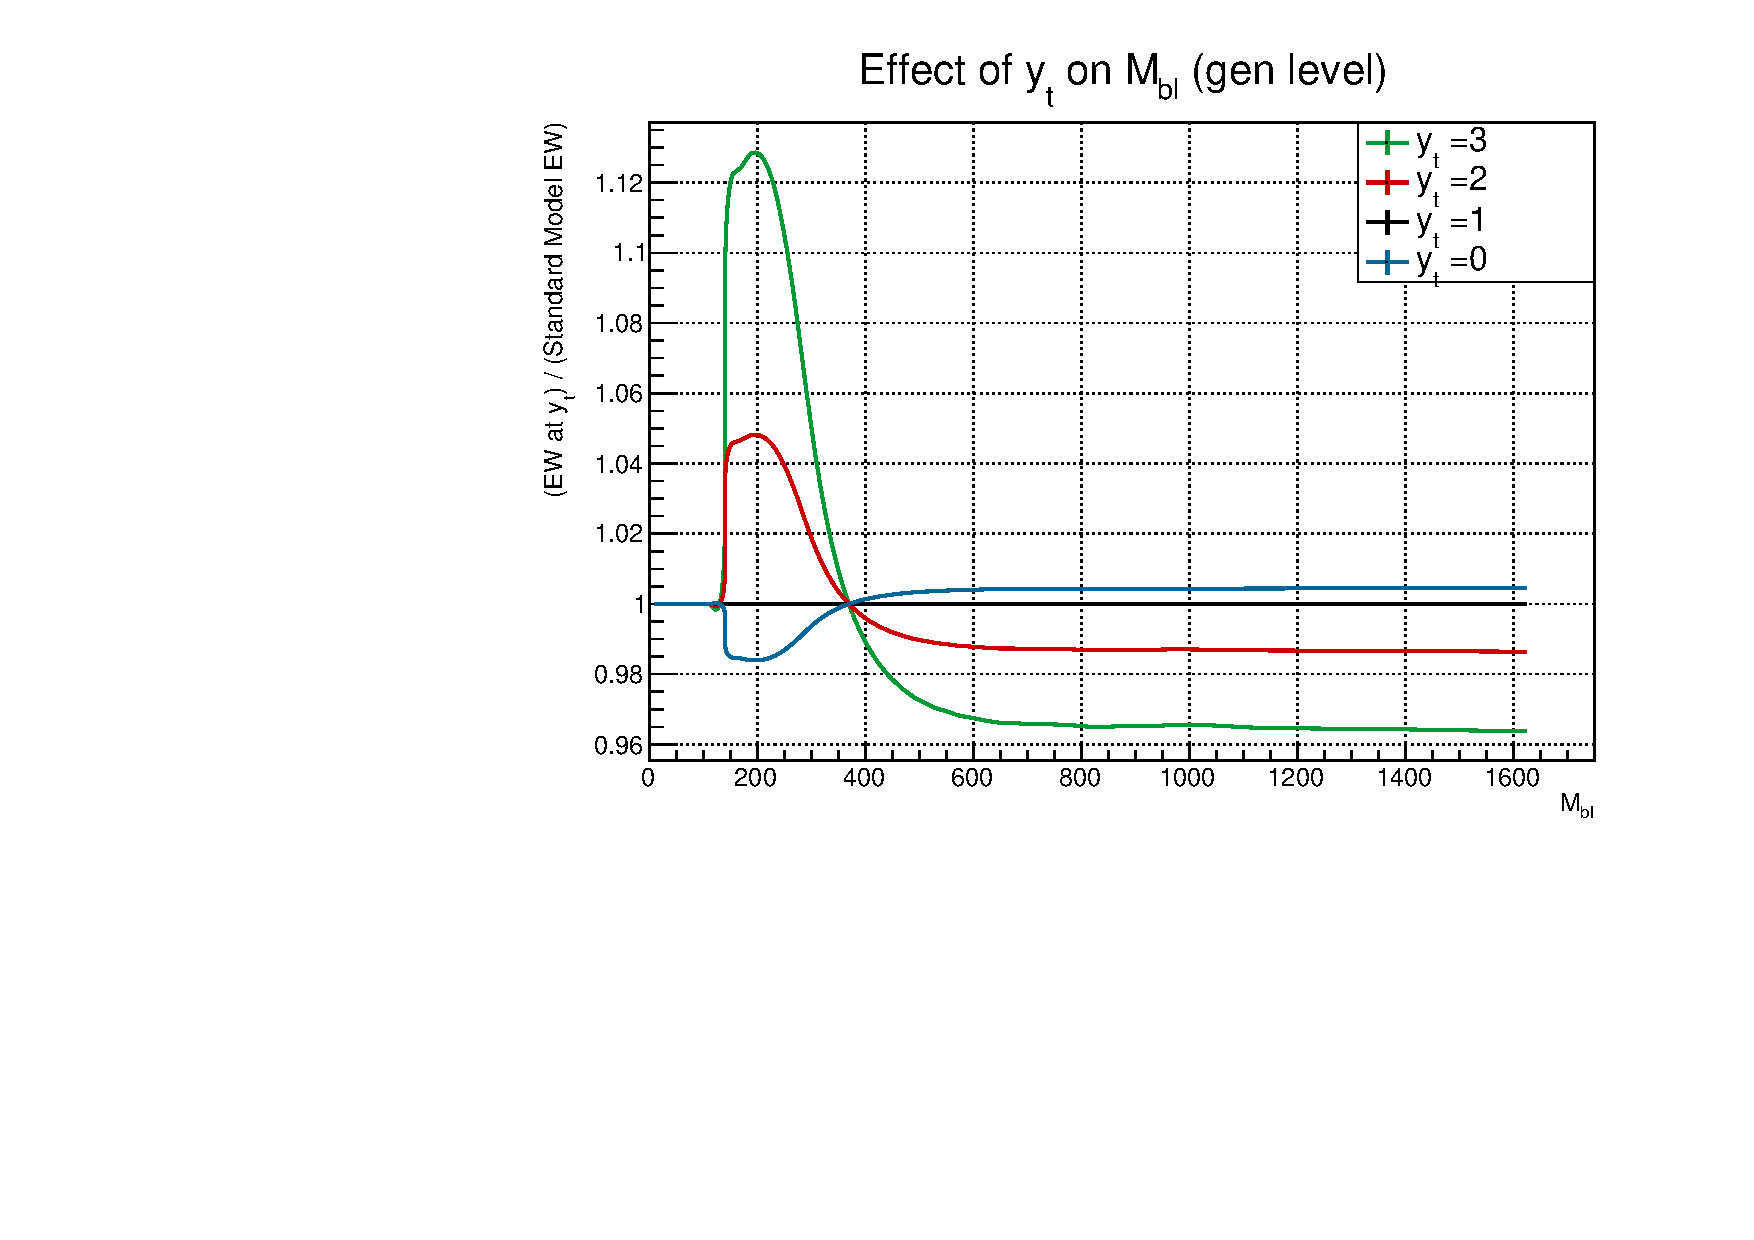
\includegraphics[width=.48\linewidth]{figs/ratMblgen_rel.pdf}
    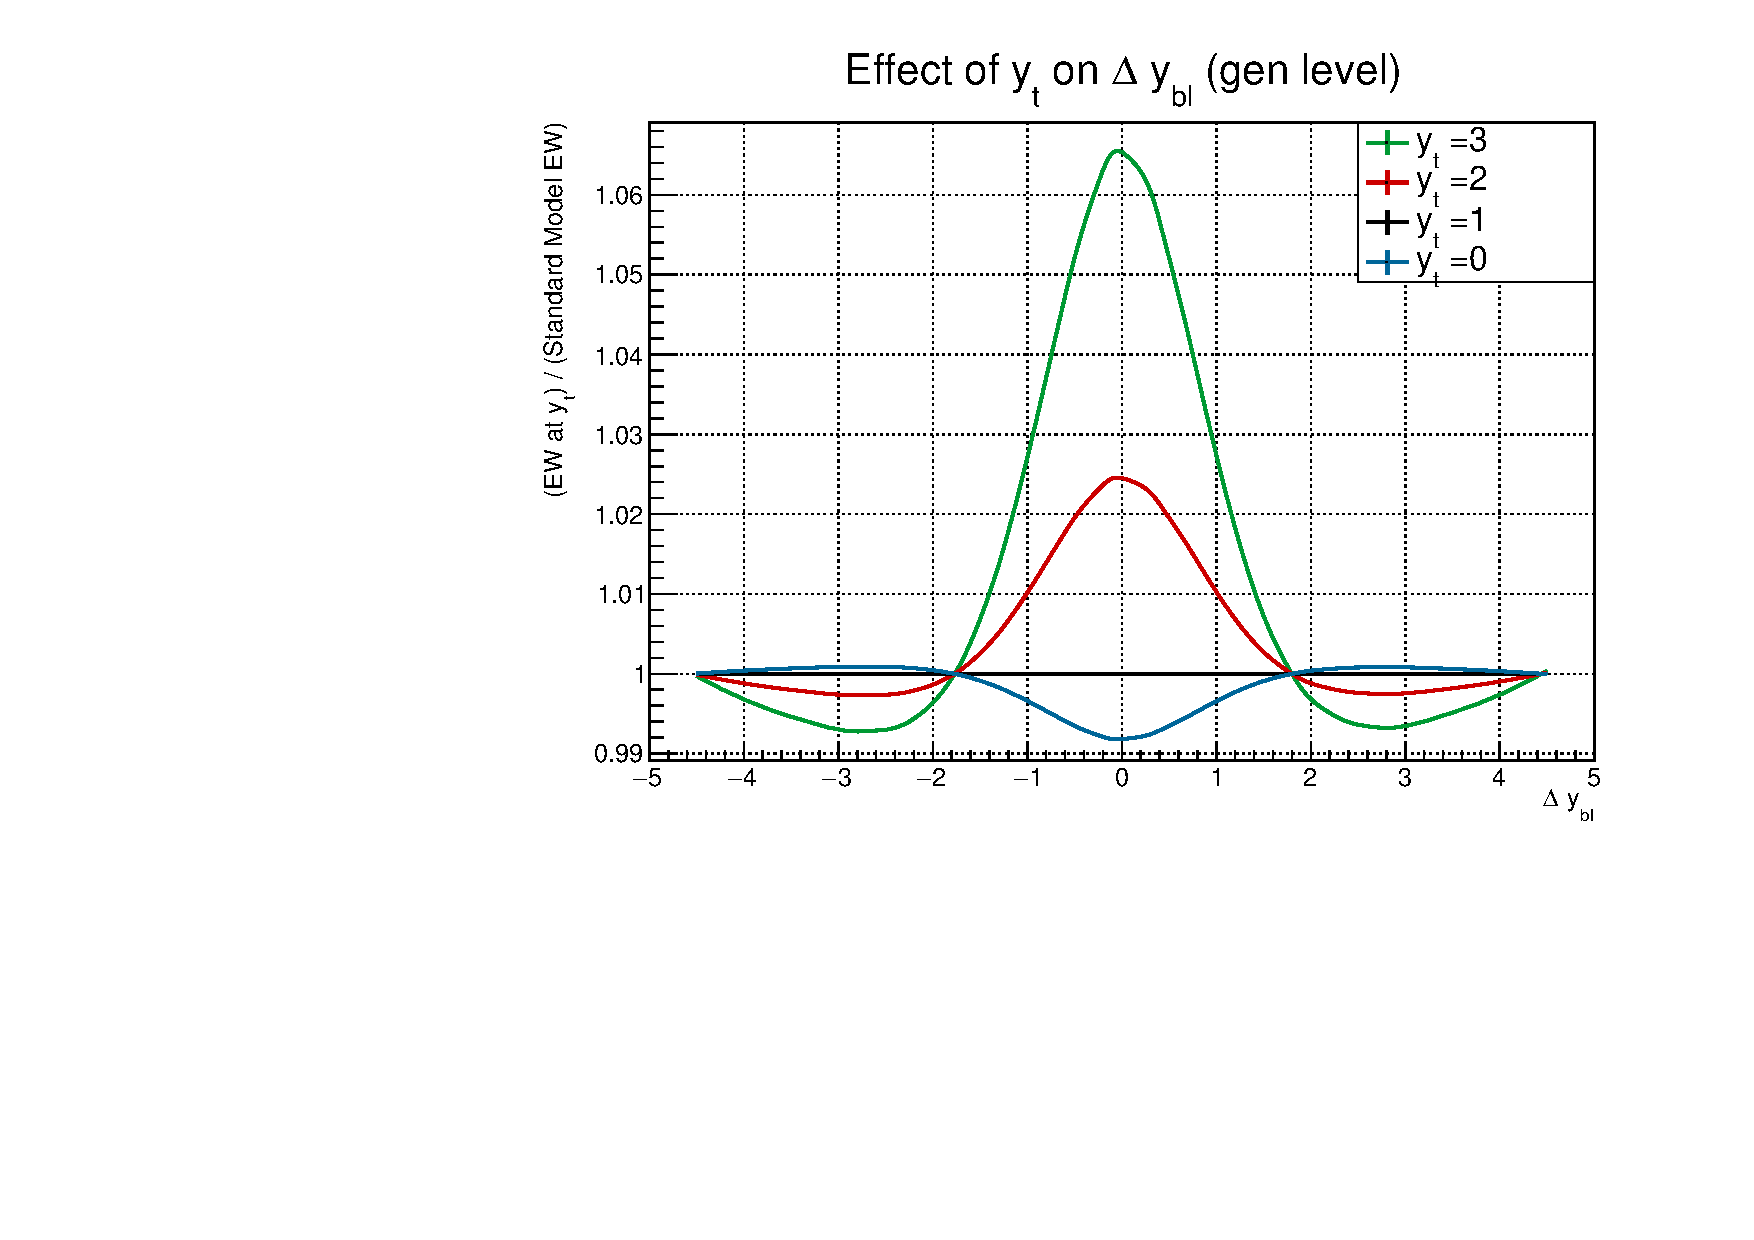
\includegraphics[width=.48\linewidth]{figs/ratDyblgen_rel.pdf}
    \caption{Effect of the EW corrections on kinematic distributions which do not require full kinematic reconstruction of the \ttbar system. The effect is shown both relative to the NLO QCD POWHEG+P8 Monte Carlo Sample (top left \& right), and relative to the Standard Model EW corrections (bottom left \& right). In essence, the top plots show the effect of the EW corrections on the uncorrected sample, while the bottom plots show our sensitivity in distinguishing the effects of different Yukawa coupling values.}
    \label{fig:ratblgen}
\end{figure}

\begin{figure}
    \centering
    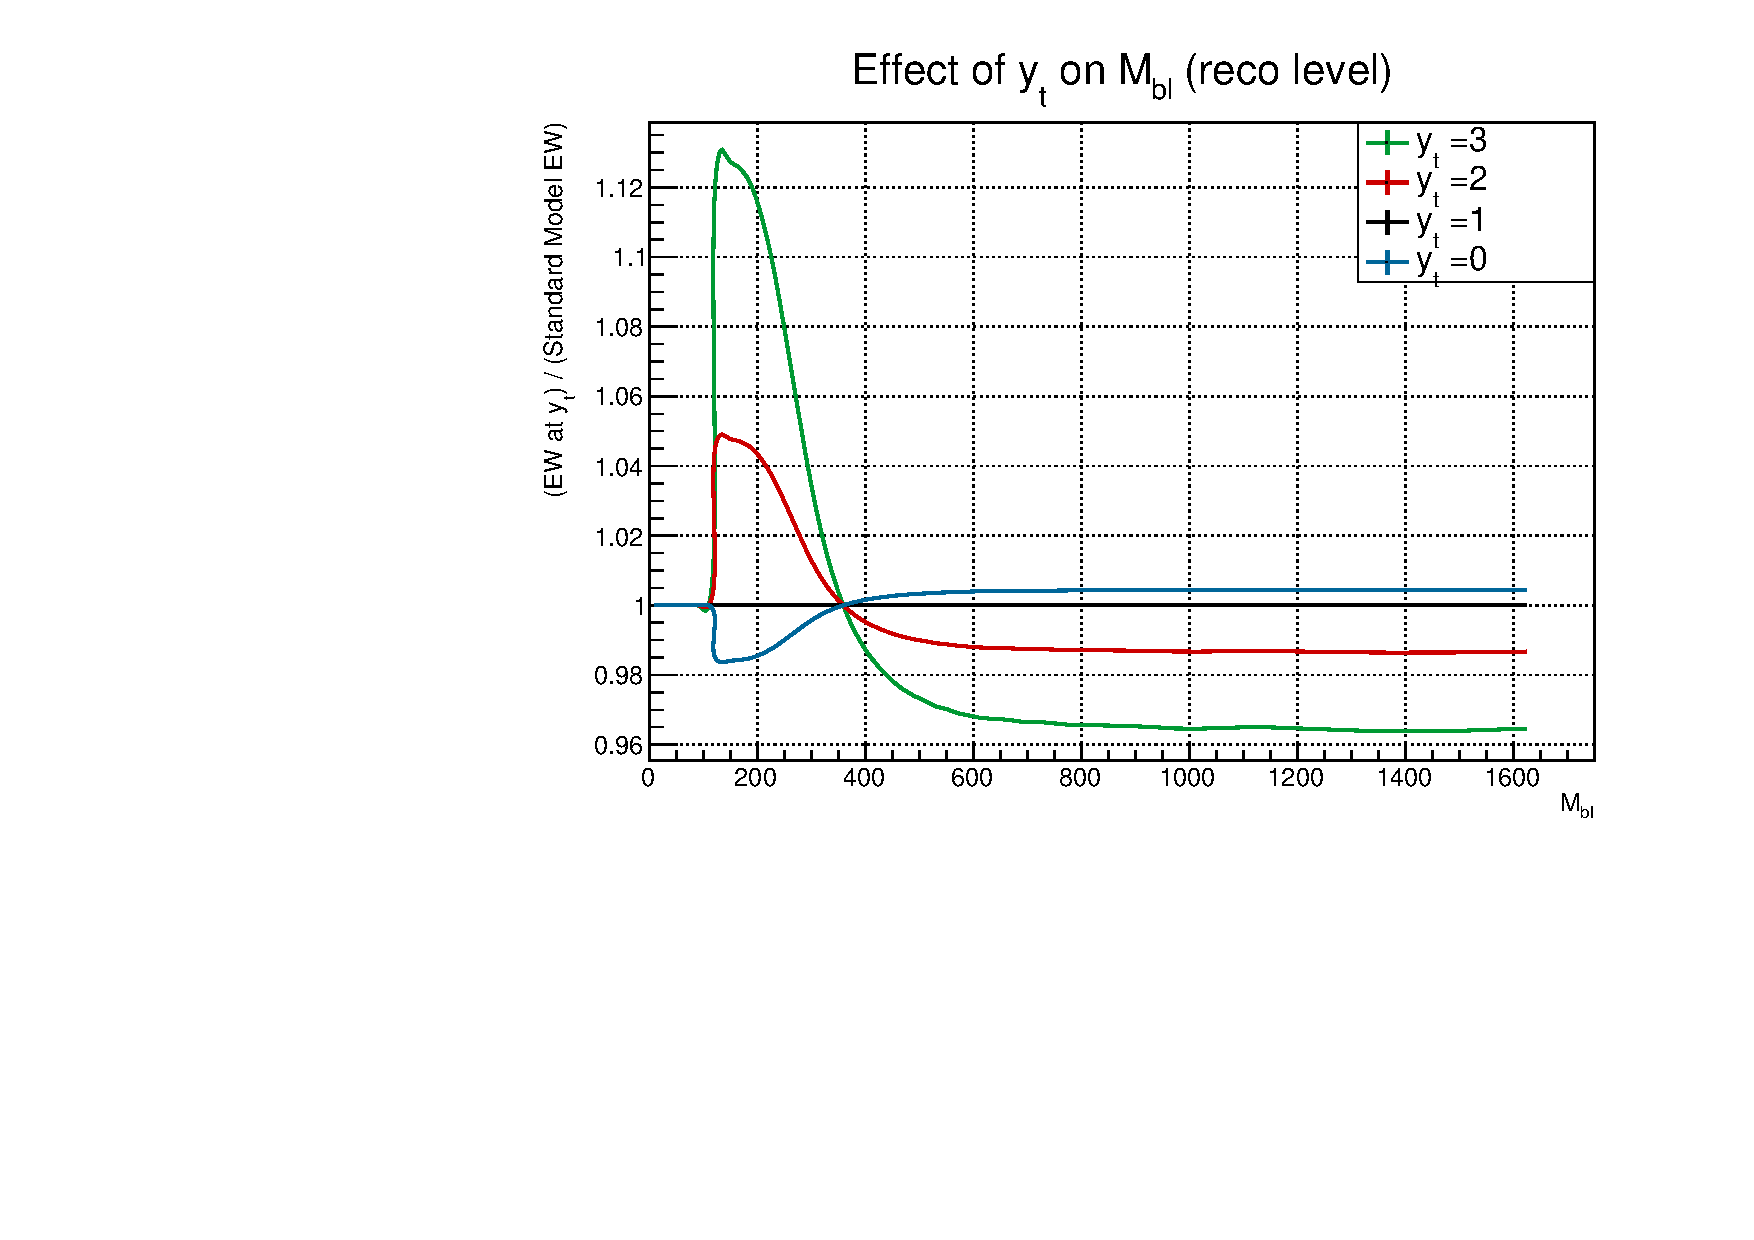
\includegraphics[width=.48\linewidth]{figs/ratMblrec_rel.pdf}
    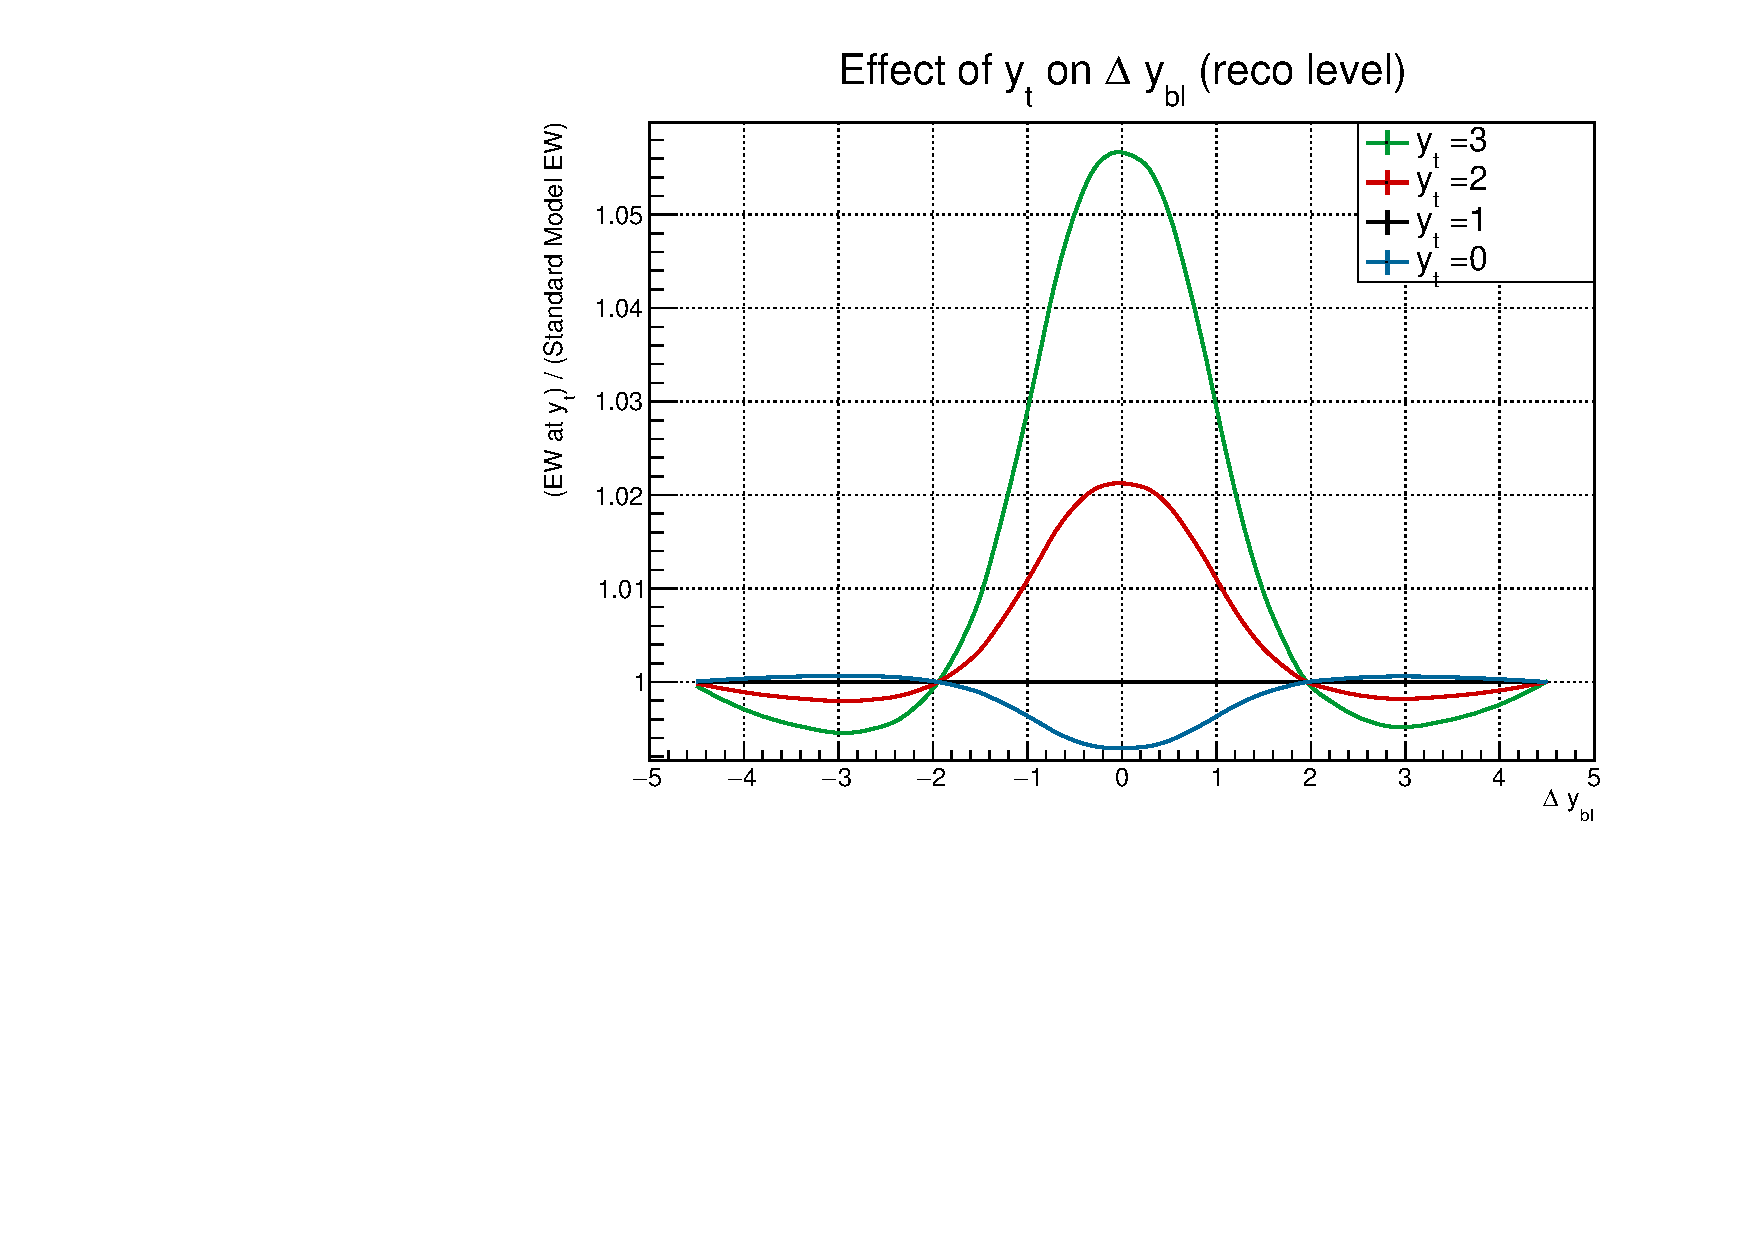
\includegraphics[width=.48\linewidth]{figs/ratDyblrec_rel.pdf}
    \caption{Effect of the EW corrections on \ttbar differential kinematic distributions for different values of $\yt$. We see that the sensitivity to our parameter of interest $\yt$ is not greatly reduced by the reconstruction process, relative to Figure \ref{fig:ratblgen}.}
    \label{fig:ratblrec}
\end{figure}



\subsection{Comparison of distributions from data to \& Monte Carlo prediction}
\label{SS:control}
The comparison between data and Monte Carlo is shown in Figures \ref{fig:dmcpre_16}-\ref{fig:dmcpost_18}. The agreement is generally seen to be well within known uncertainty. We do see some slopes in the ratio of data to MC prediction in the distributions of lepton and $b$-jet $p_T$, to varying extent for each year. These are most likely related to a well know disagreement in top quark $p_T$ distribution. 

It is worth noting that the uncertainty displayed in Figures \ref{fig:dmcpre_16}-\ref{fig:dmcpost_18} can be a bit misleading. Firstly, our parameter of interest is sensitive mainly to shape uncertainties and not to normalization uncertainties. We also include here the uncertainty of the scale variations, which effect the normalization by $\approx 10\%$. However, the $\ttbar$ sample is normalized to the NNLO cross section value, which should better constrain the total cross section normalization, if not the shape. This is accounted for later in the measurement itself, but not reflected in the control plots. 


\begin{figure}[h]
    \centering
    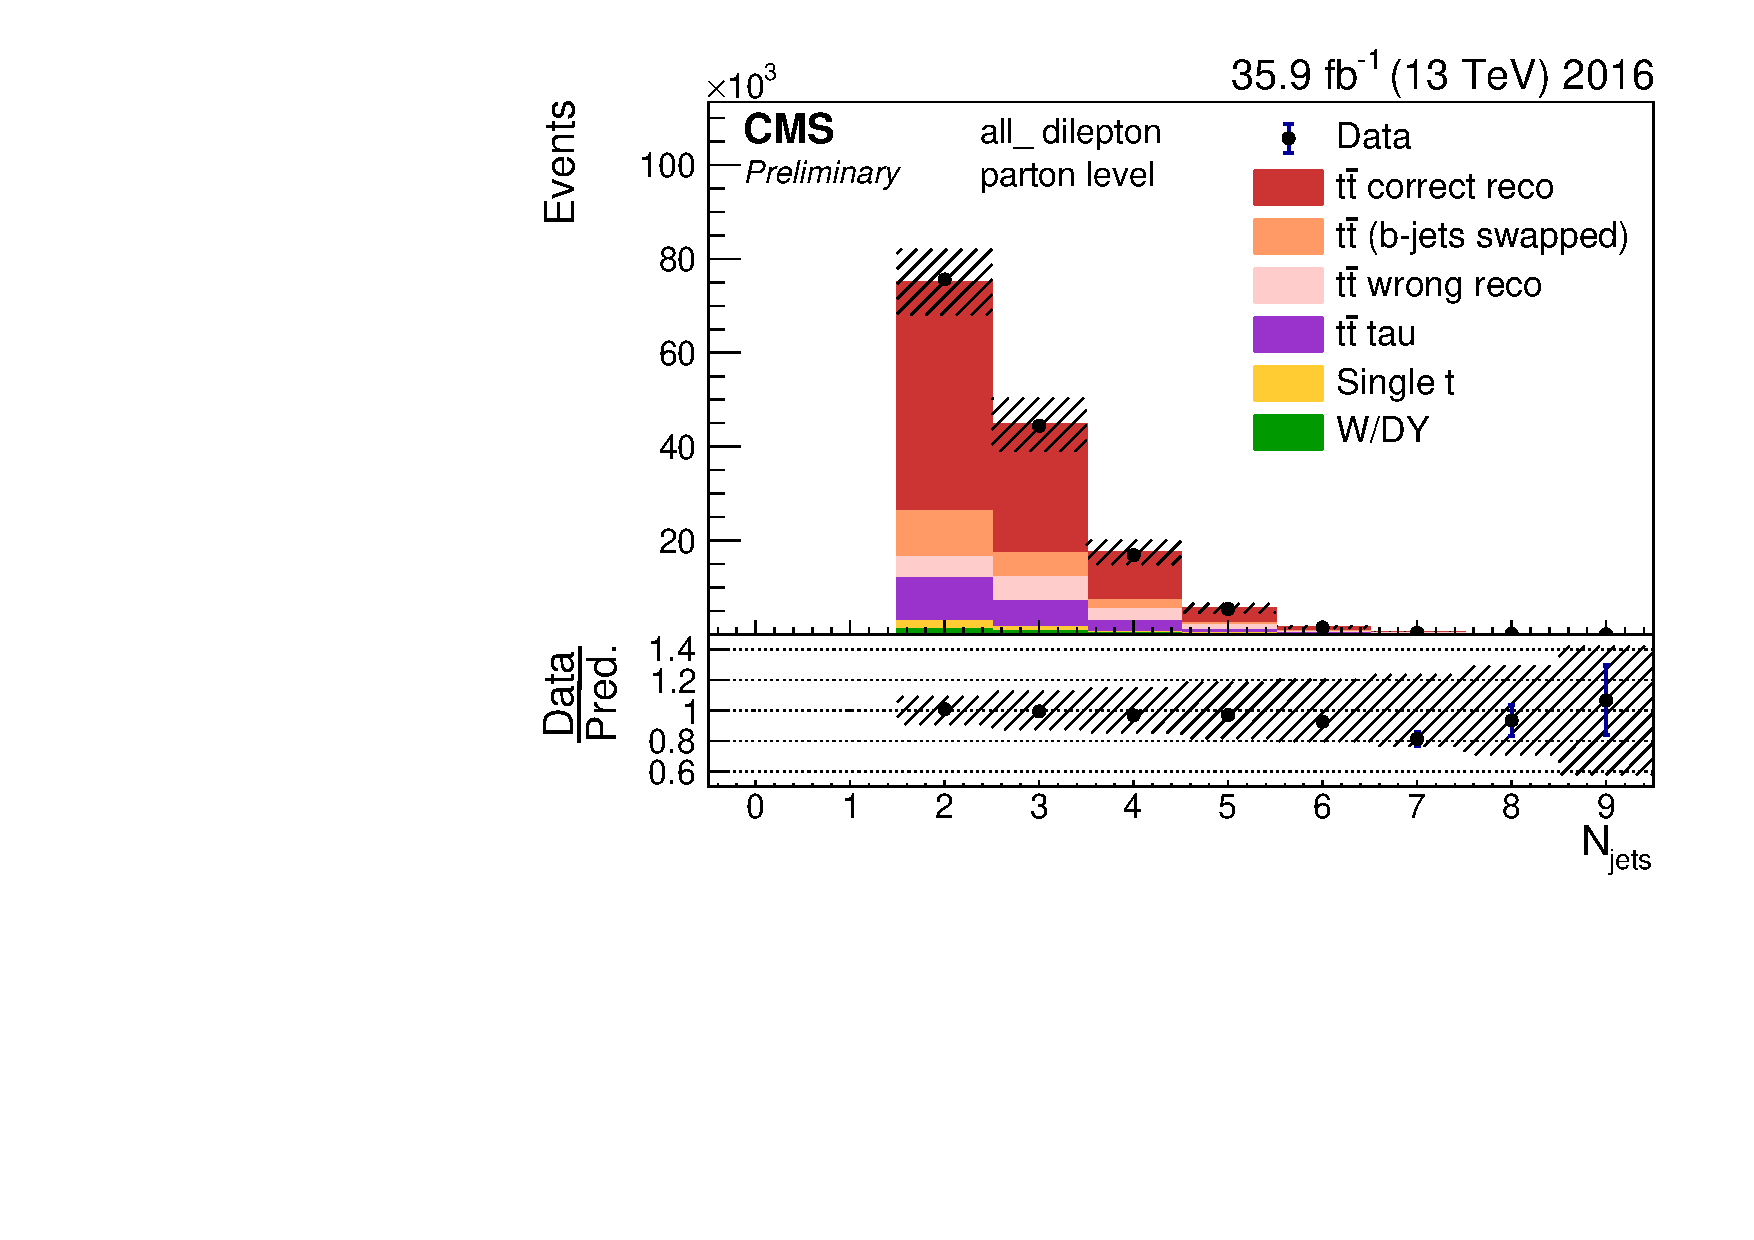
\includegraphics[width=.44\linewidth]{control/16_all_Njets.pdf}
    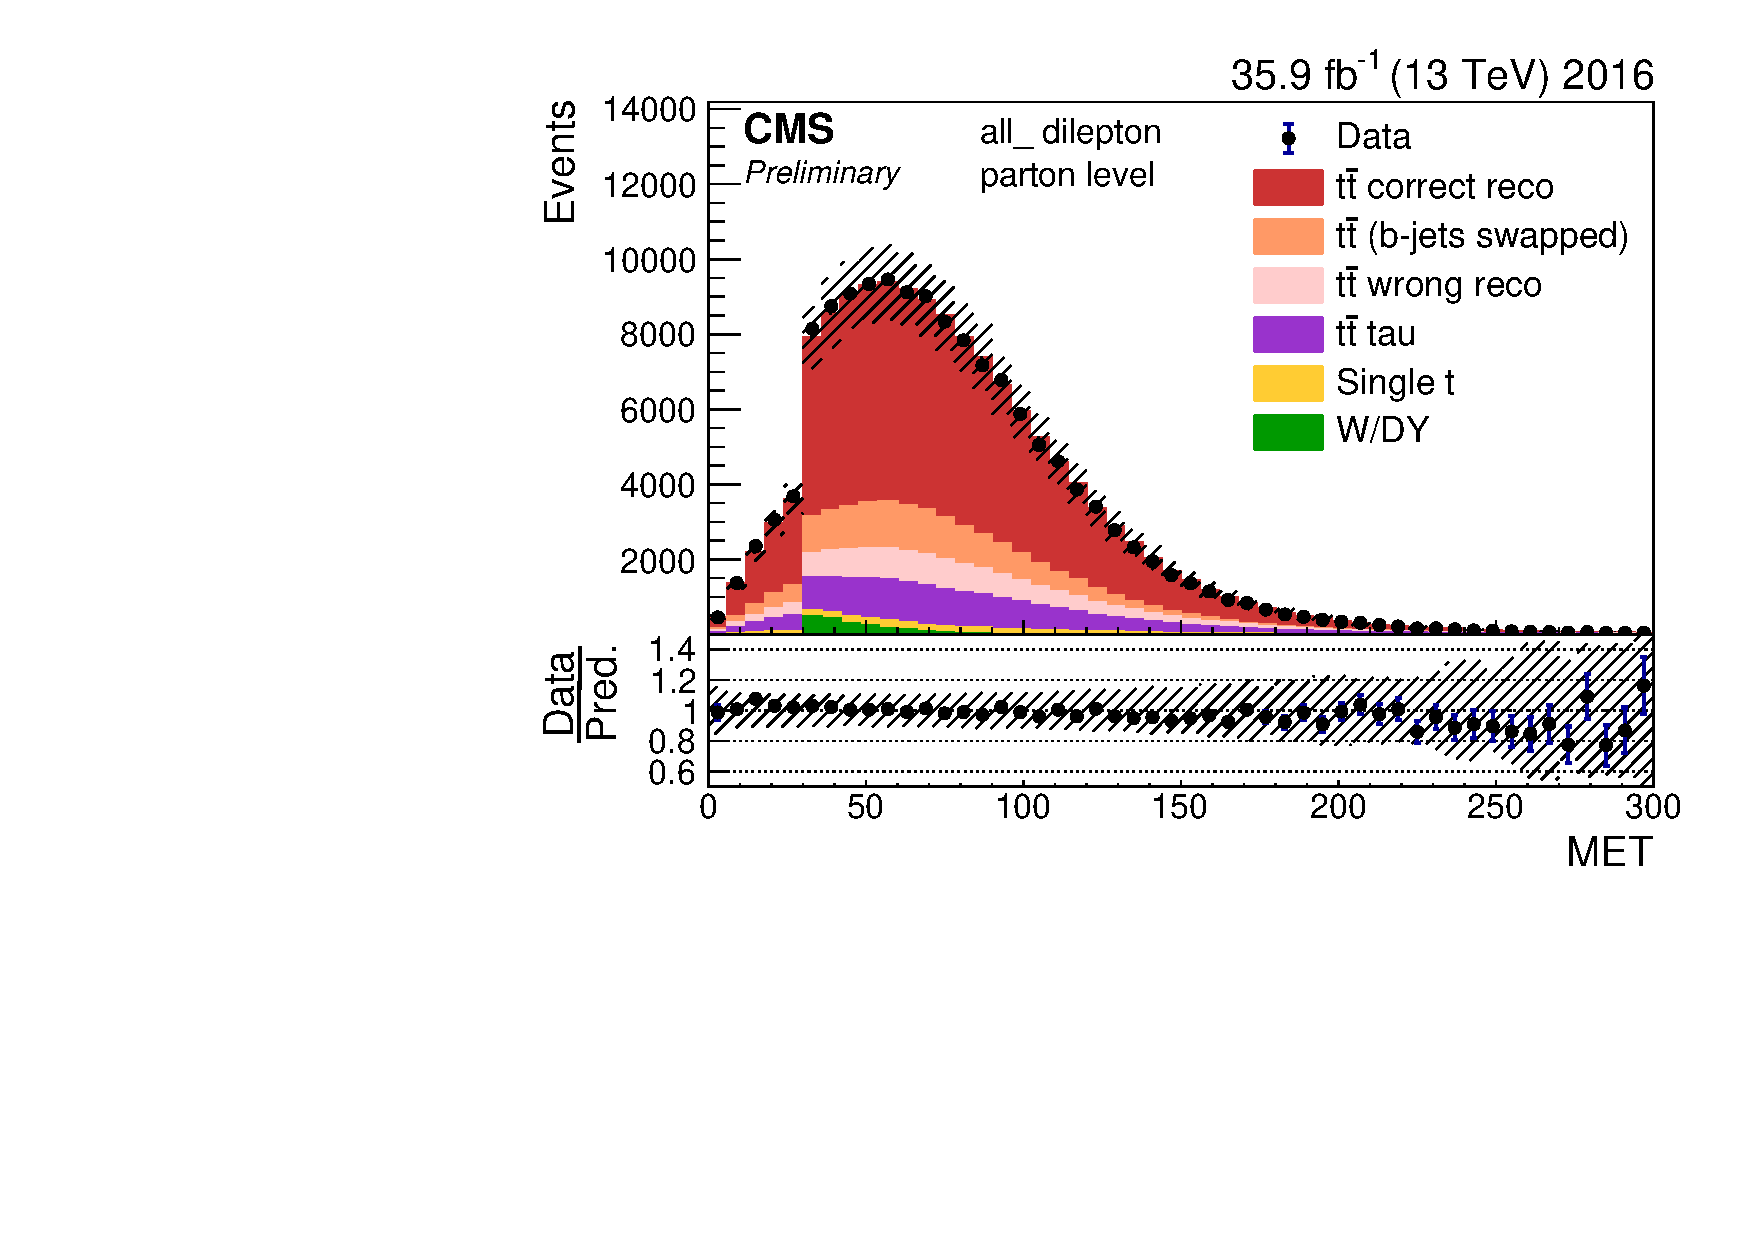
\includegraphics[width=.44\linewidth]{control/16_all_MET.pdf}
    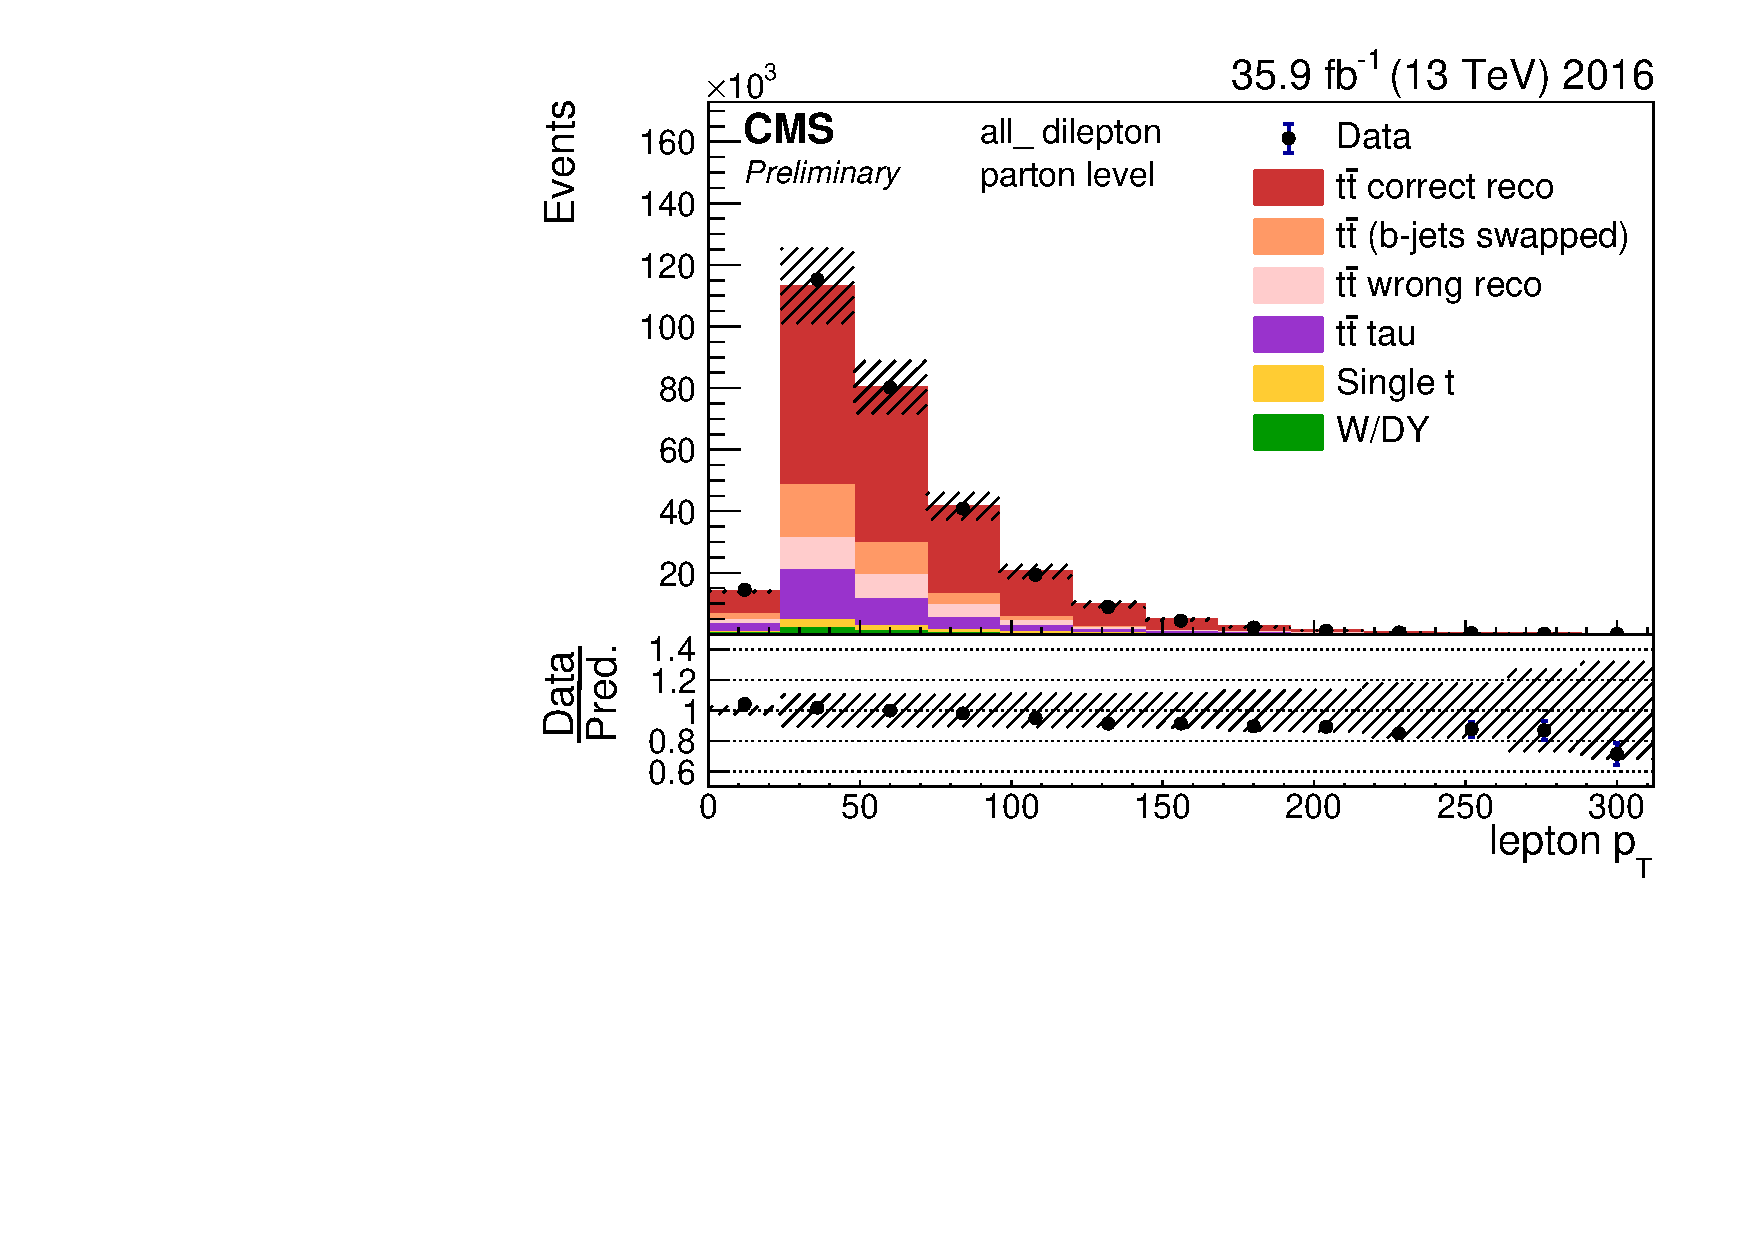
\includegraphics[width=.44\linewidth]{control/16_all_lep_pt.pdf}
    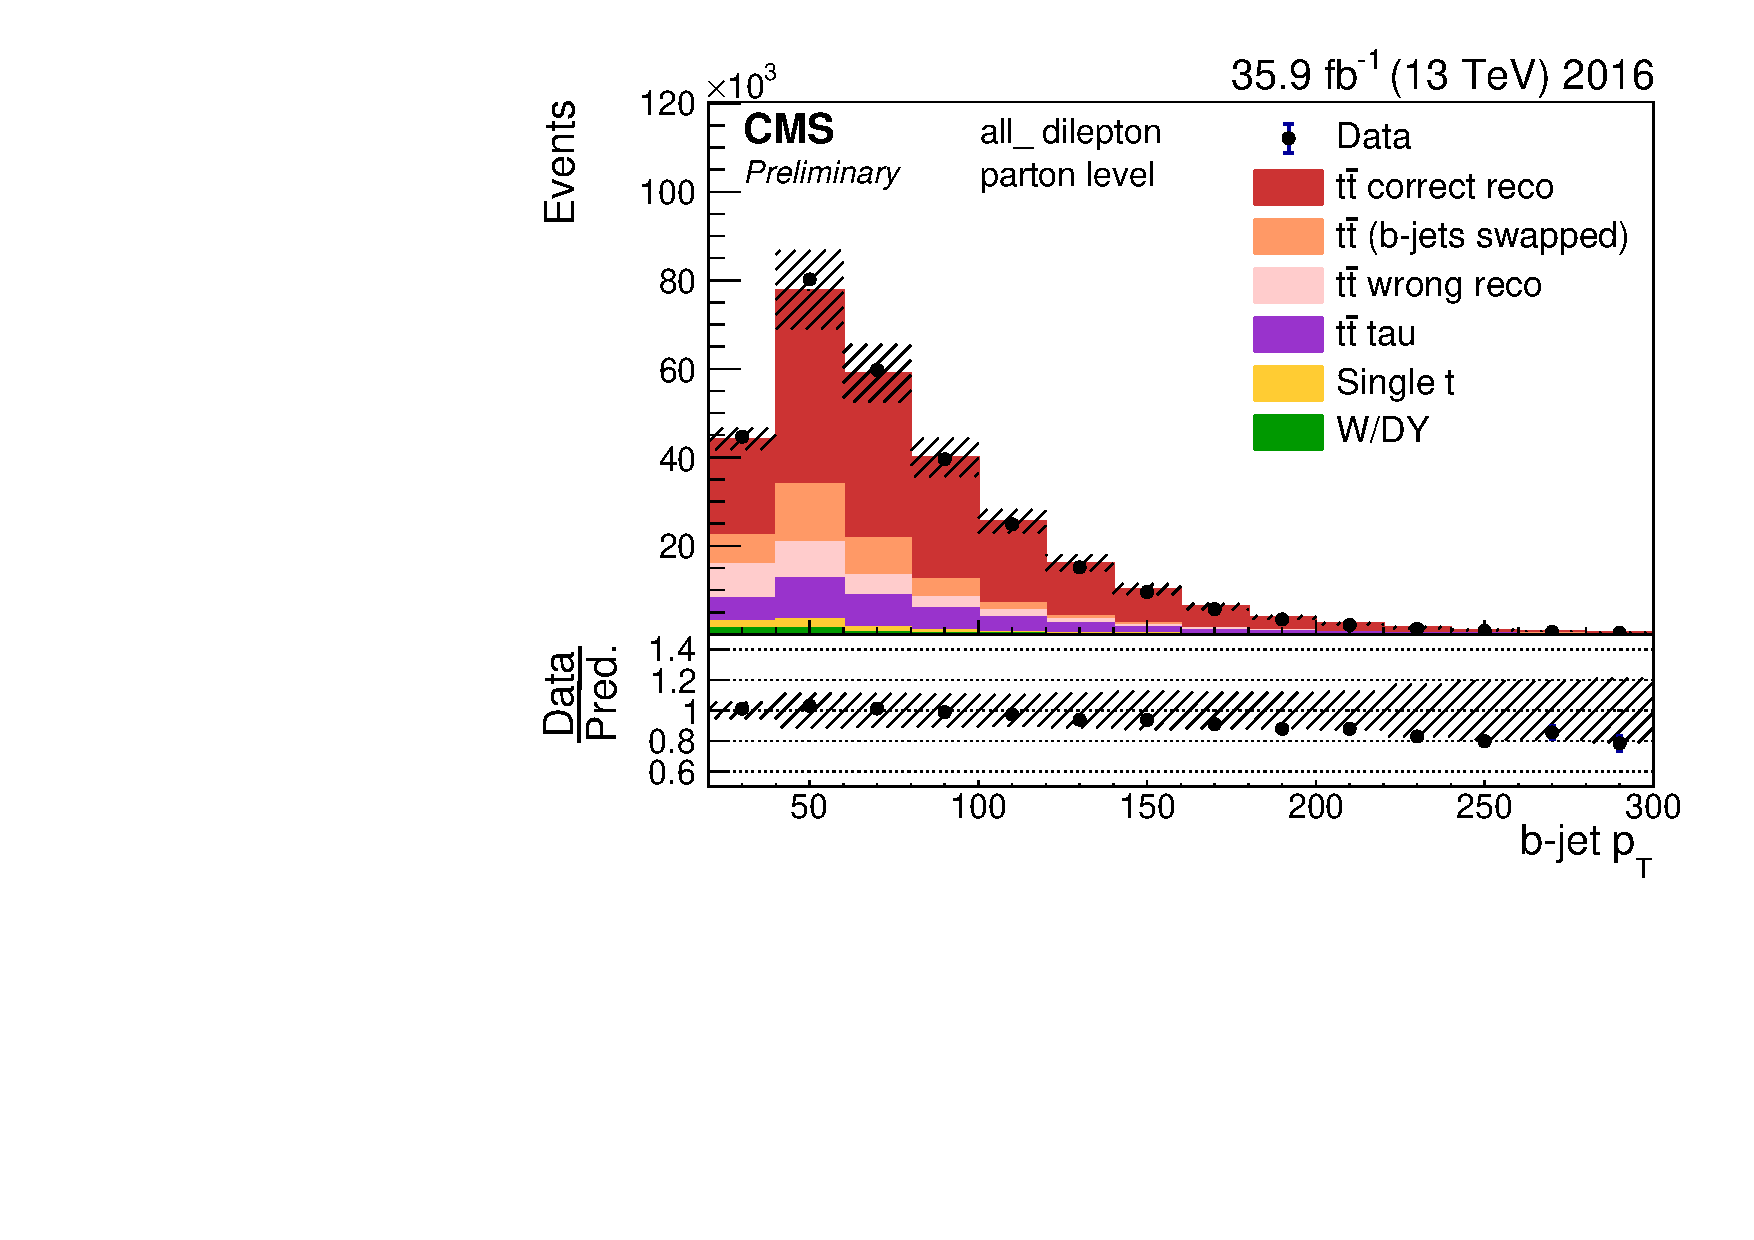
\includegraphics[width=.44\linewidth]{control/16_all_bj_Pt.pdf}
    \caption{2016 Data to MC comparison.}
    \label{fig:dmcpre_16}
\end{figure}

% \begin{figure}[h]
%     \centering
%     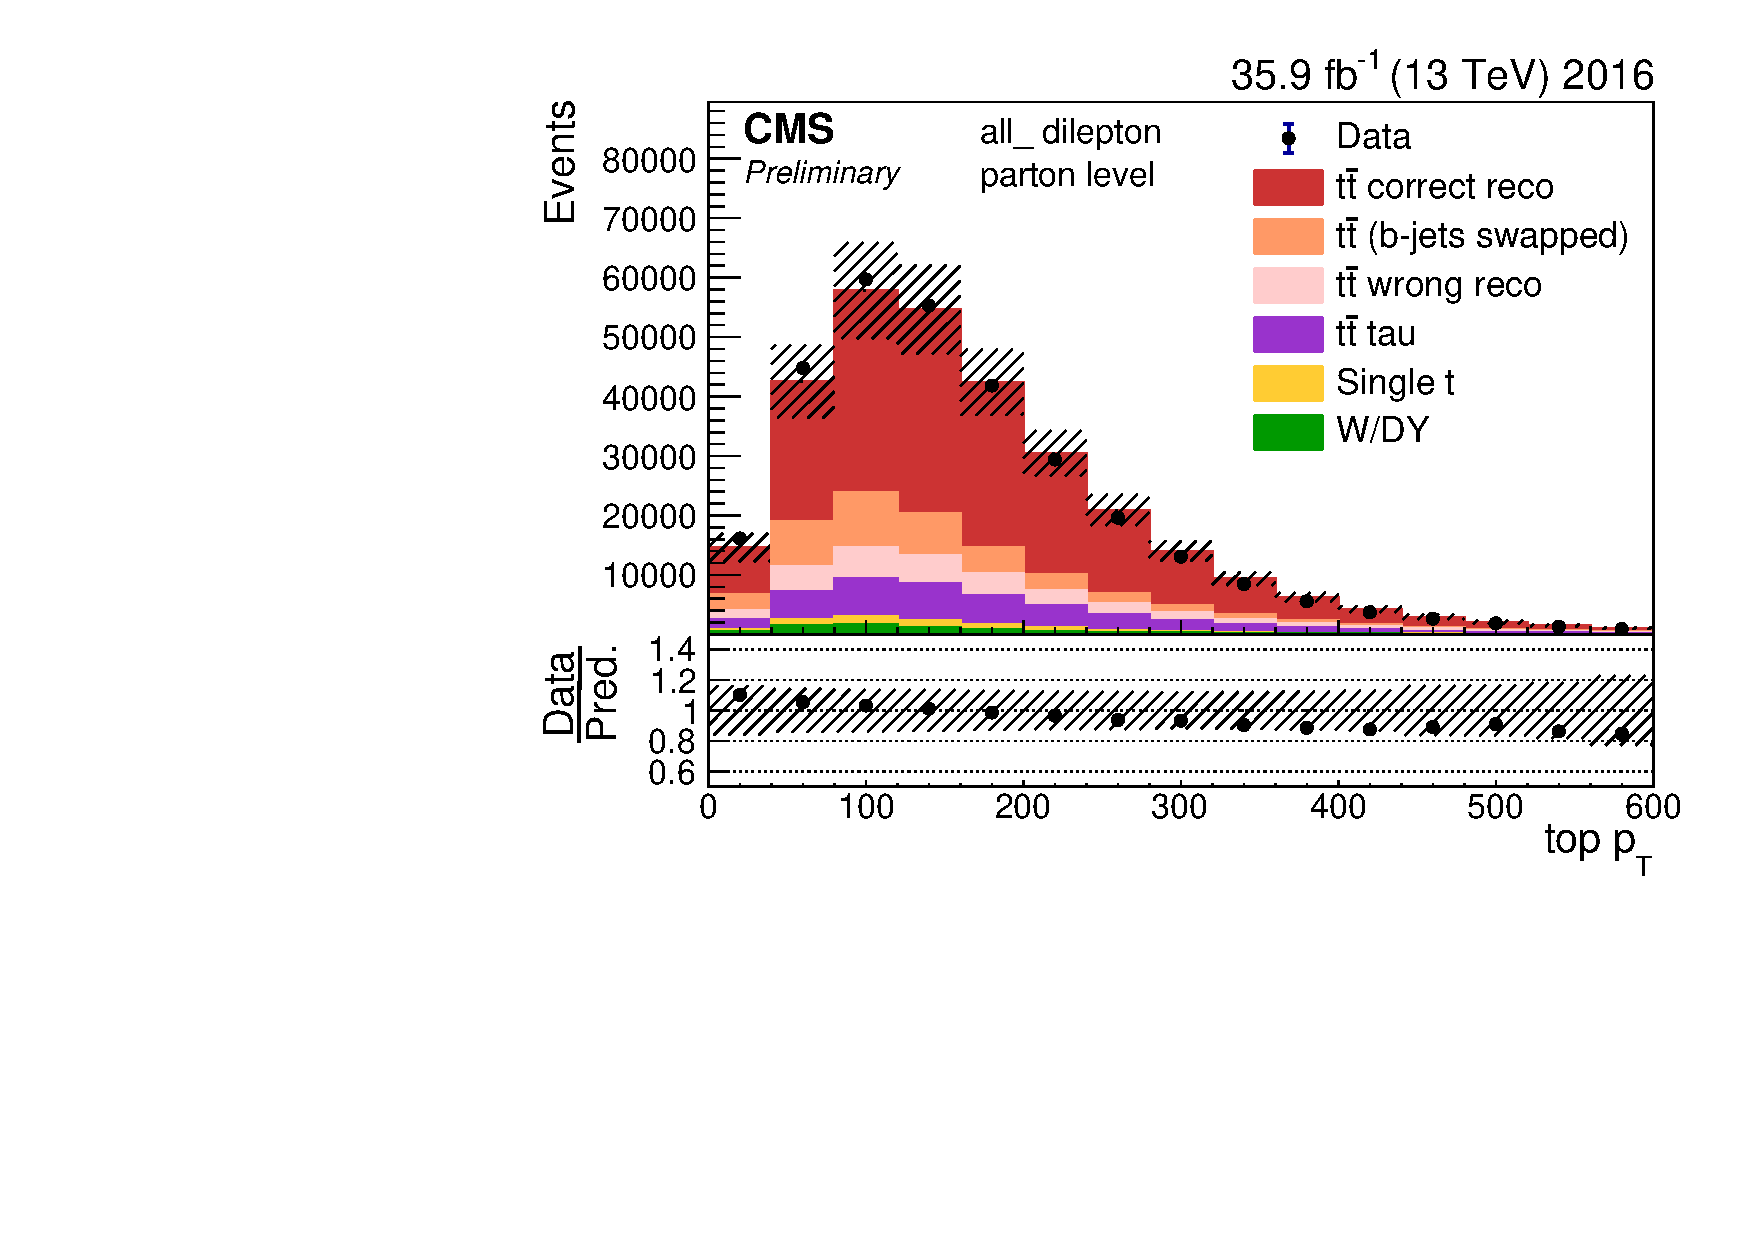
\includegraphics[width=.44\linewidth]{figs/toppt_16.pdf}
%     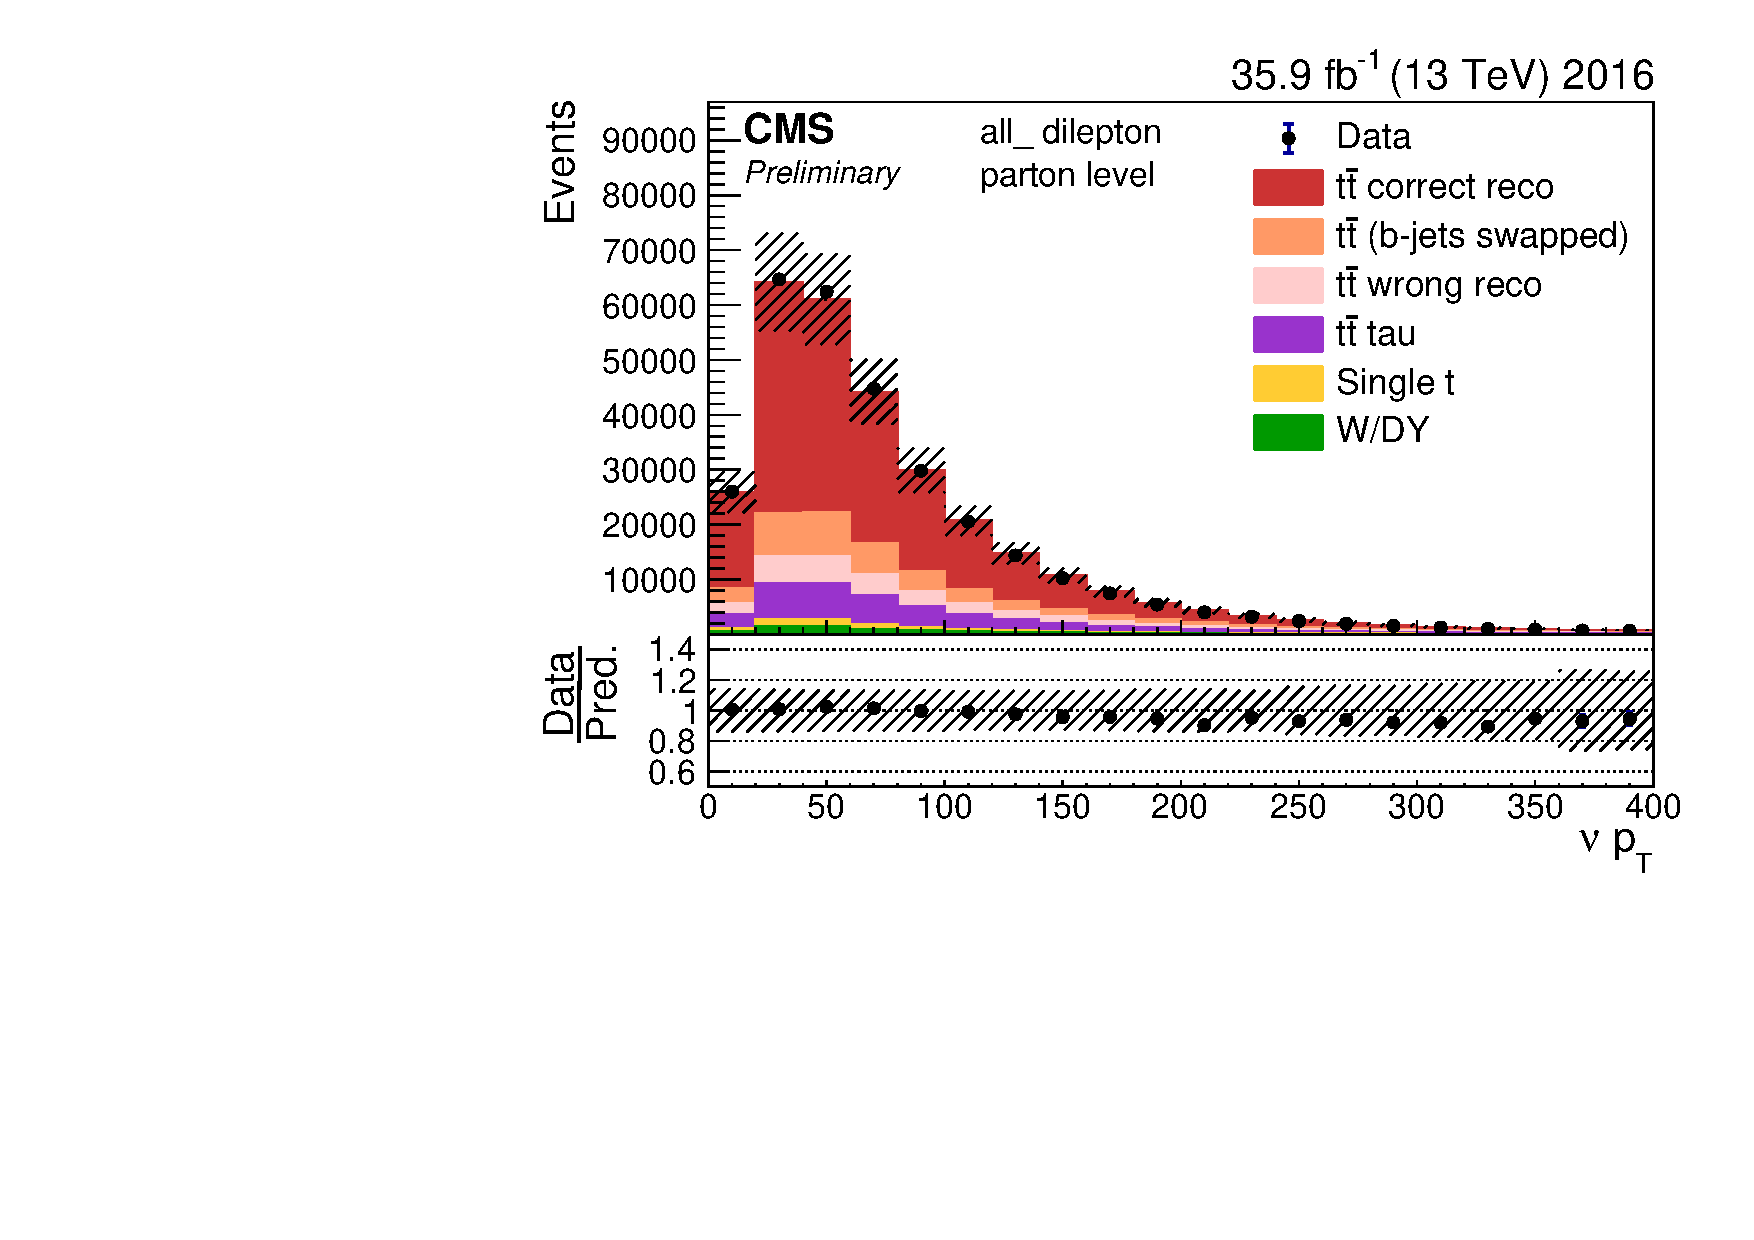
\includegraphics[width=.44\linewidth]{figs/nupt_16.pdf}
%     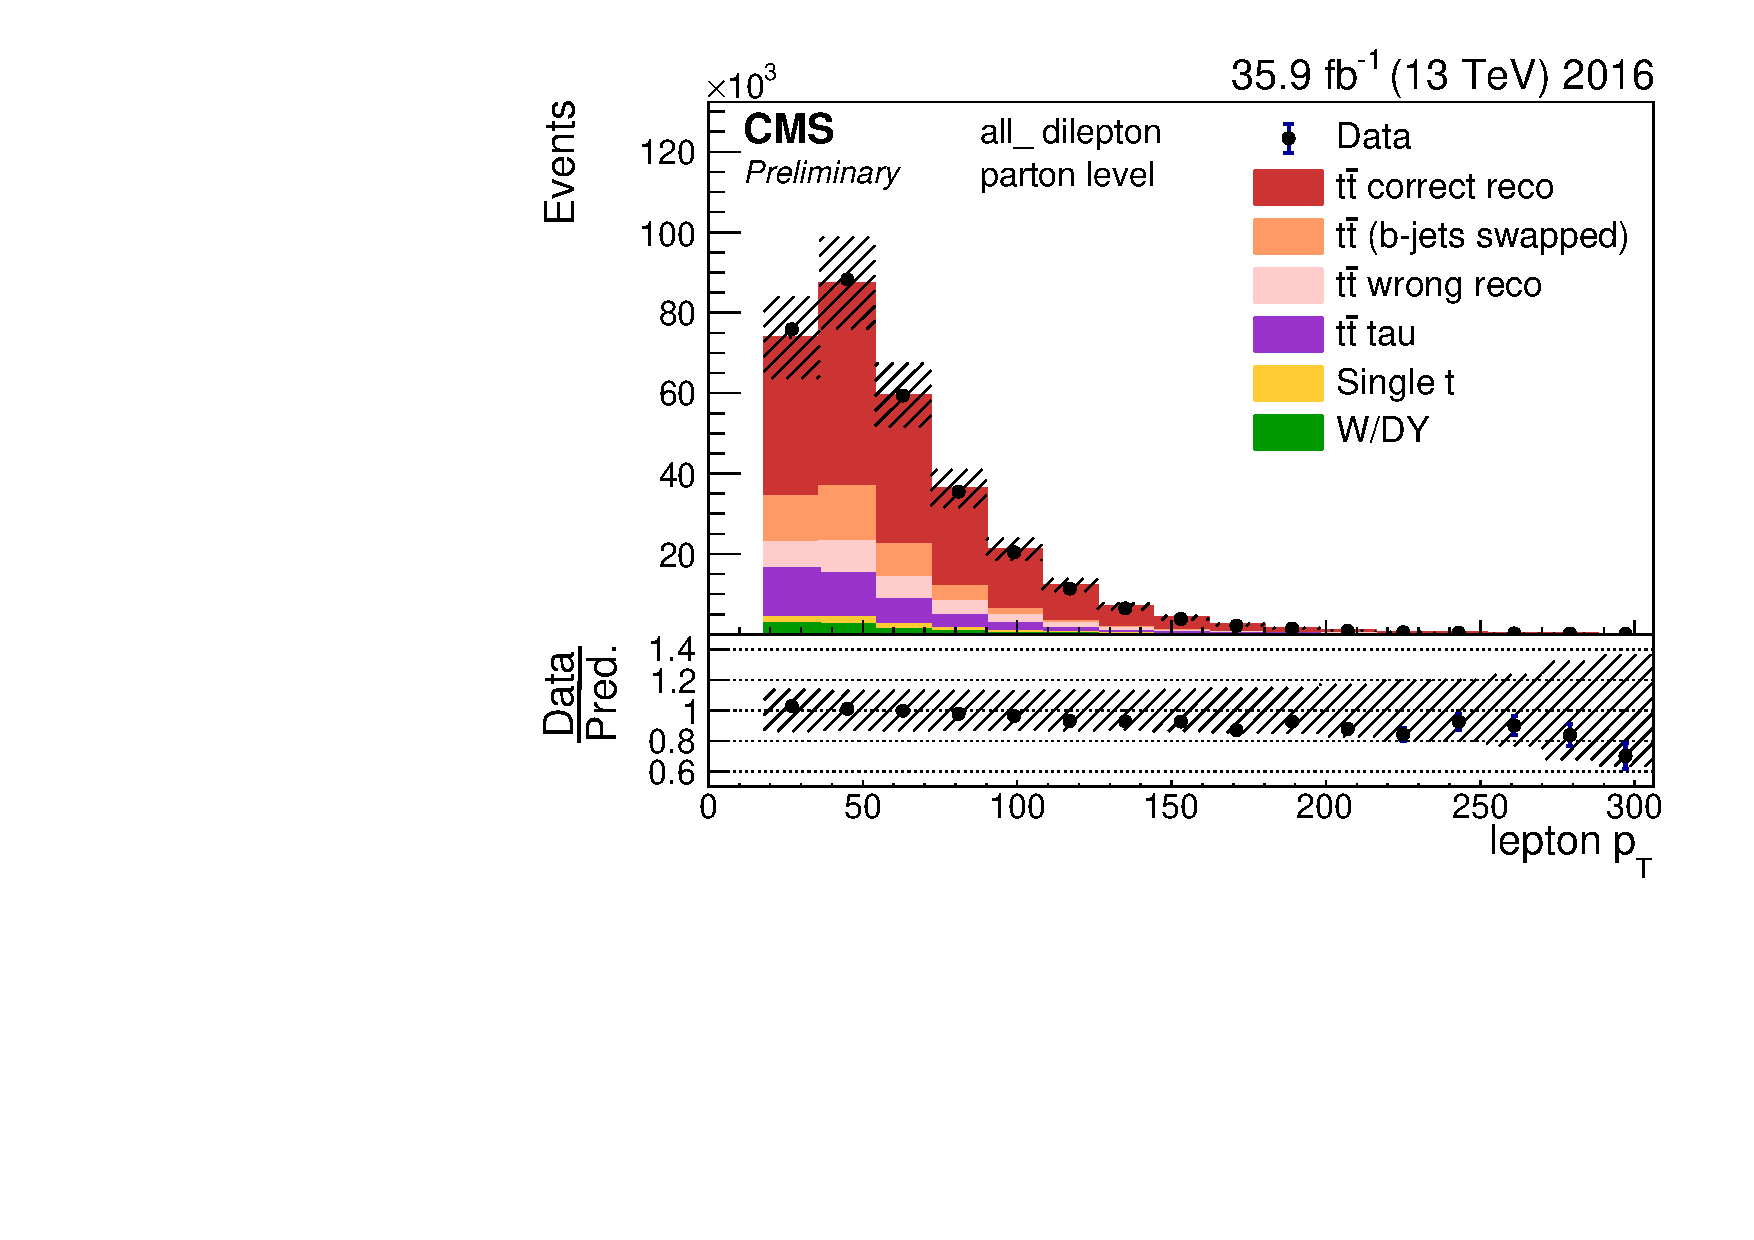
\includegraphics[width=.44\linewidth]{figs/leppt_16.pdf}
%     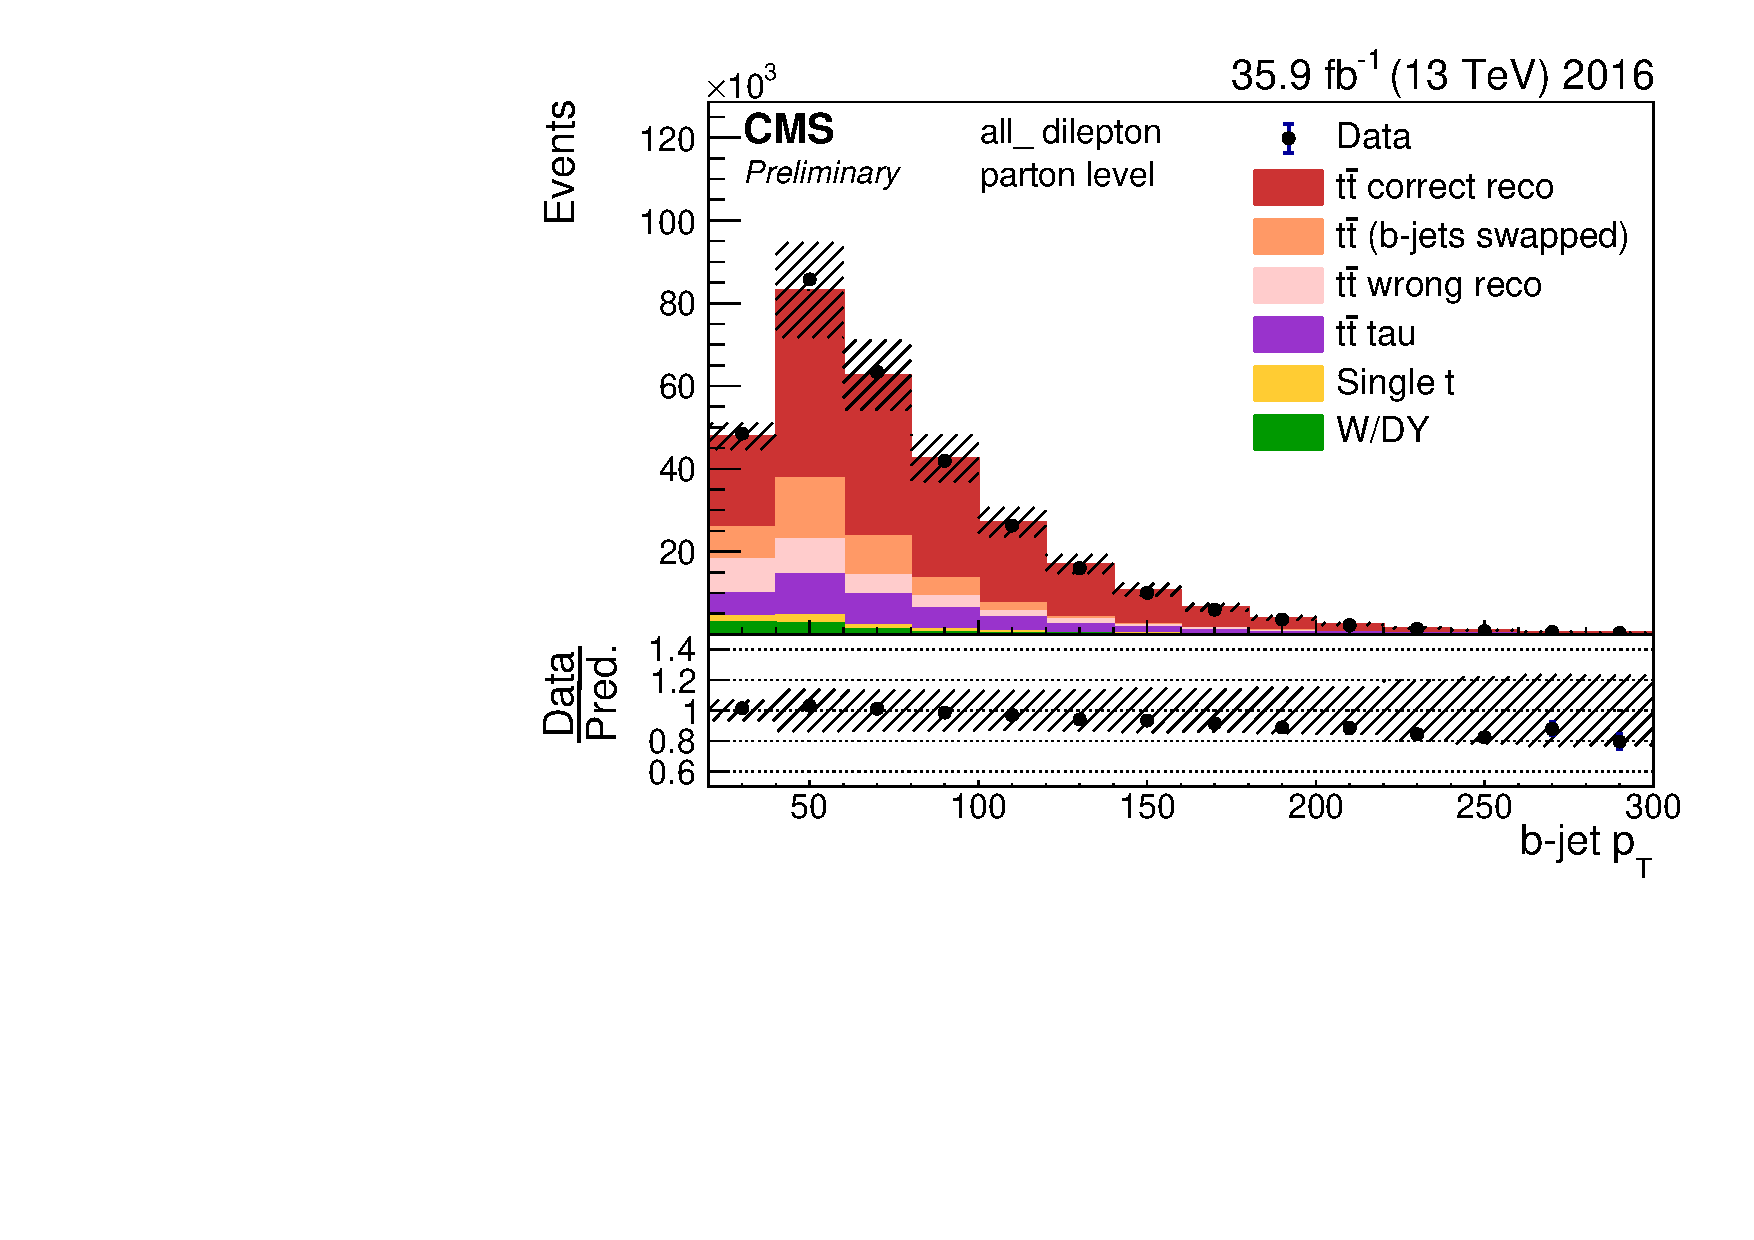
\includegraphics[width=.44\linewidth]{figs/bjpt_16.pdf}
%     \caption{2016 Data/MC agreement after neutrino/top reconstruction}
%     \label{fig:dmcpost_16}
% \end{figure}

\begin{figure}[h]
    \centering
    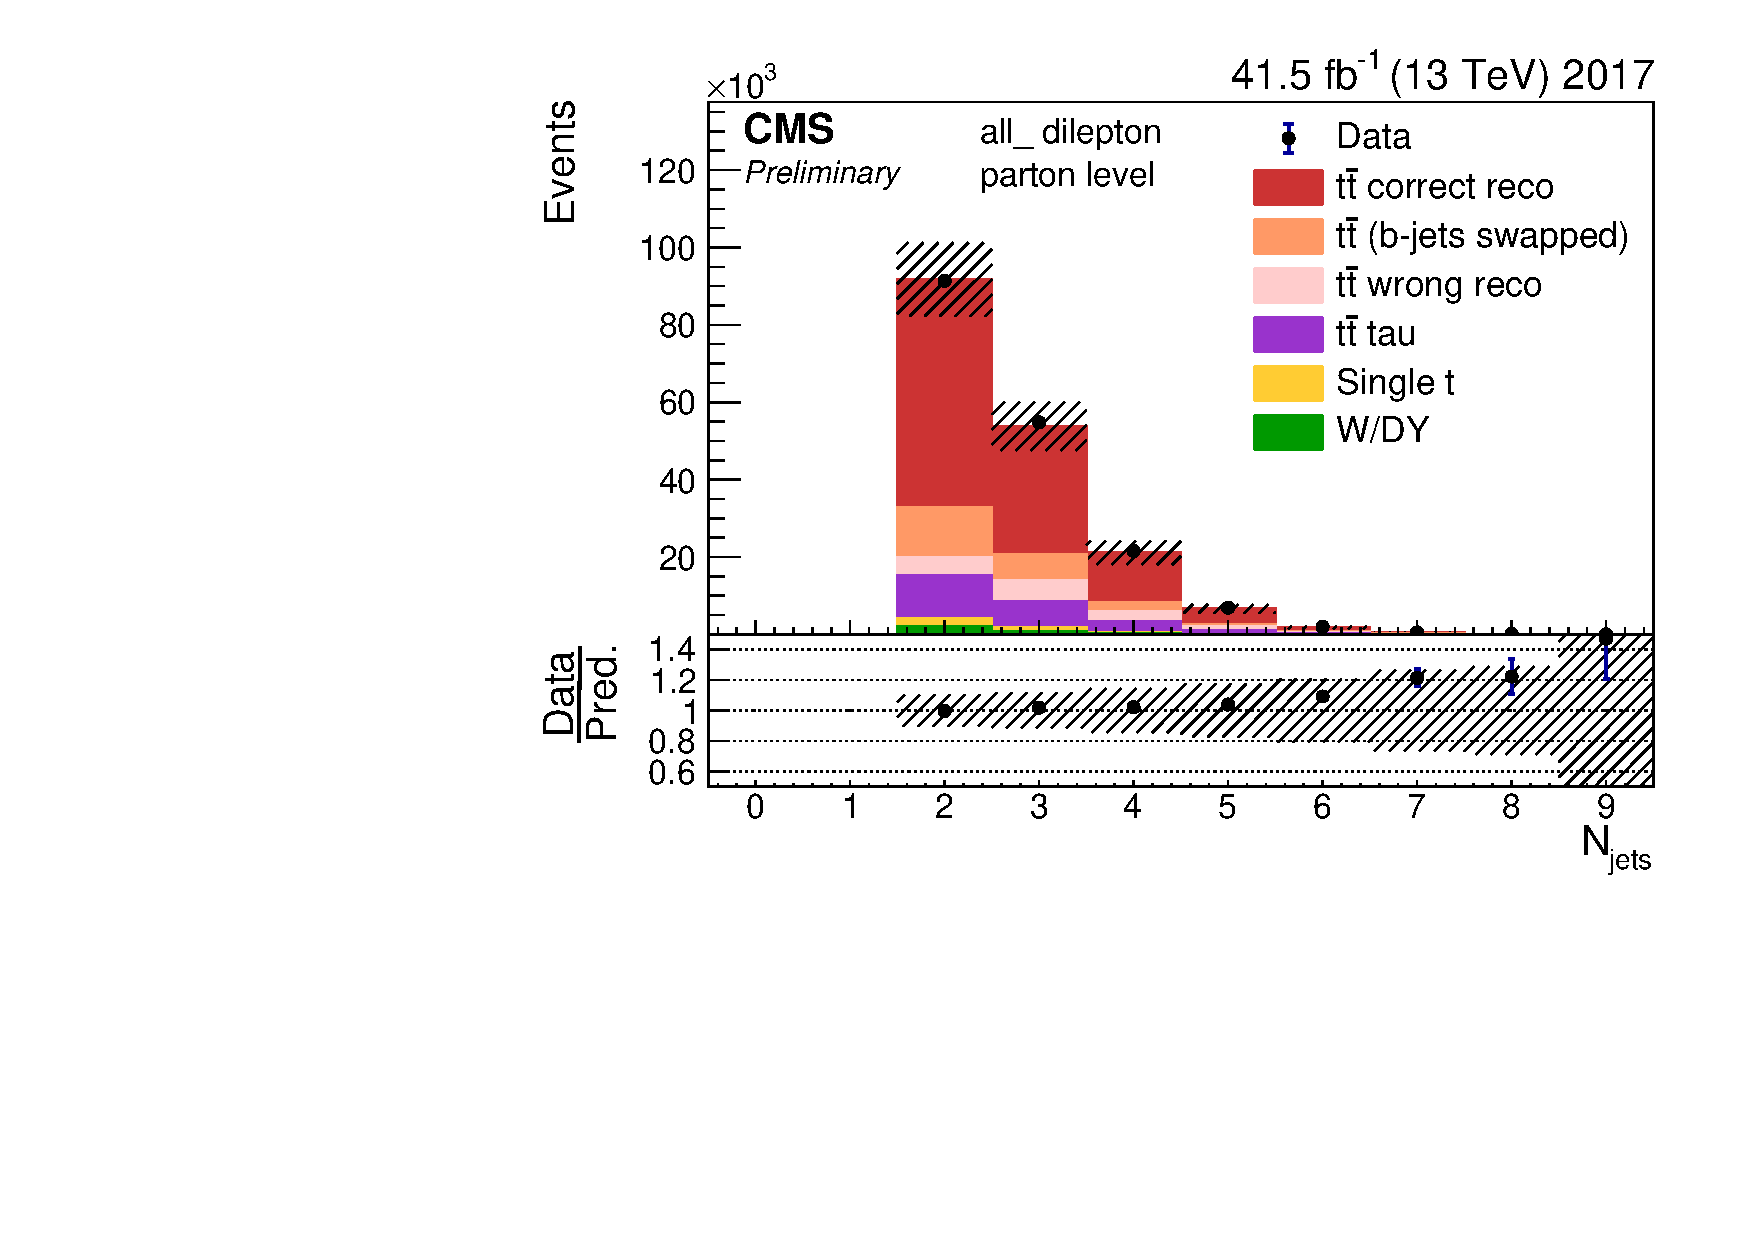
\includegraphics[width=.44\linewidth]{control/17_all_Njets.pdf}
    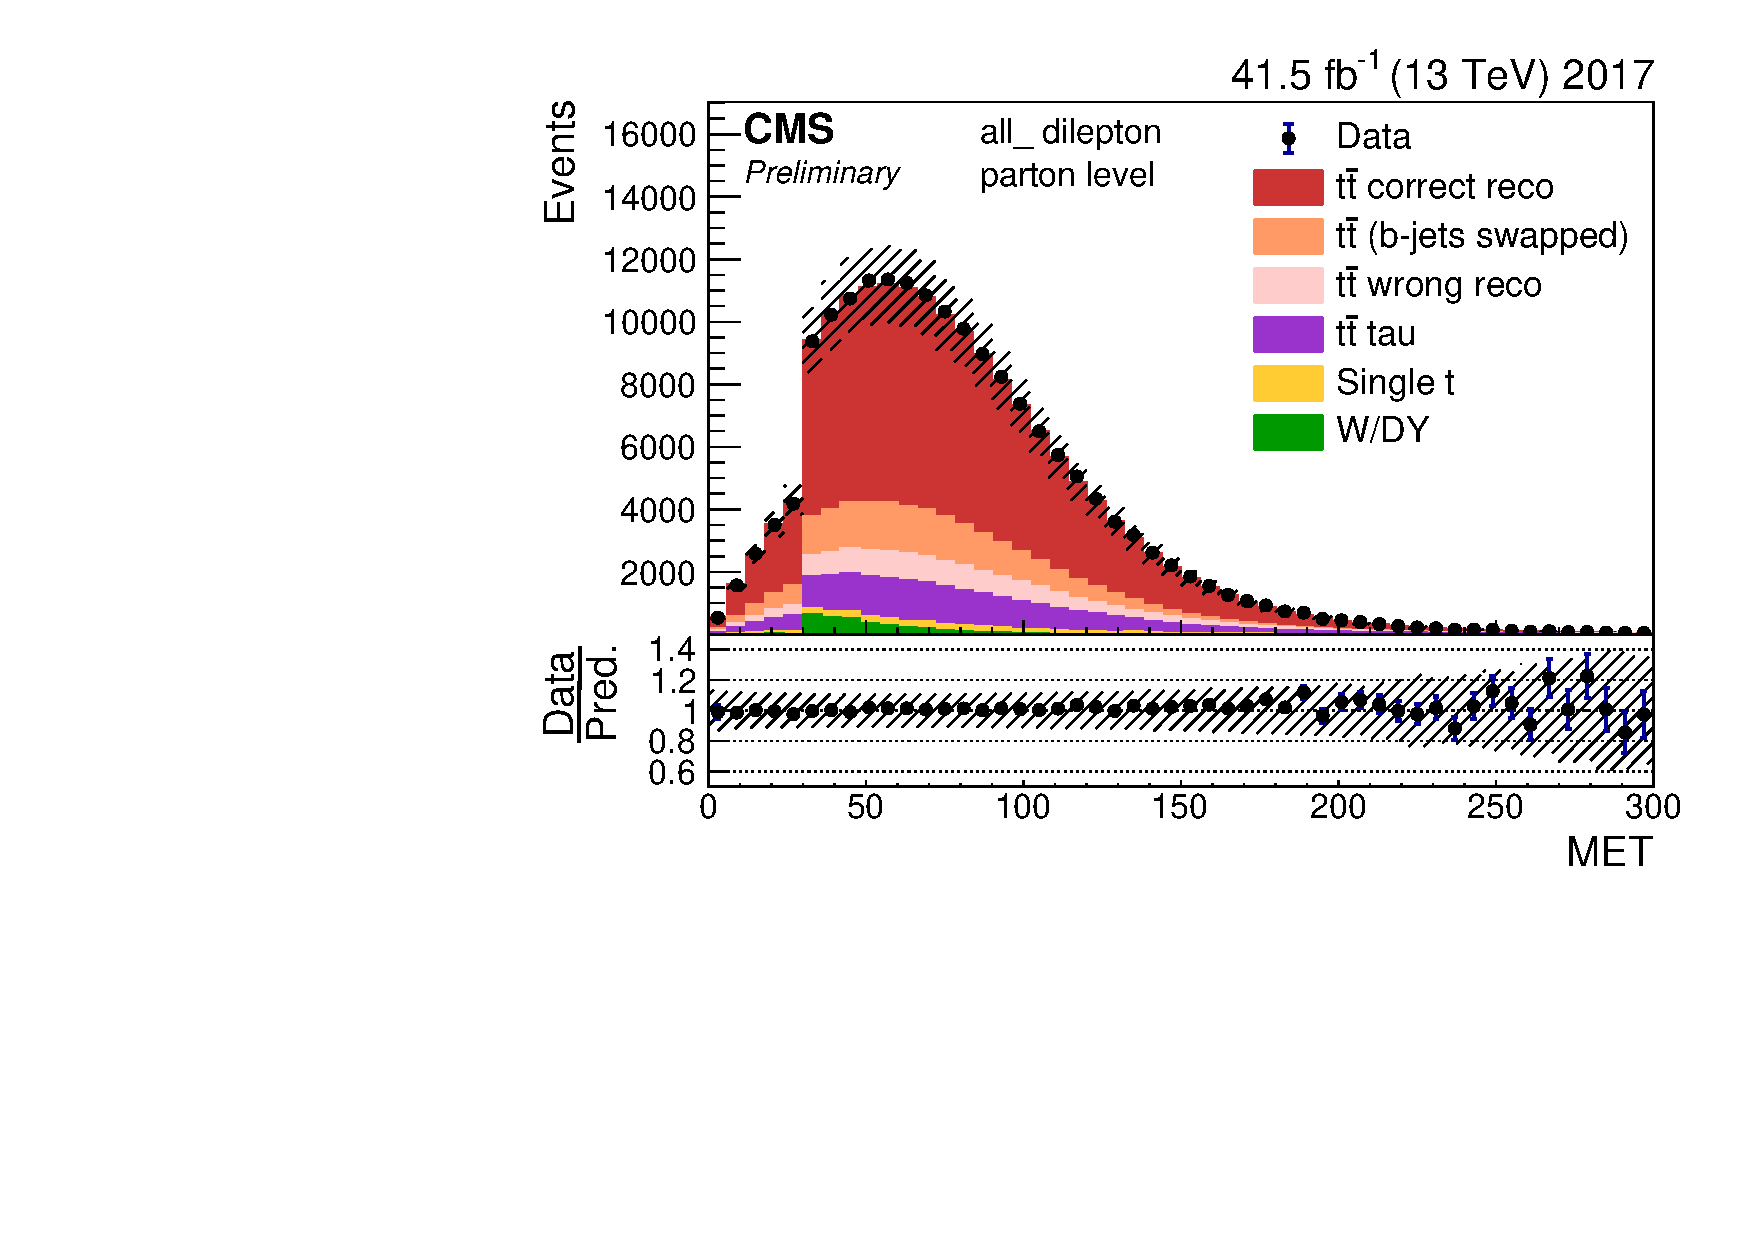
\includegraphics[width=.44\linewidth]{control/17_all_MET.pdf}
    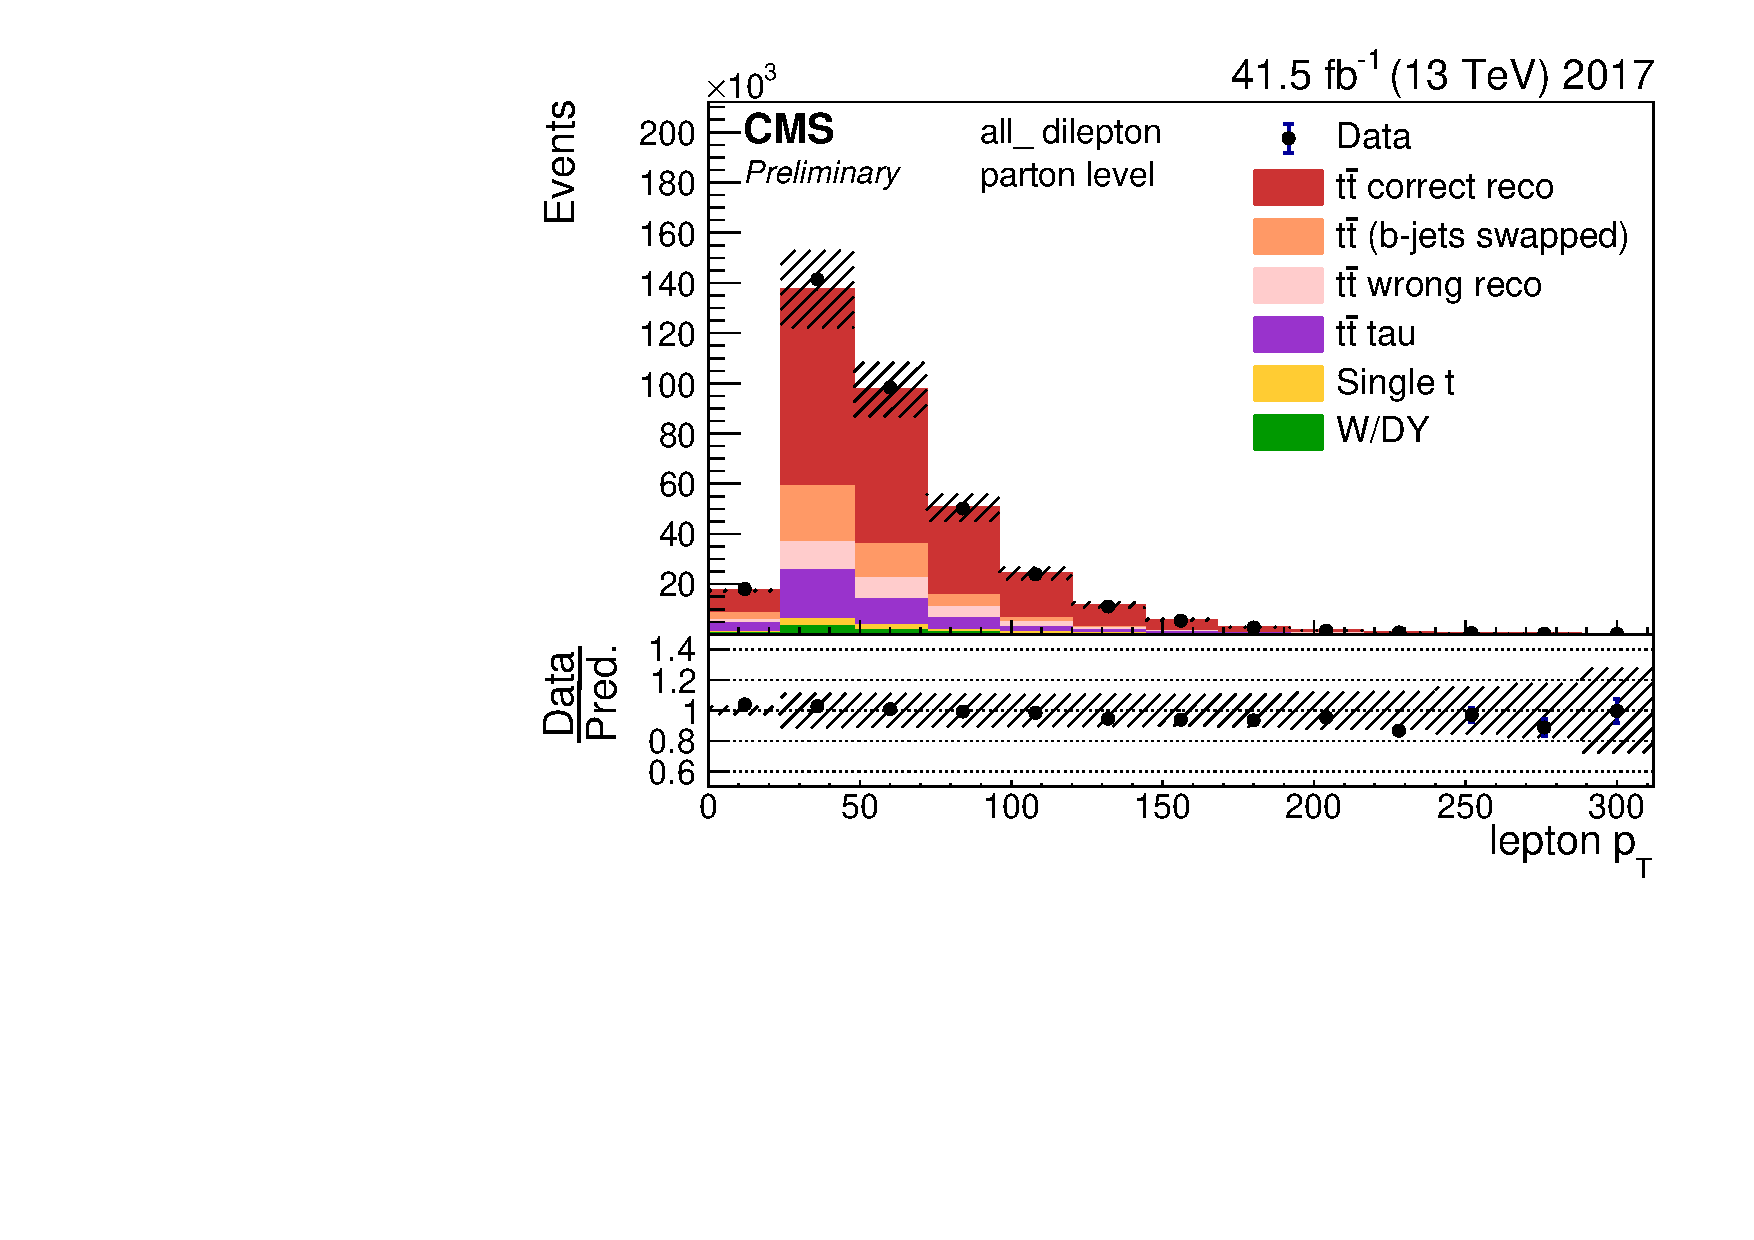
\includegraphics[width=.44\linewidth]{control/17_all_lep_pt.pdf}
    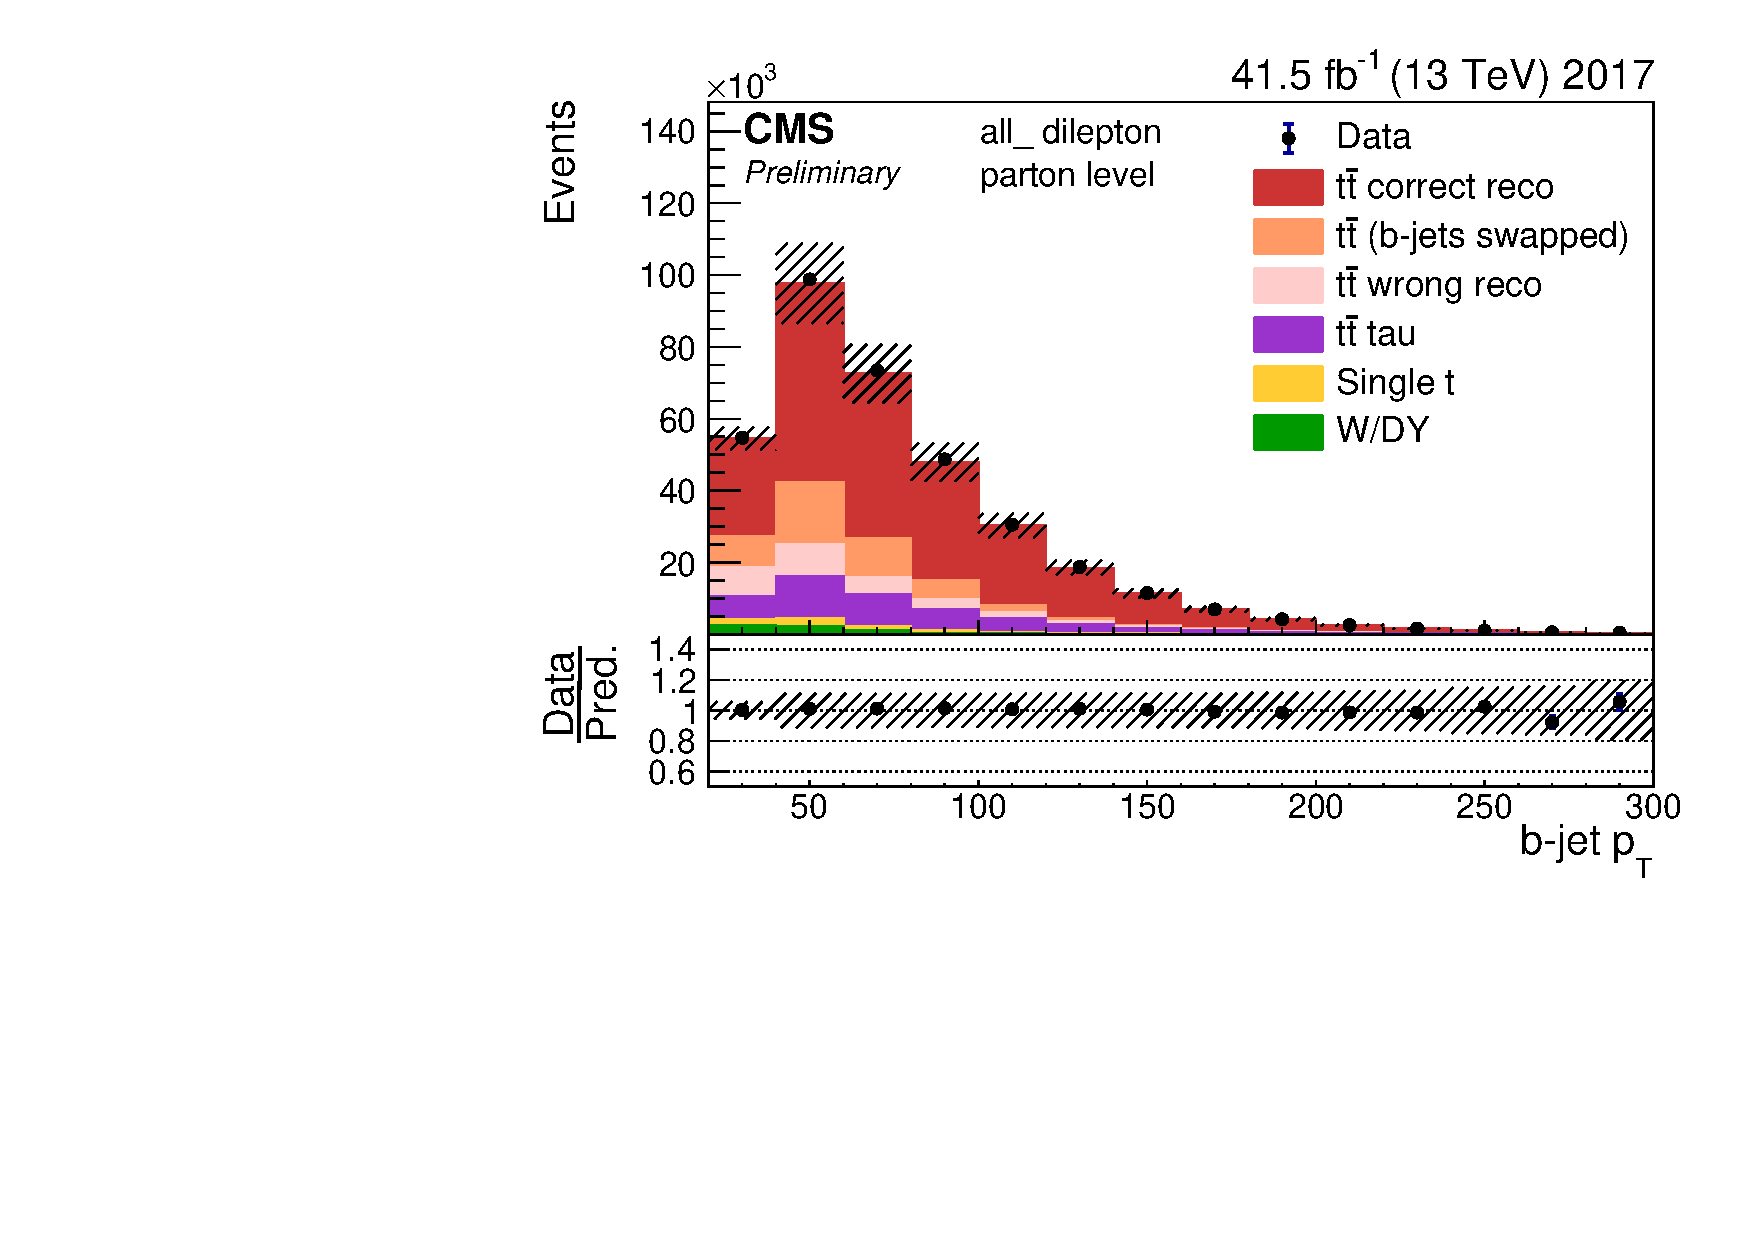
\includegraphics[width=.44\linewidth]{control/17_all_bj_Pt.pdf}
    \caption{2017 Data to MC comparison. }
    \label{fig:dmcpre_17}
\end{figure}

% \begin{figure}[h]
%     \centering
%     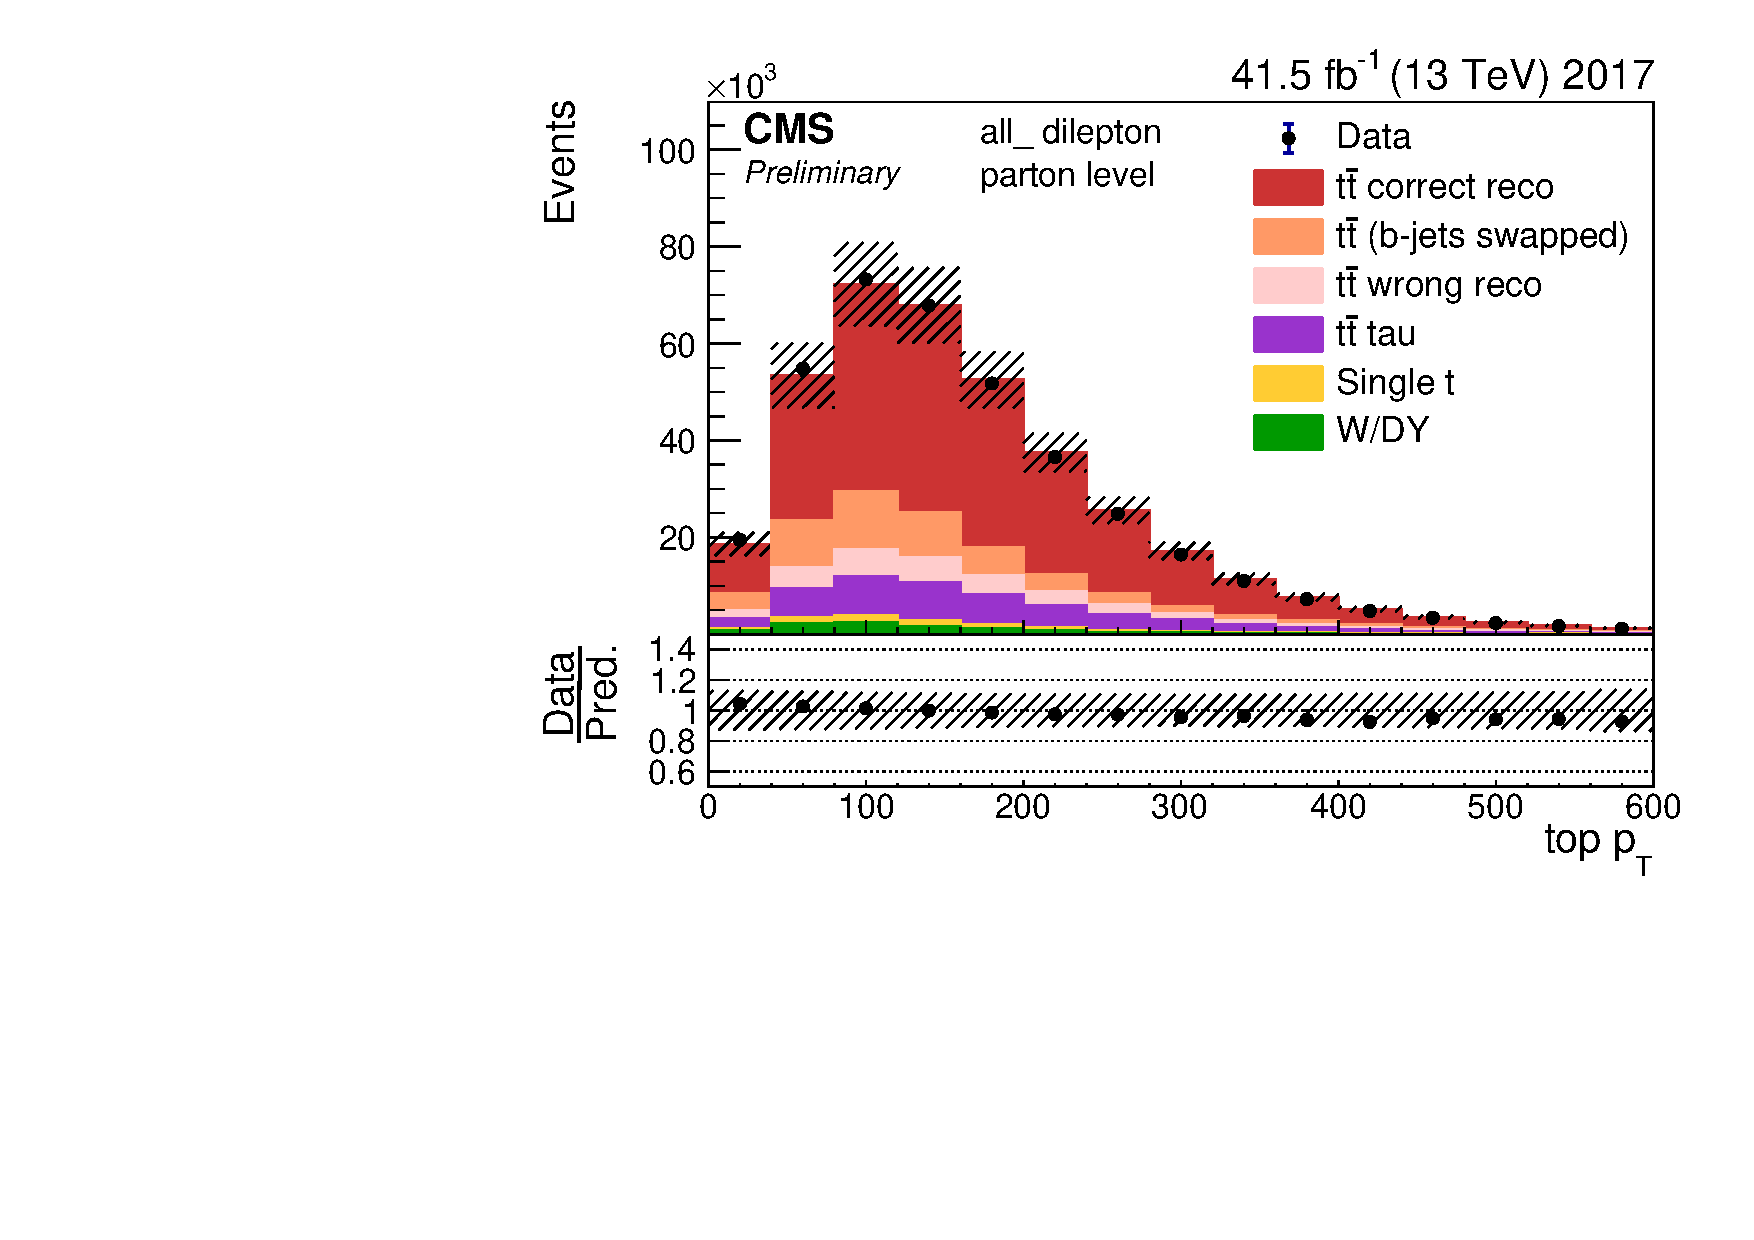
\includegraphics[width=.44\linewidth]{figs/toppt_17.pdf}
%     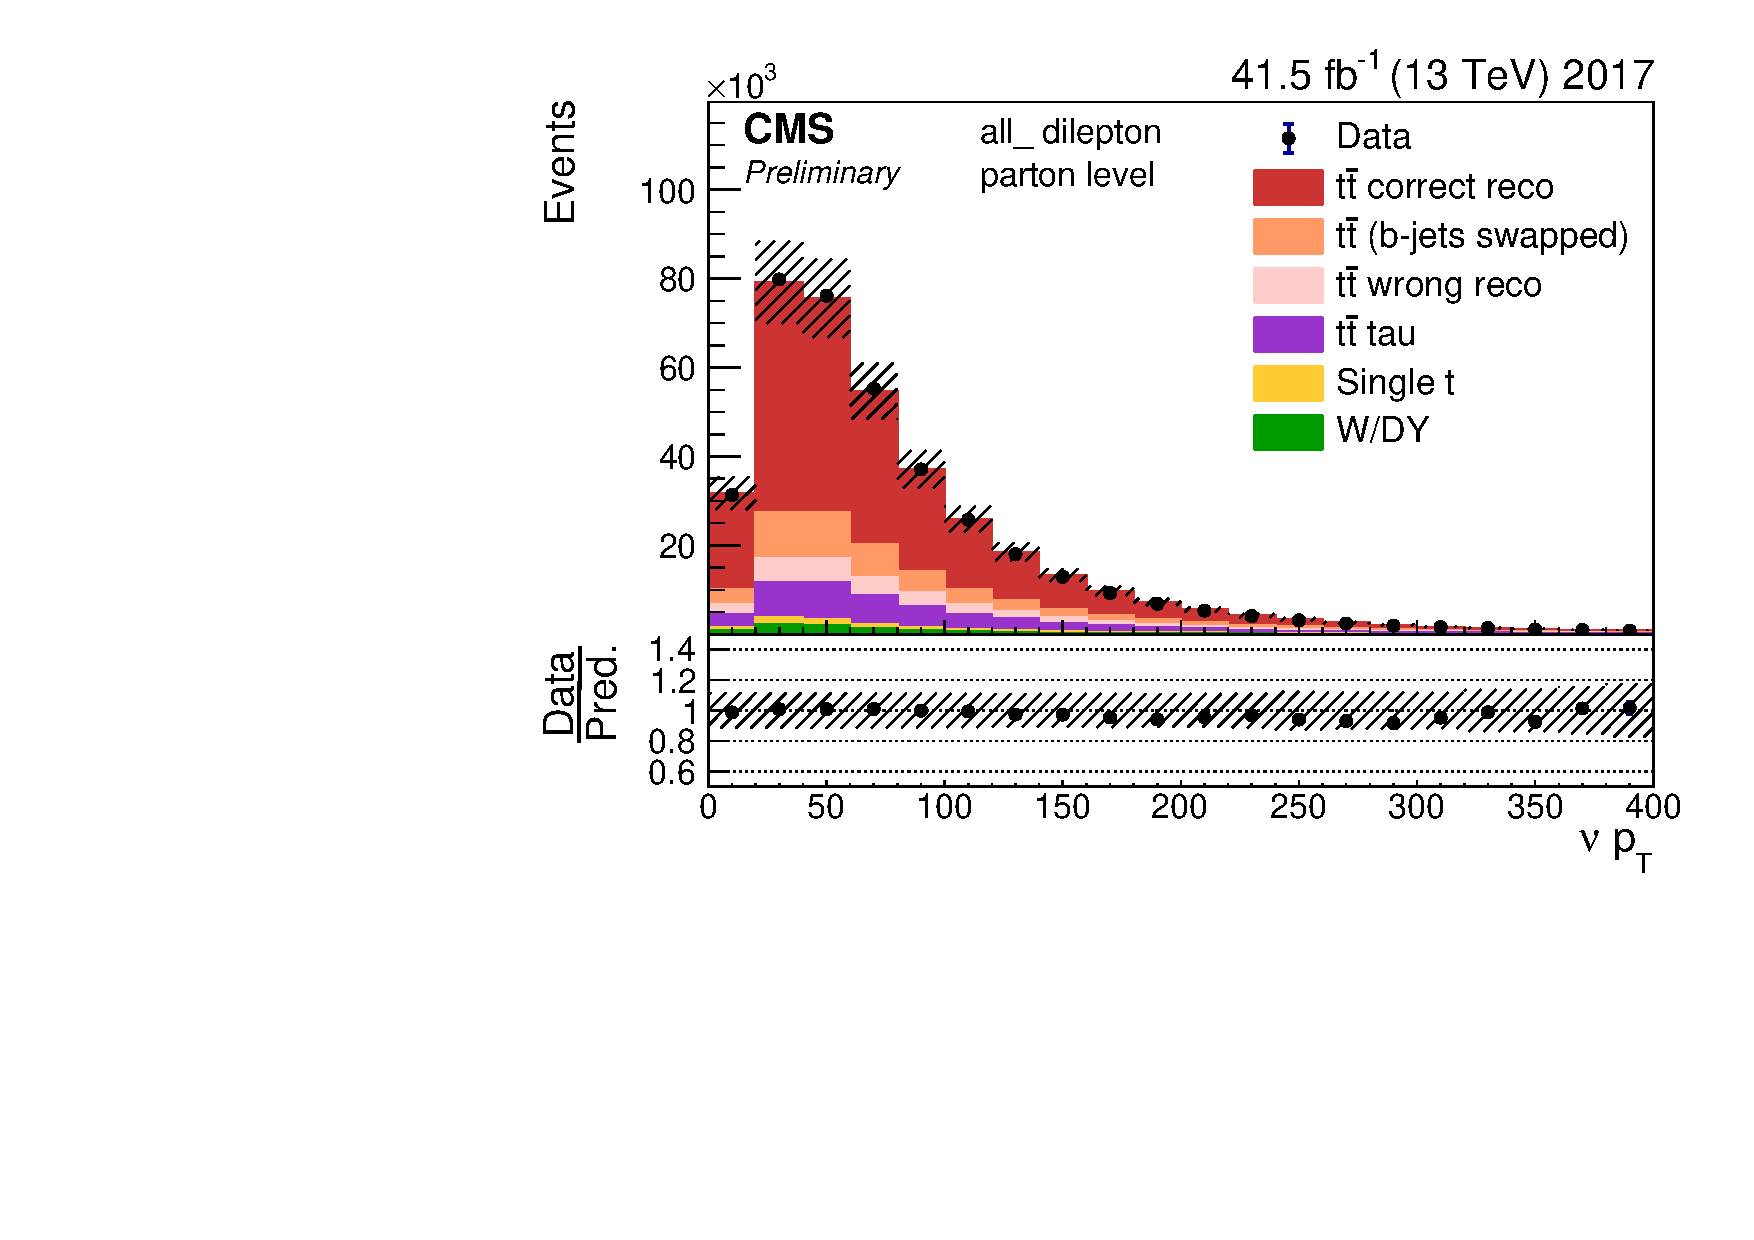
\includegraphics[width=.44\linewidth]{figs/nupt_17.pdf}
%     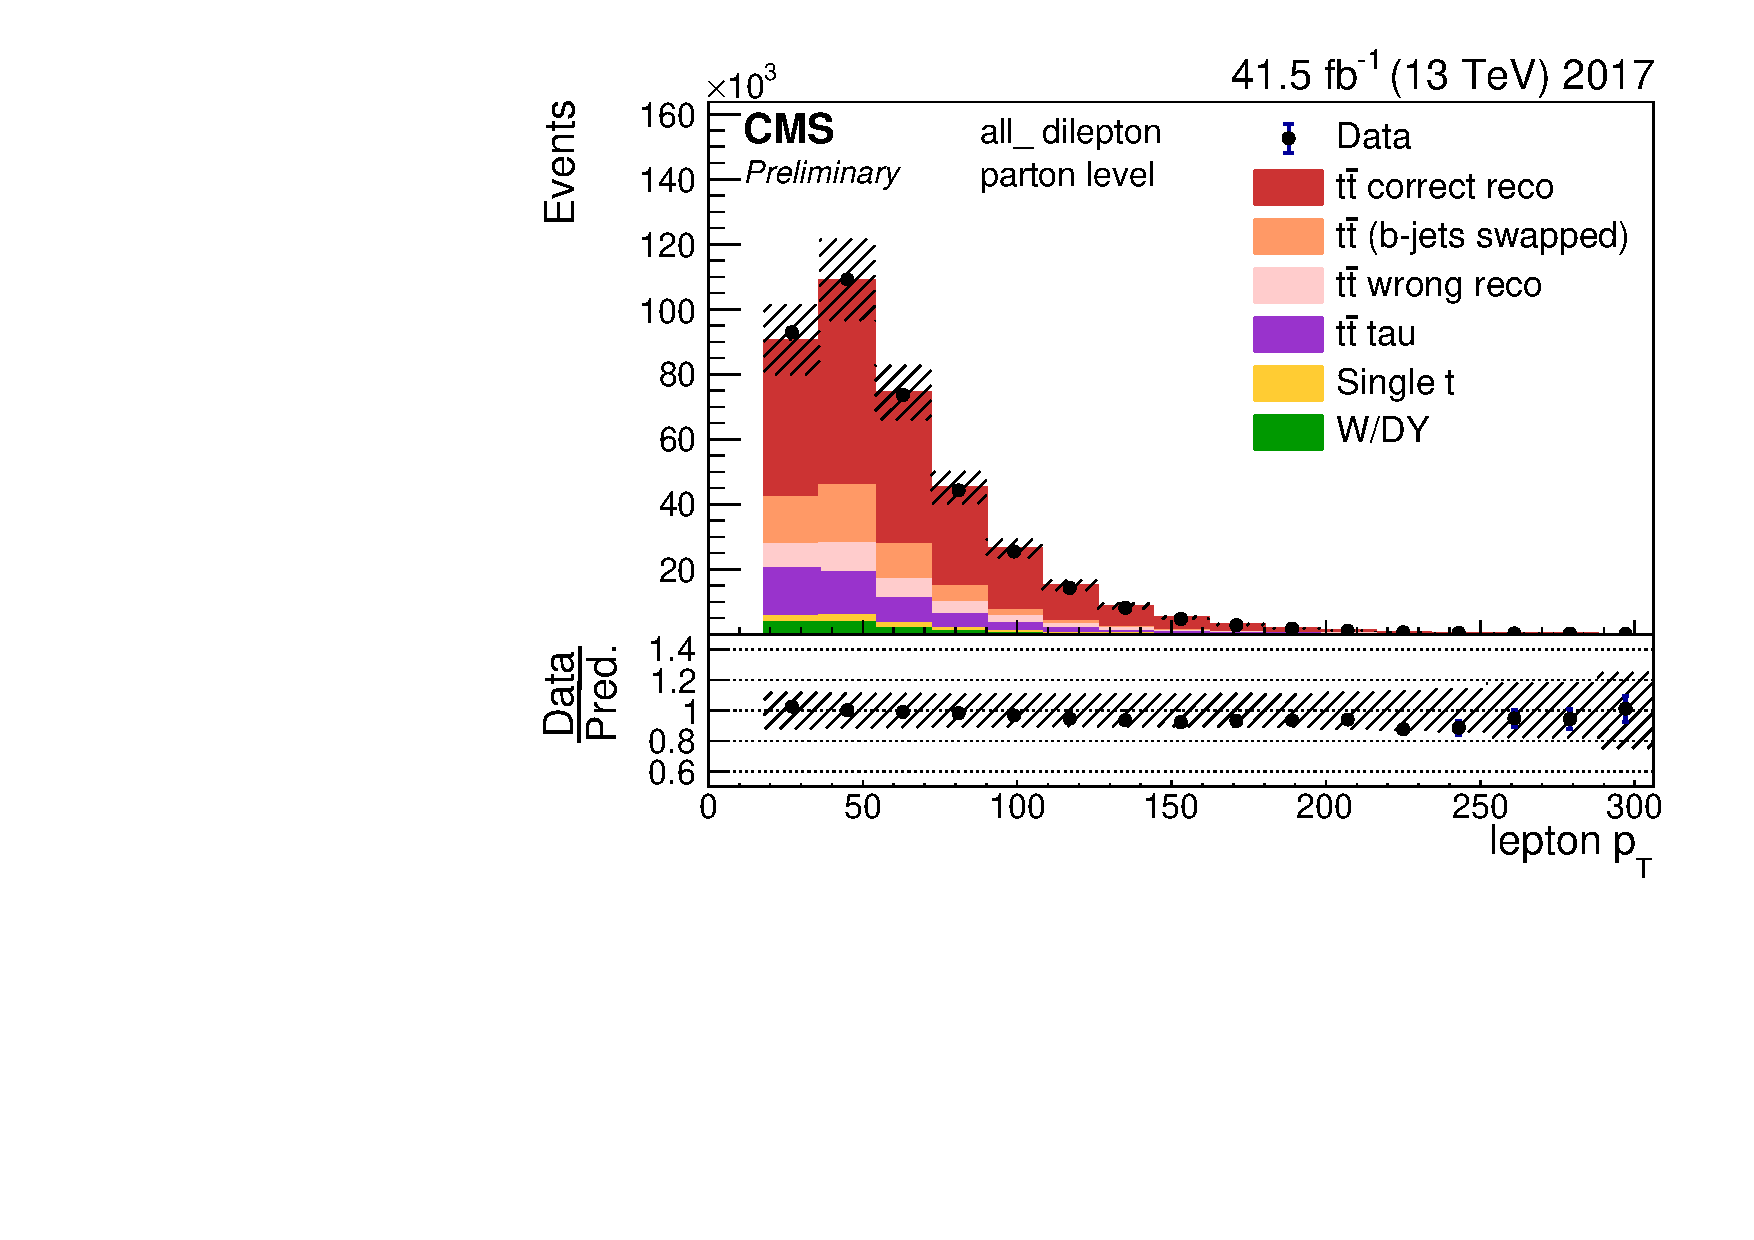
\includegraphics[width=.44\linewidth]{figs/leppt_17.pdf}
%     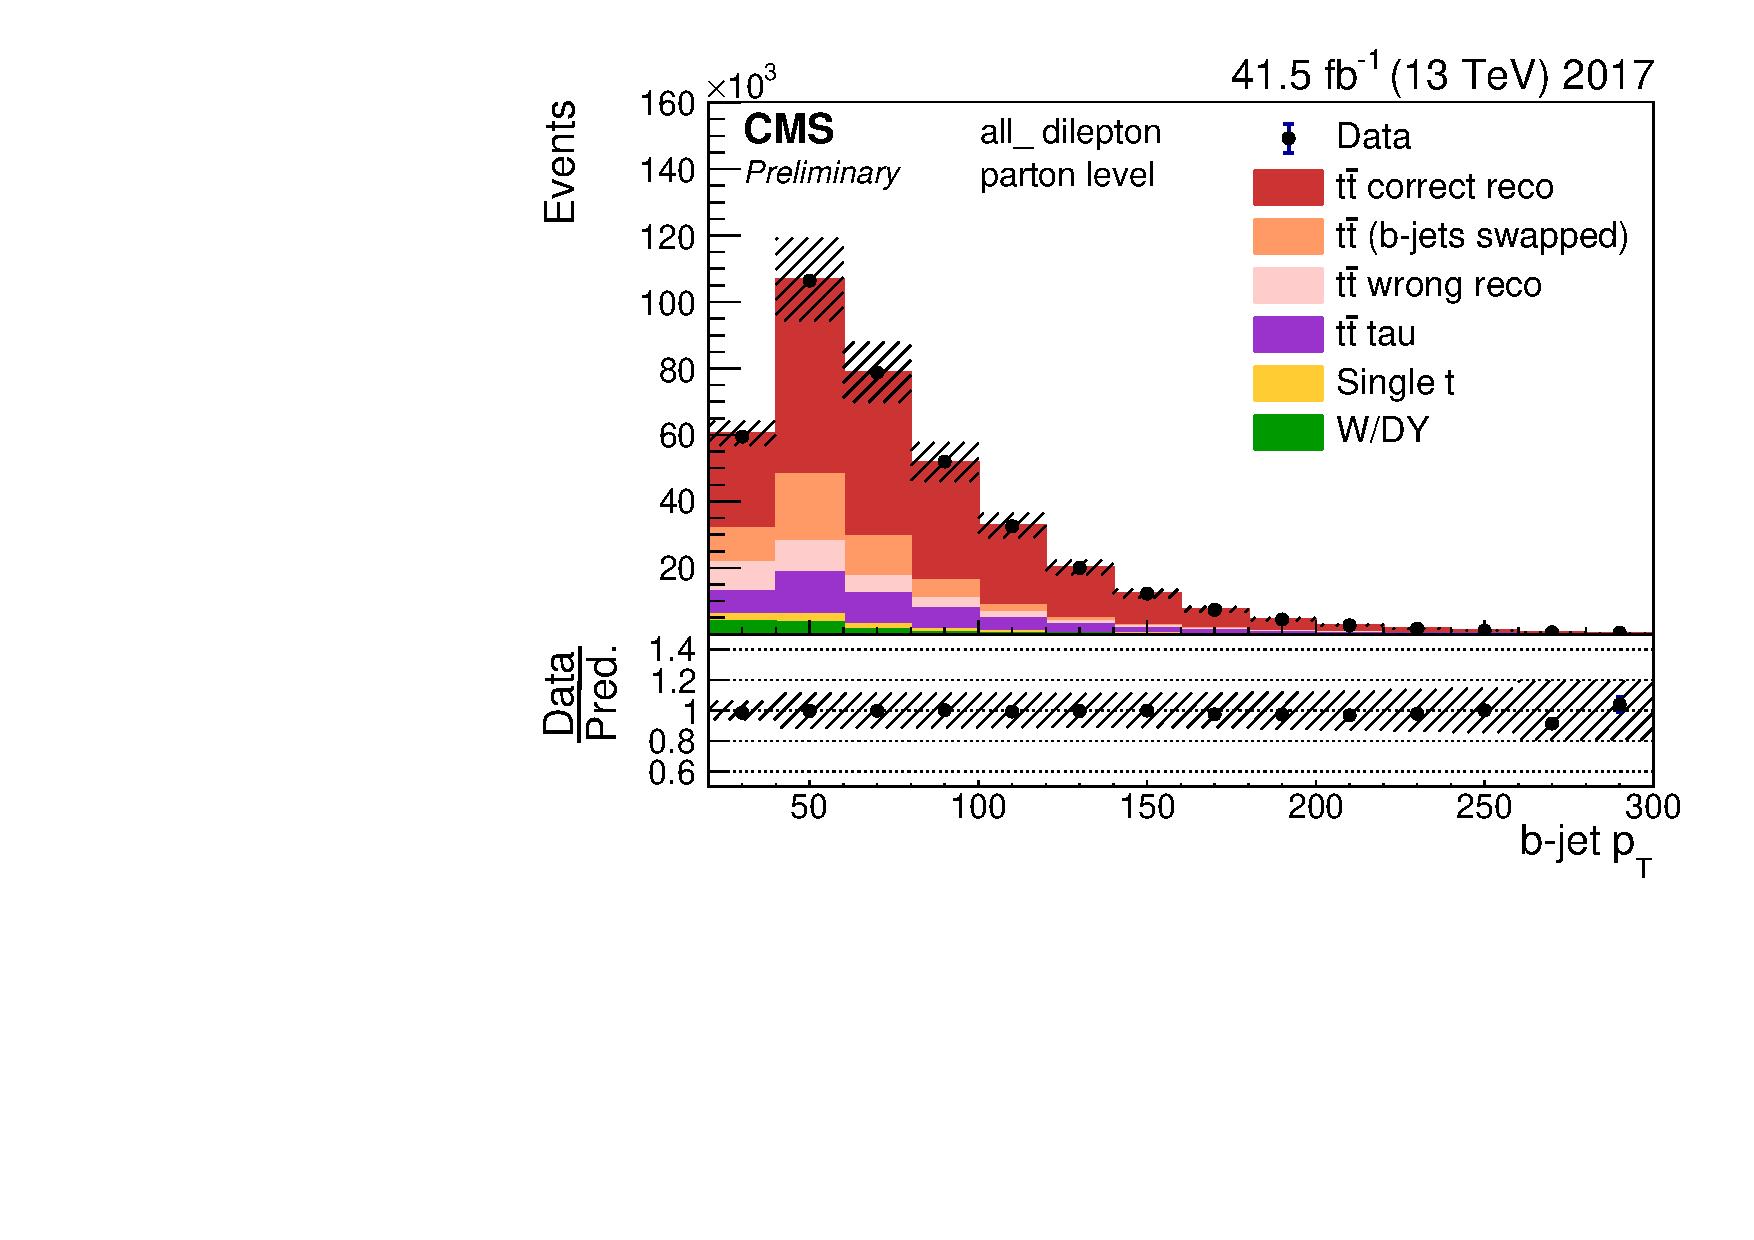
\includegraphics[width=.44\linewidth]{figs/bjpt_17.pdf}
%     \caption{2017 Data/MC agreement after neutrino/top reconstruction}
%     \label{fig:dmcpost_17}
% \end{figure}

\begin{figure}[h]
    \centering
    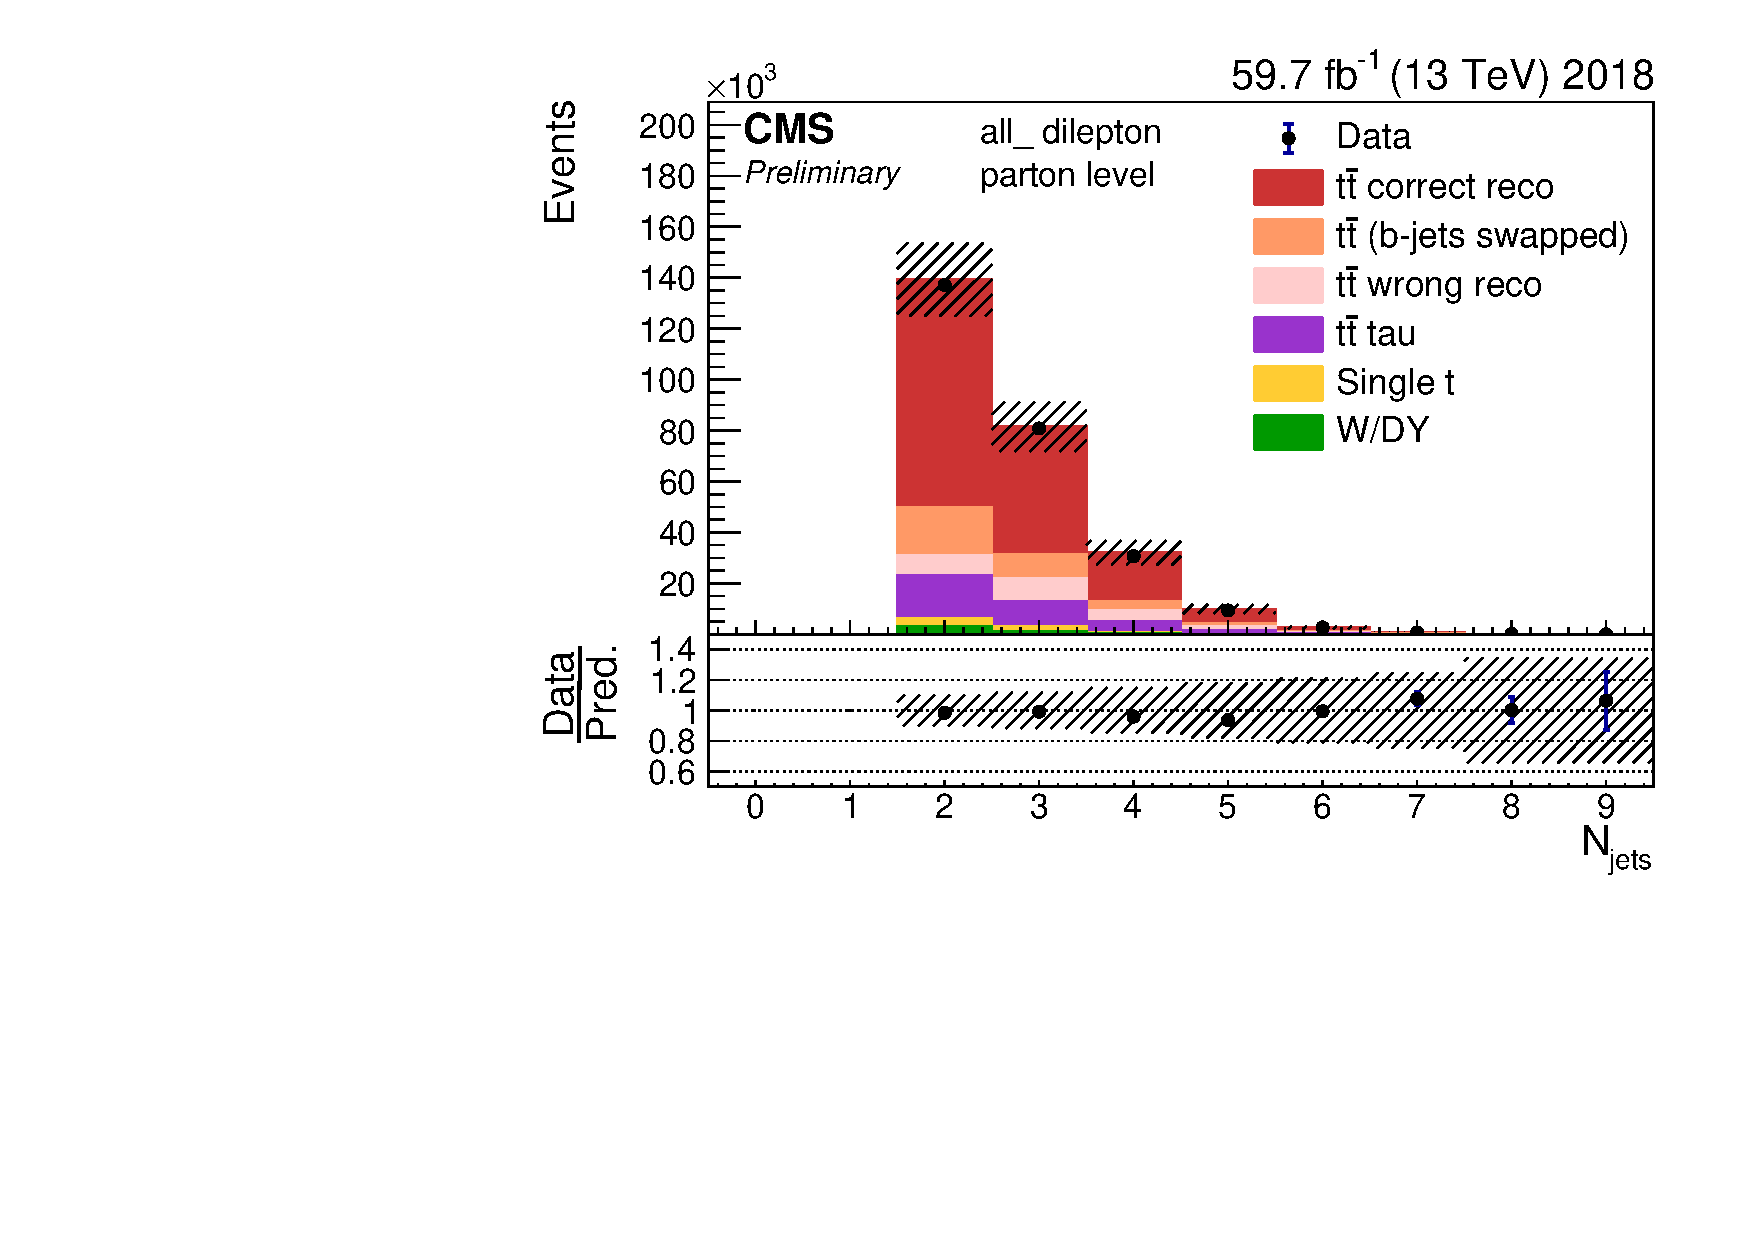
\includegraphics[width=.44\linewidth]{control/18_all_Njets.pdf}
    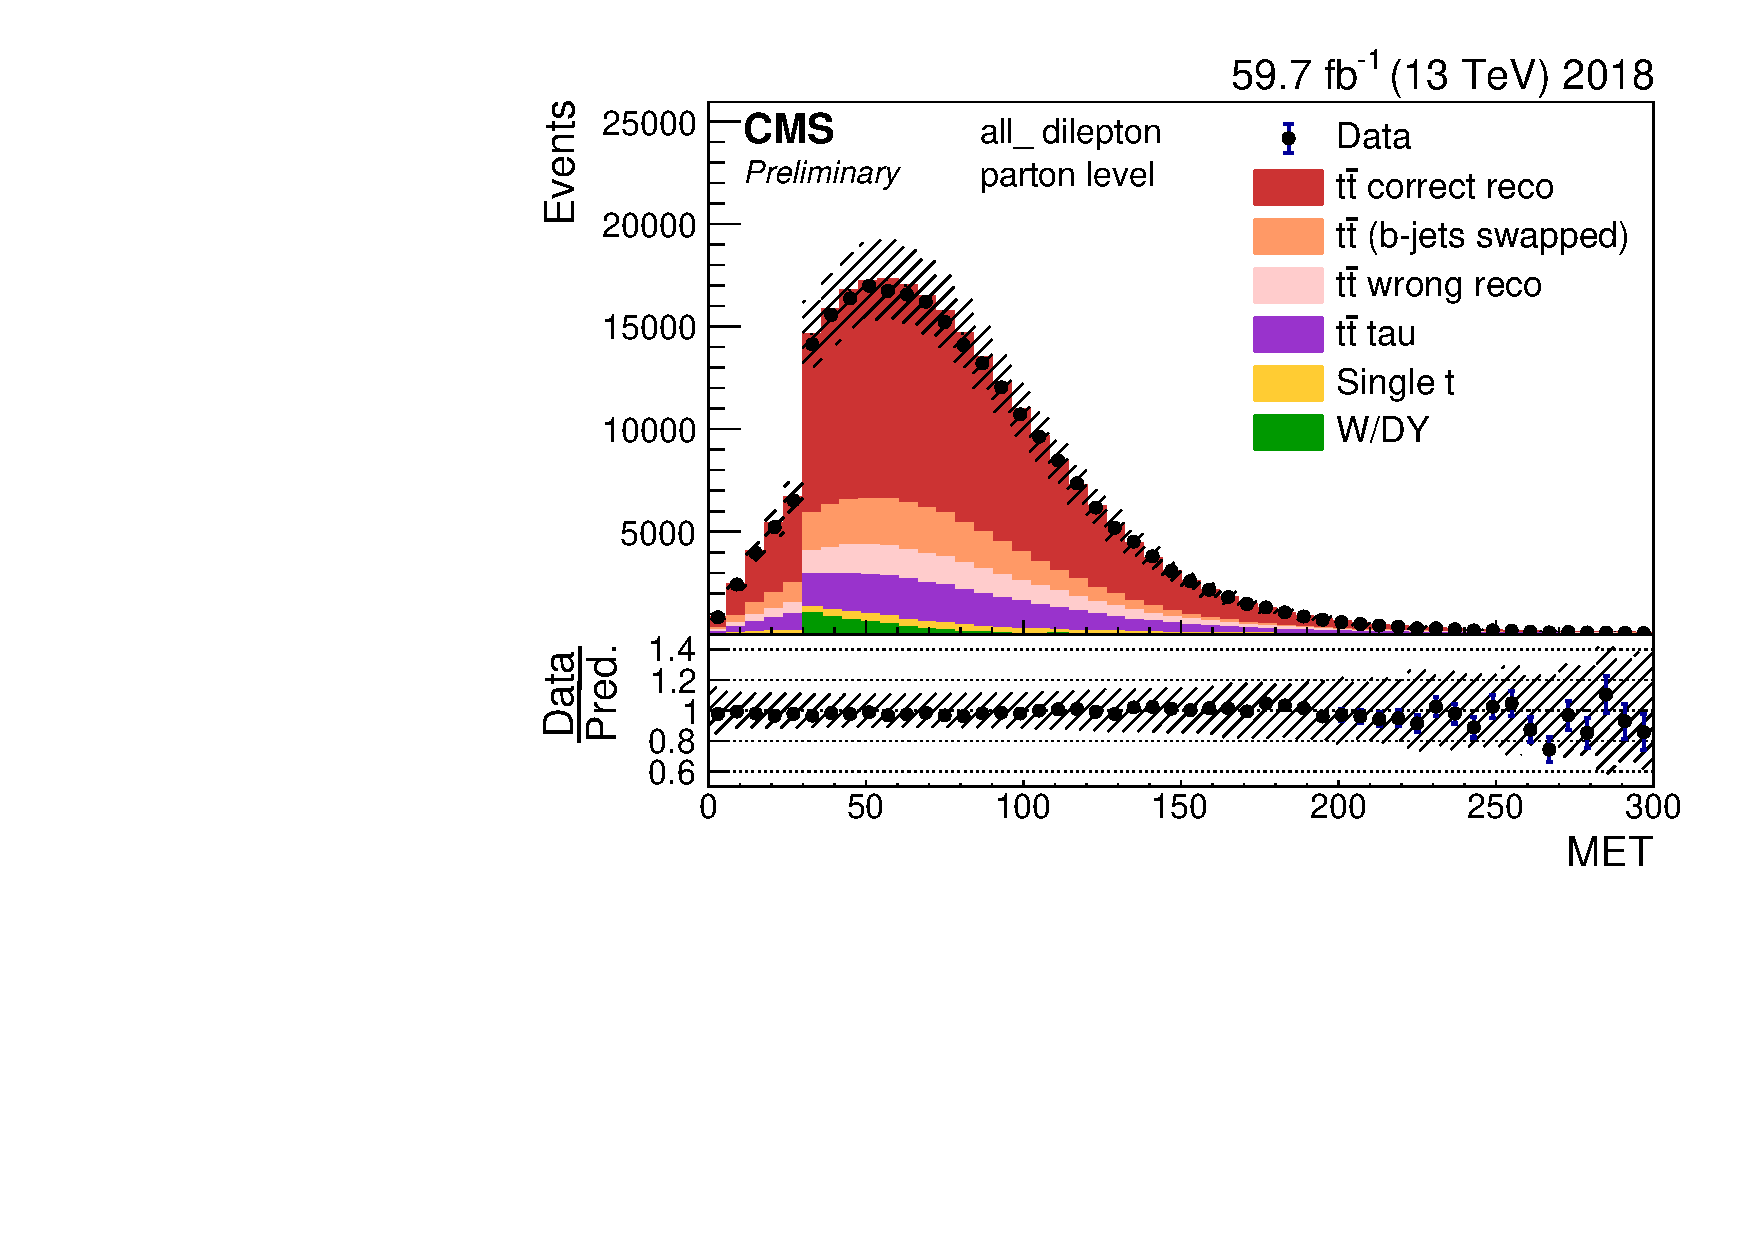
\includegraphics[width=.44\linewidth]{control/18_all_MET.pdf}
    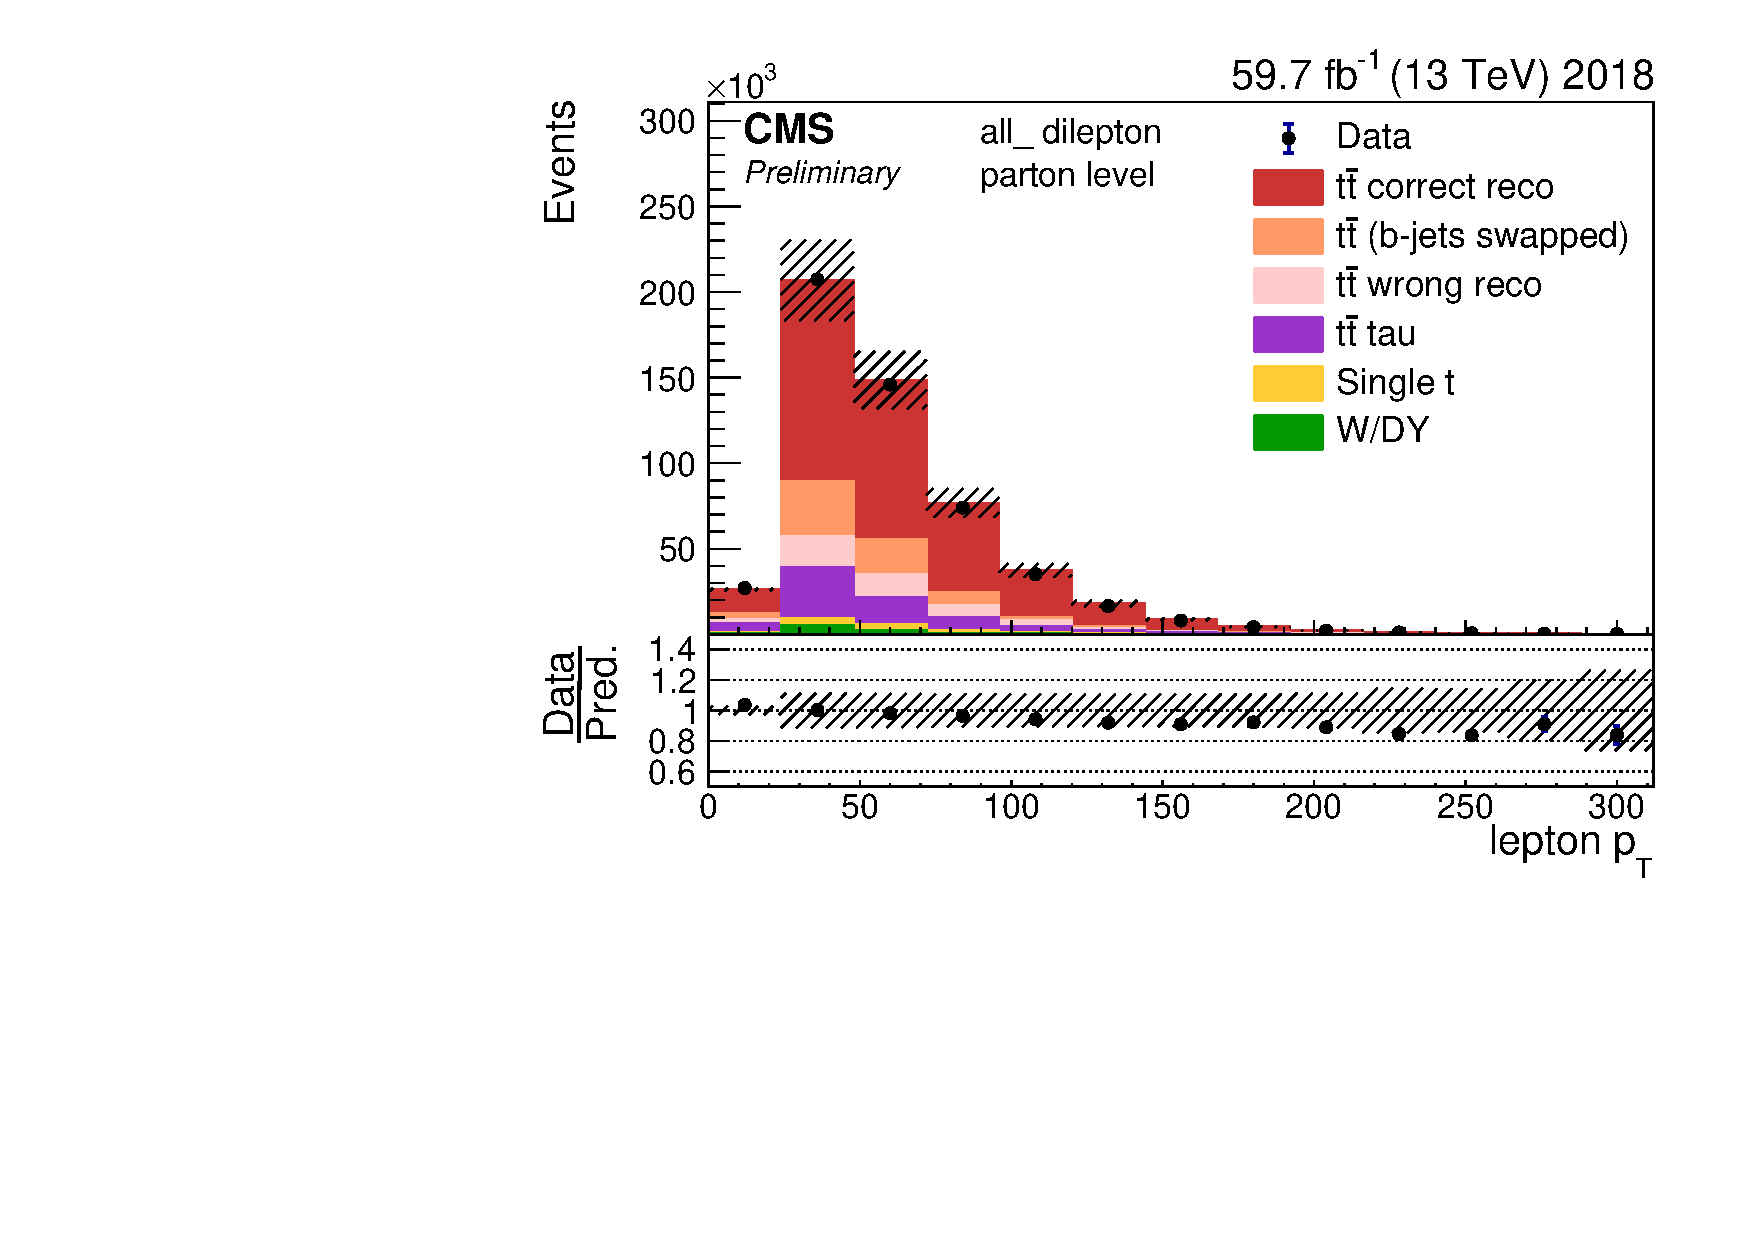
\includegraphics[width=.44\linewidth]{control/18_all_lep_pt.pdf}
    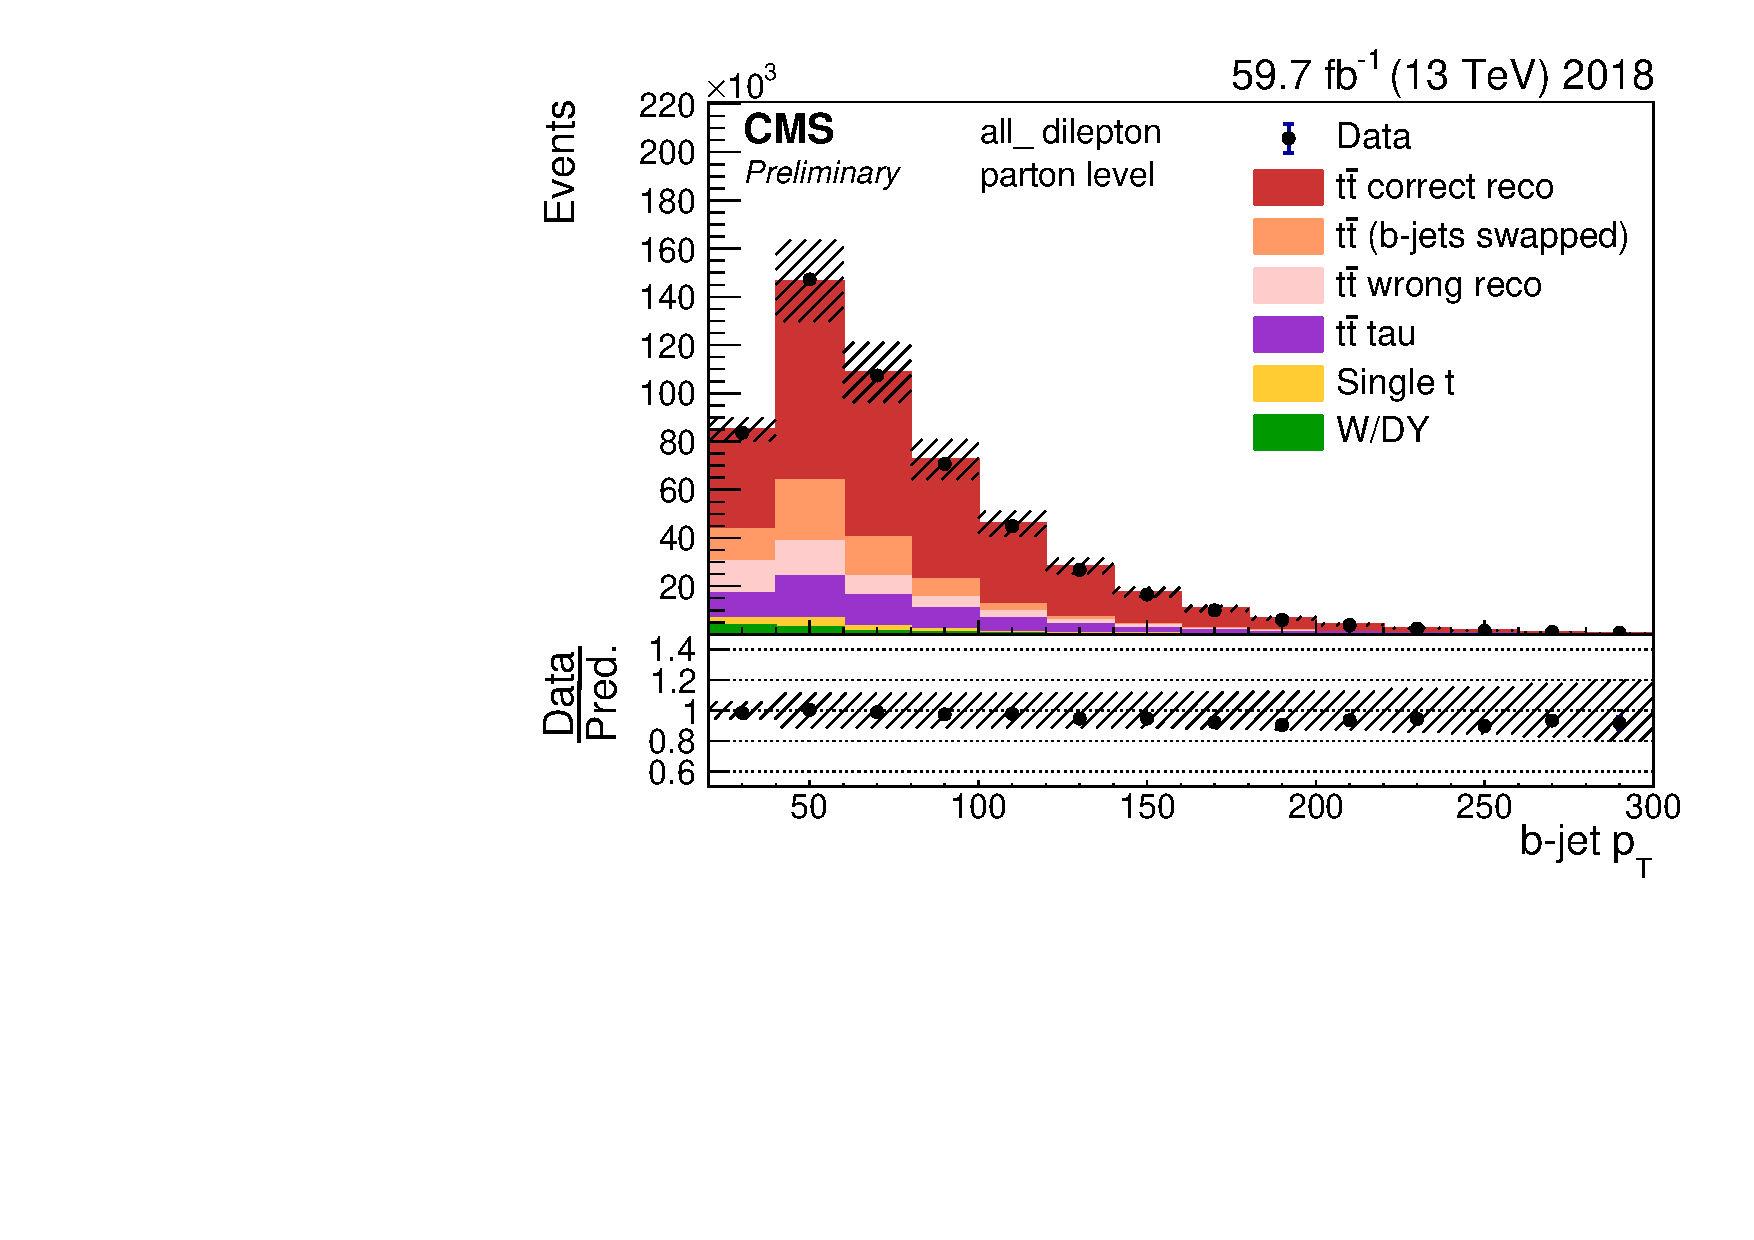
\includegraphics[width=.44\linewidth]{control/18_all_bj_Pt.pdf}
    \caption{2018 Data to MC comparison. }
    \label{fig:dmcpost_18}
\end{figure}

% \begin{figure}[h]
%     \centering
%     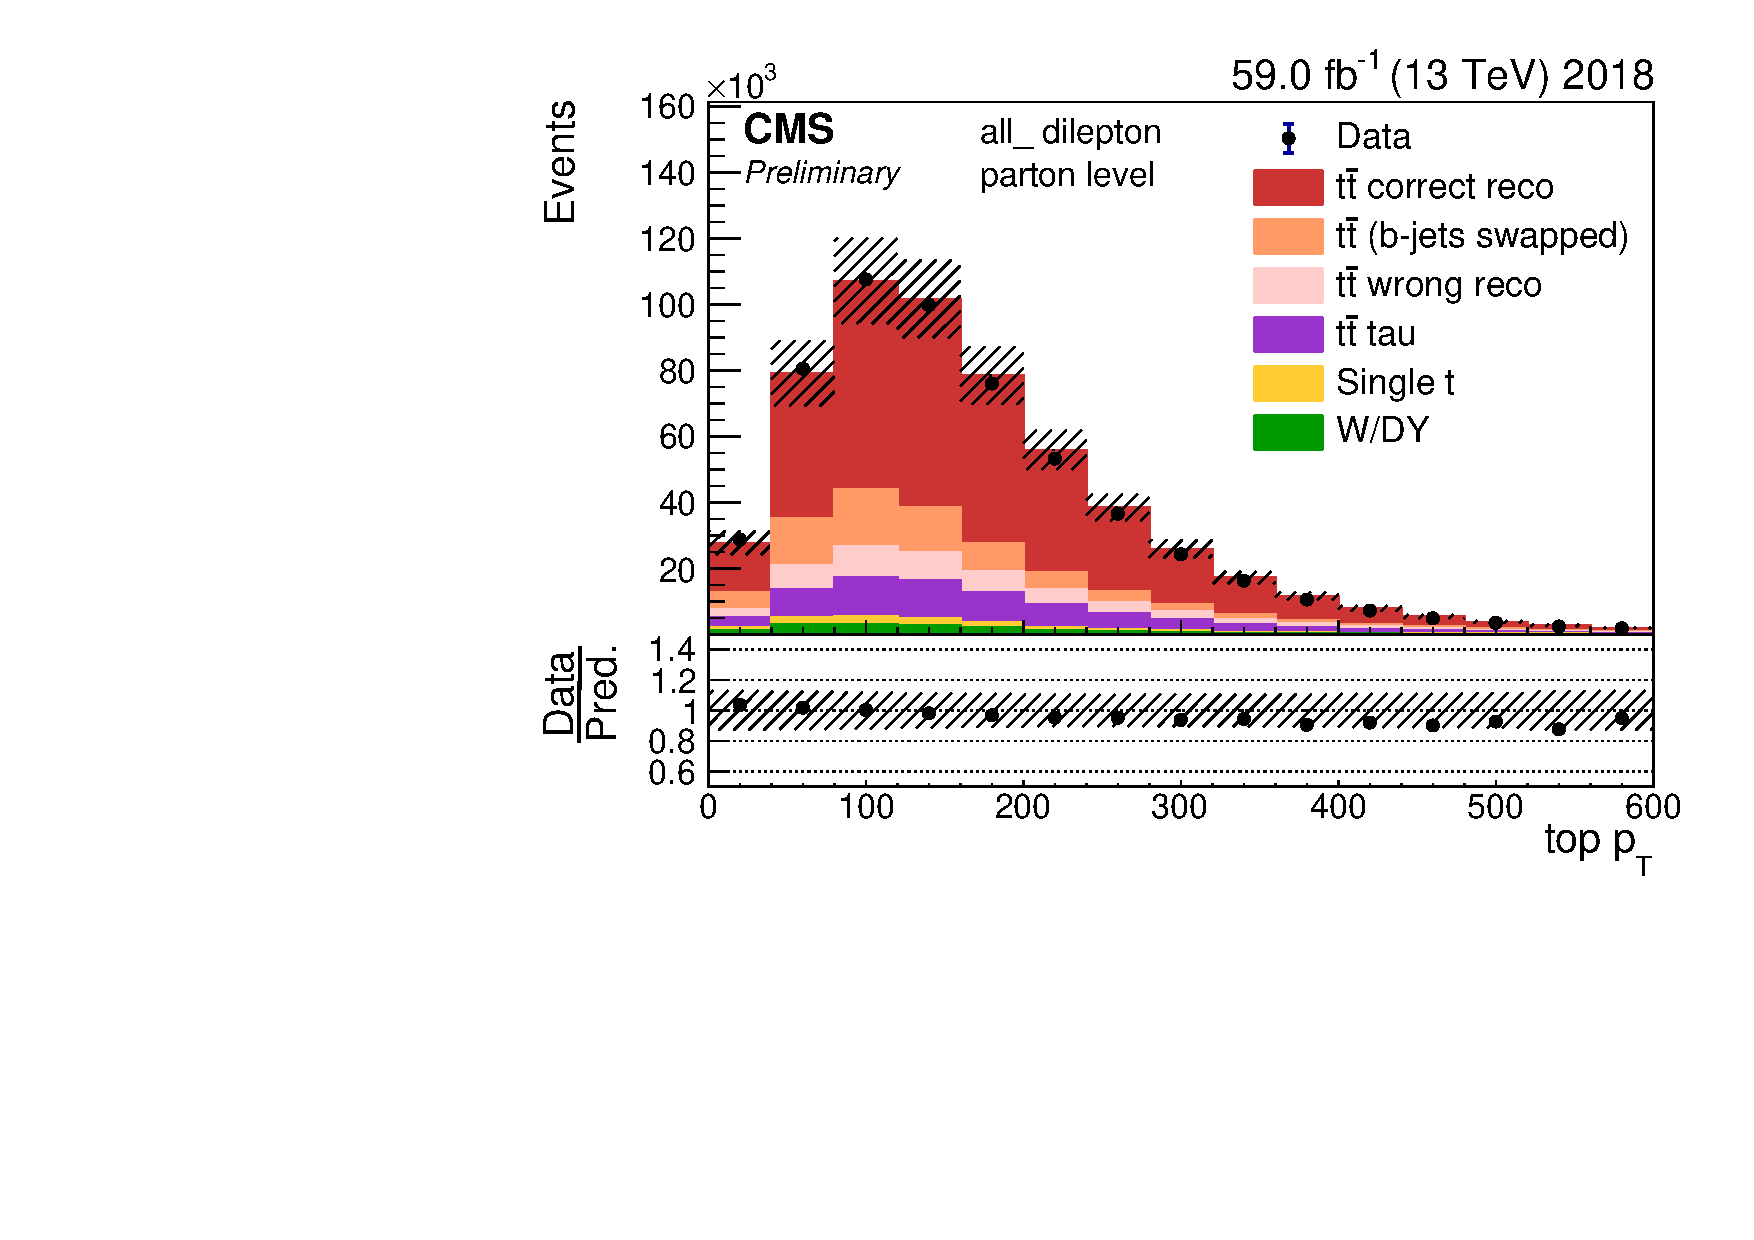
\includegraphics[width=.44\linewidth]{figs/toppt_18.pdf}
%     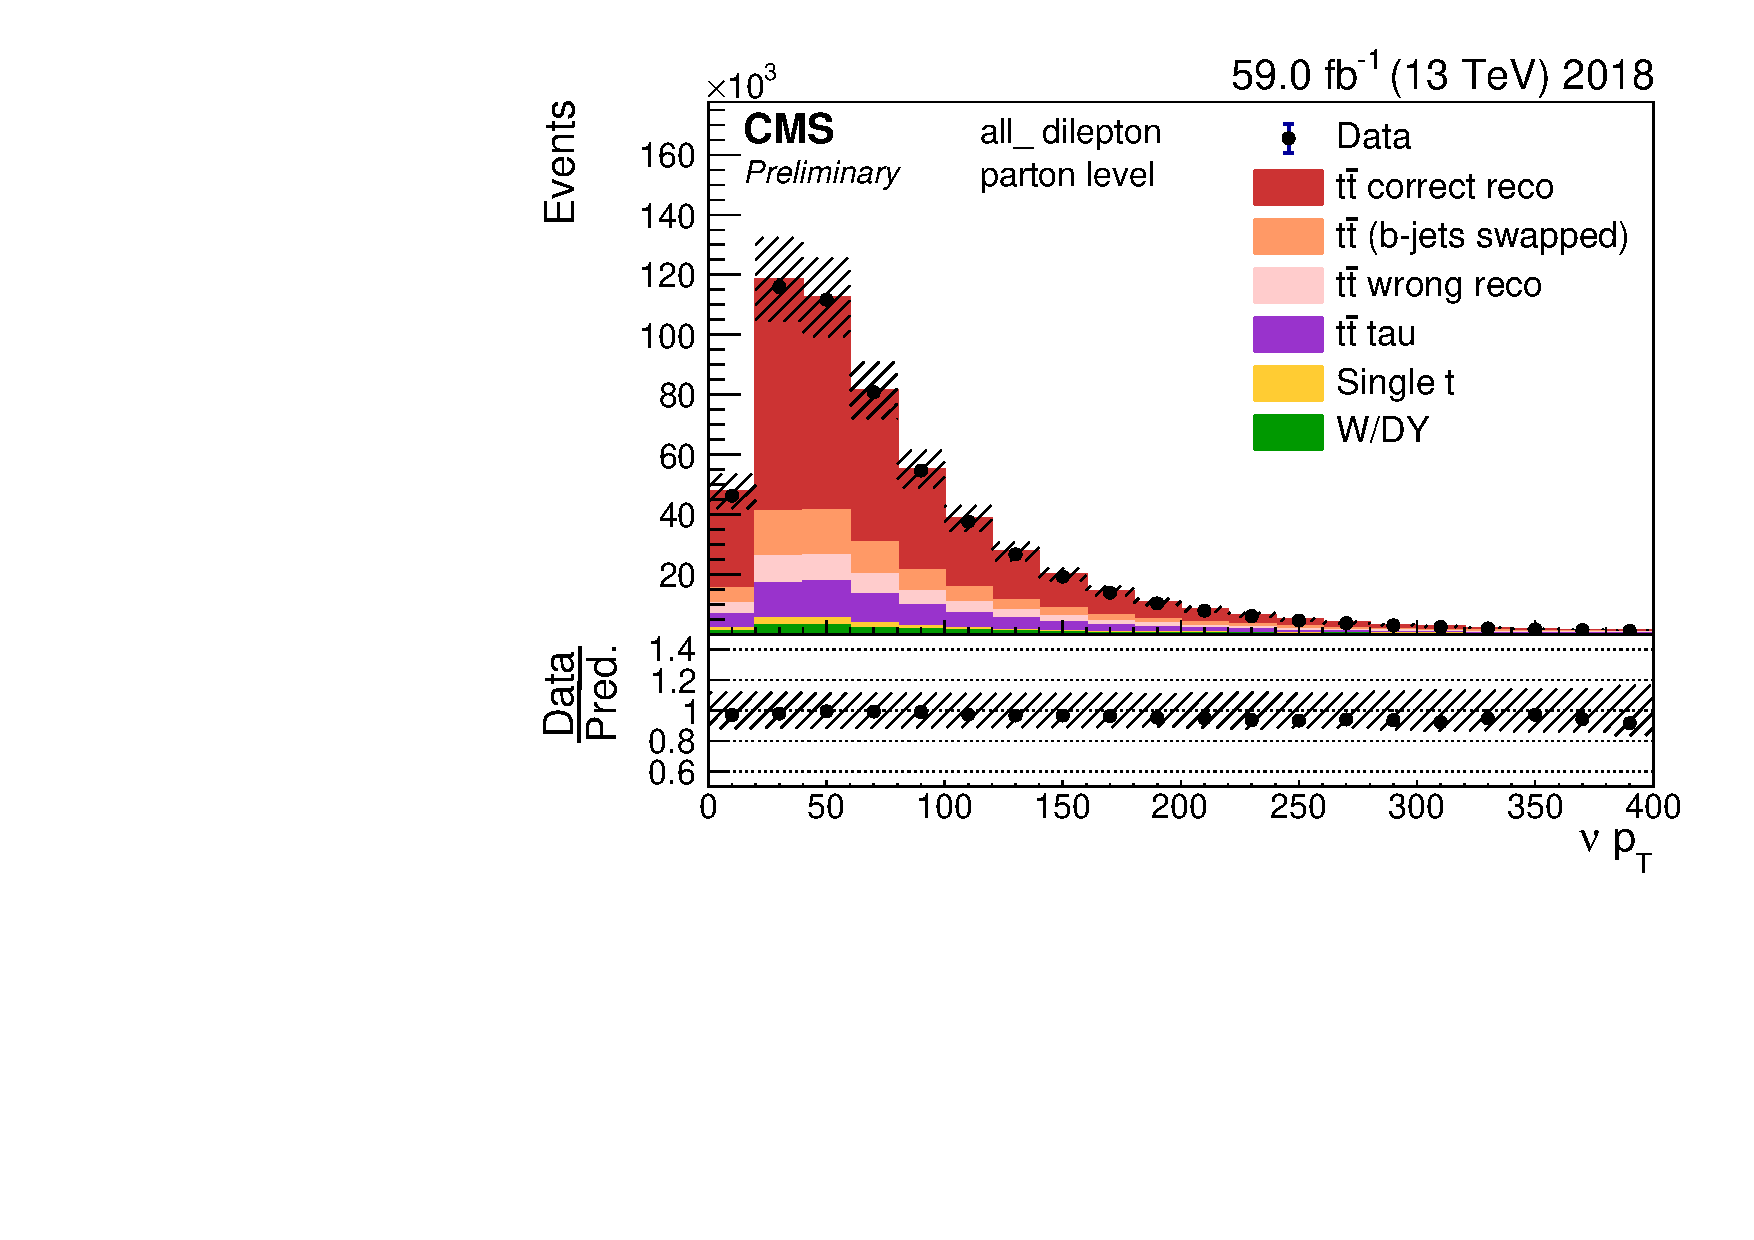
\includegraphics[width=.44\linewidth]{figs/nupt_18.pdf}
%     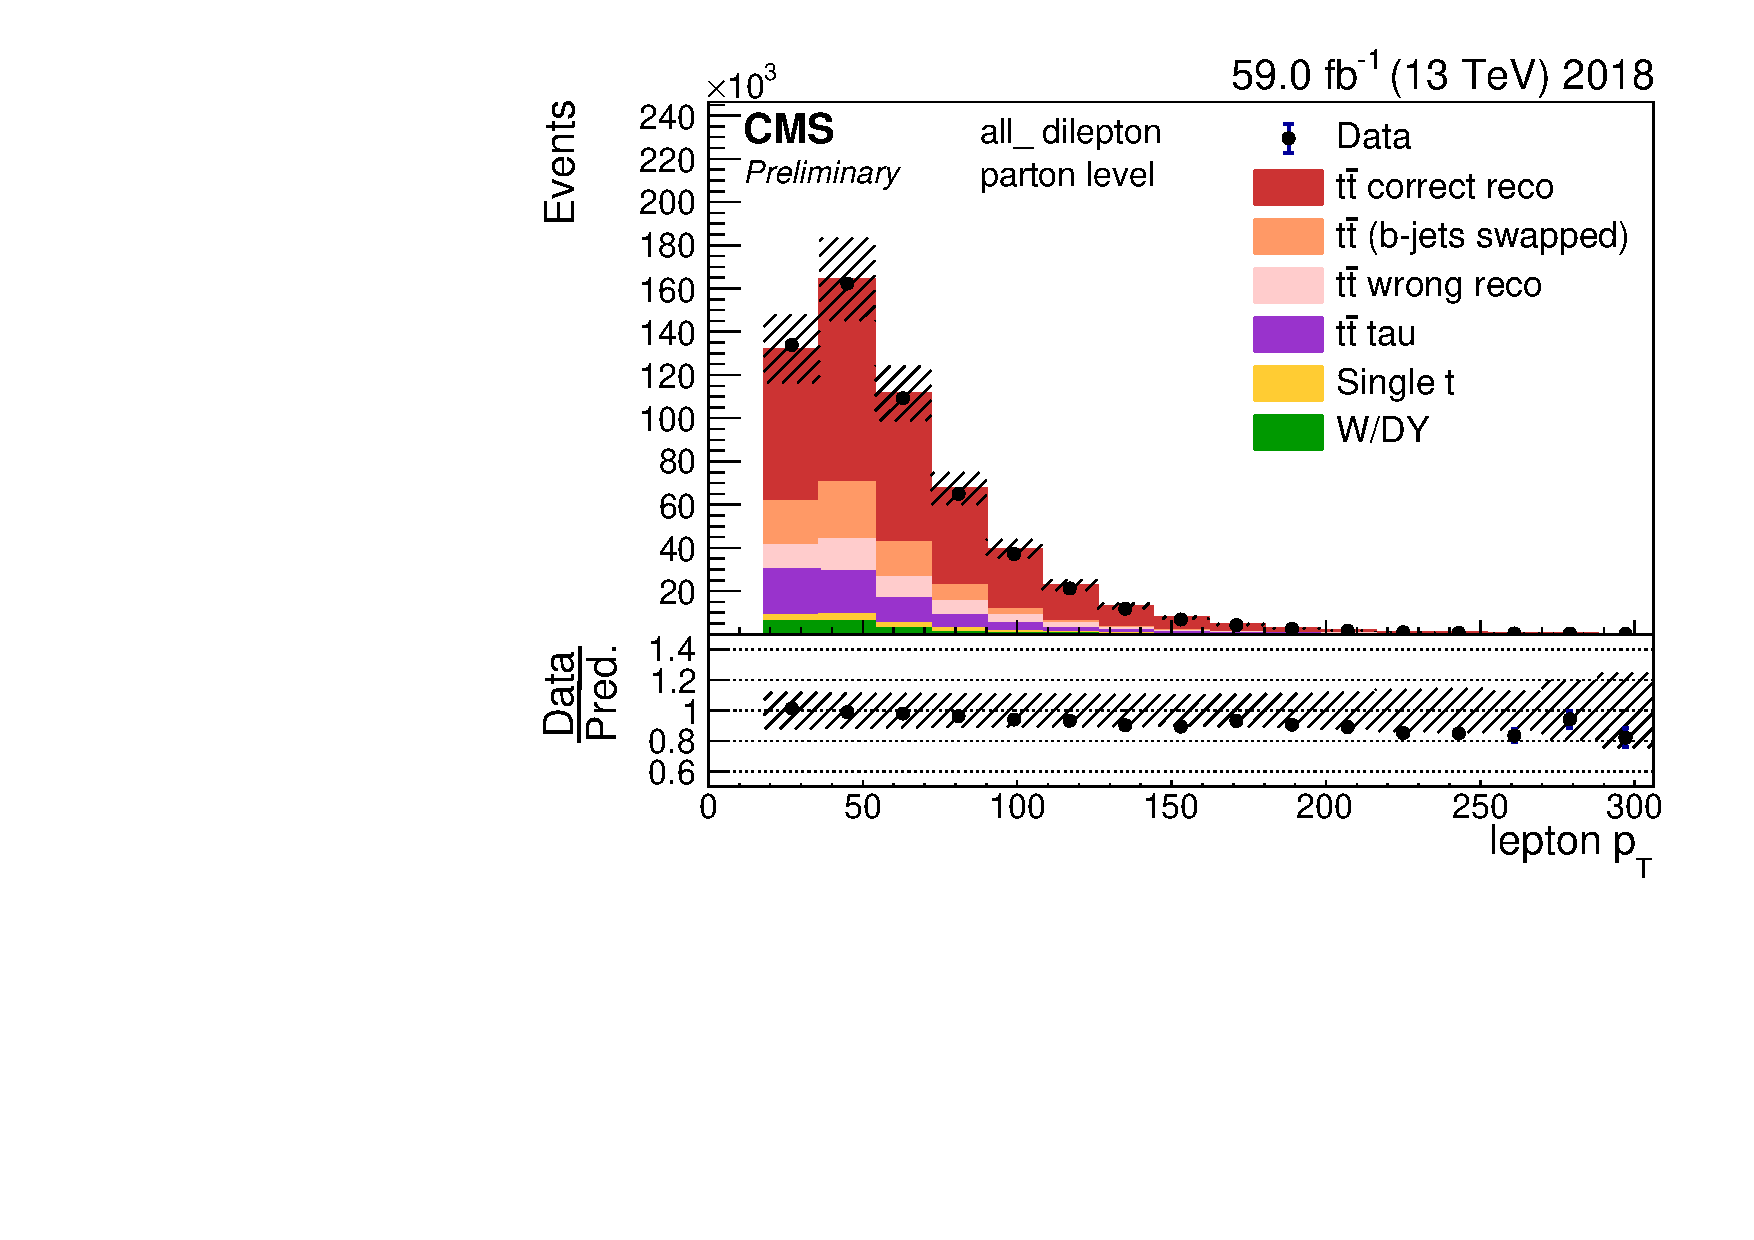
\includegraphics[width=.44\linewidth]{figs/leppt_18.pdf}
%     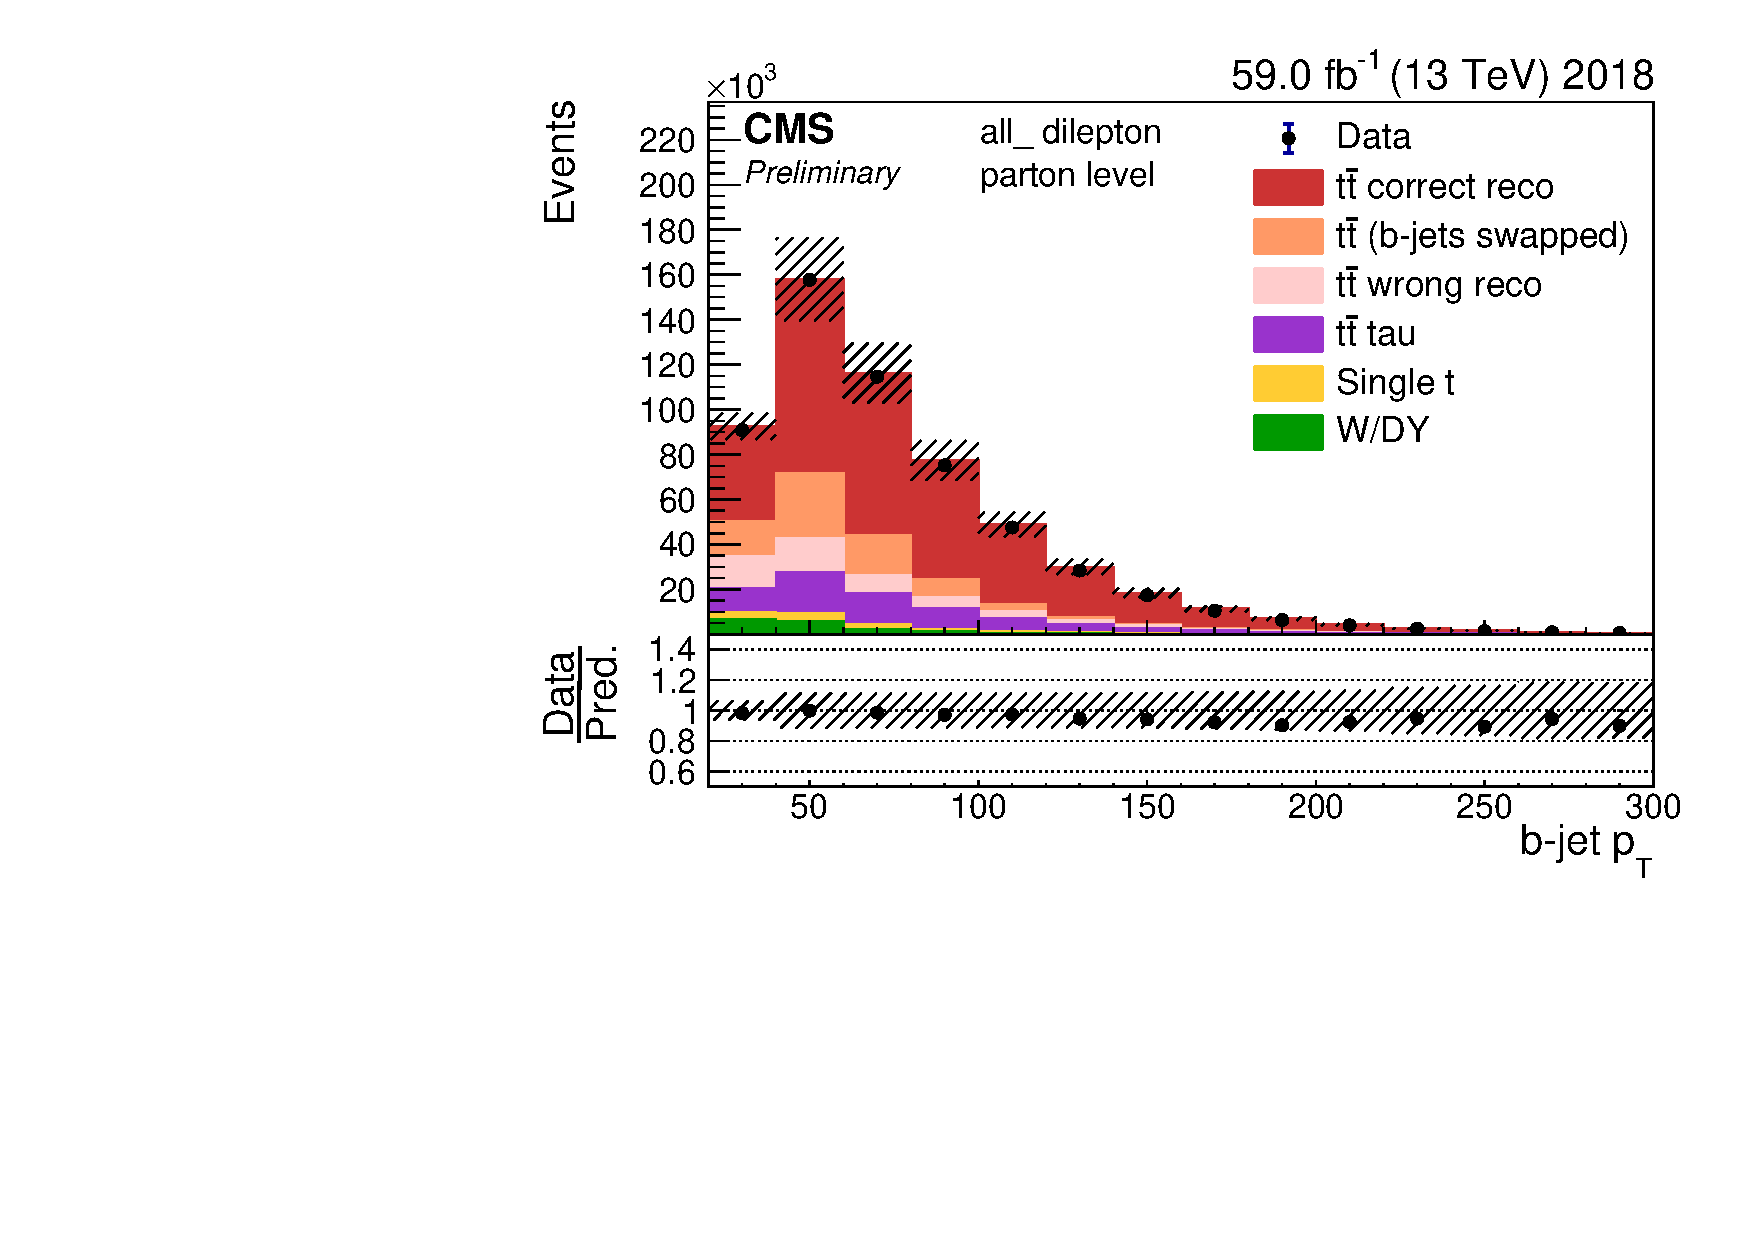
\includegraphics[width=.44\linewidth]{figs/bjpt_18.pdf}
%     \caption{2018 Data/MC agreement after neutrino/top reconstruction}
%     \label{fig:dmcpost_18}
% \end{figure}


\clearpage
\section{Measurement Strategy and Statistical Methods}
\label{S:stats}

%The first order electroweak corrections, included as interference terms, introduce a correction factor to the \ttbar differential cross section. This correction factor, $R _\mathrm{EW}$, is the ratio of the yield including LO Electroweak corrections to the LO QCD-based yield. It can also be expressed in terms of the marginal effect of electroweak corrections as $R _\mathrm{EW} = 1 + \delta _\mathrm{EW}$.

\subsection{Definitions involving EW corrections}
\label{SS:kfactor}

The standard jargon of perturbation theory can sometimes be confusing, when applied to the EW corrections, since perturbative expansions are done in orders of two separate coupling constants, $\alpha_s$ and $\alpha$. To clarify, we will utilize  notation similar to \cite{Czakon:2017NLOEW}, where a generic observable $\Sigma ^{t\bar{t}}$ is expanded in a series as

\begin{equation}
    \Sigma^{t\bar{t}}(\alpha_s,\alpha)=\sum_{m+n\geq 2} \alpha_s^m \alpha^n \Sigma _{m,n}
\end{equation}

In practice, contributions due to terms with $m<2$ or $n>2$ are small, and as such often neglected in the calculation of the differential cross sections. In this analysis the following contributions are of interest:

\begin{eqnarray}
    \Sigma_\mathrm{LO\; QCD} &=& \alpha_s ^2 \Sigma_{2,0}\\
    \Sigma_\mathrm{NLO\; QCD} &=& \alpha_s ^3 \Sigma_{3,0}\\
    \Sigma_\mathrm{NLO\; EW} &=& \alpha_s ^2 \alpha \Sigma_{2,1}\\
    \Sigma_\mathrm{extra\; EW} &=& \alpha_s ^3 \alpha \Sigma_{3,1}
\end{eqnarray}

In using the Hathor package to compute the differential cross section, as a function of \yt, we include the terms

\begin{equation}
    \Sigma_\textsc{HATHOR}(\yt) = \Sigma_\mathrm{LO\; QCD} + \Sigma_\mathrm{NLO\; EW}(\yt).
\end{equation}
The EW corrections K-factor can be defined at the LO QCD level:

\begin{equation}
    K^{\mathrm{NLO}}_\mathrm{EW} = \frac{ \Sigma_\mathrm{LO\; QCD} + \Sigma_\mathrm{NLO\; EW}}{\Sigma_\mathrm{LO\; QCD}}
\end{equation}

Meanwhile, the Powheg+Pythia samples include terms
\begin{equation}
    \Sigma_\textsc{POWHEG} = \left( \Sigma_\mathrm{LO\; QCD} + \Sigma_\mathrm{NLO\; QCD} \right)_{+\mathrm{PS}},
\end{equation}
Where the subscript ${+\mathrm{PS}}$ indicates that parton shower effects have been included as well. Potential variation of these parton shower effects should be covered by the standard procedure of evaluating such uncertainties. 
%While it would be nice to have a sample including EW terms with PS effects, these effects should be smaller than the fairly large uncertainty we will soon introduce on our EW corrections, so we won't devote much further discussion to them.

Since $\alpha \ll \alpha_s $, it often makes some sense to 
%choose some $N$ and 
work at fixed order $m\leq N$, $n\leq 1$, rather than at  $m+n\leq N$ (as mentioned in \cite{pagani2016photon}). Thus,  the EW corrections to the NLO QCD calculations are frequently included using the K-factor, defined at the LO QCD level:
\begin{equation}
    \Sigma_\mathrm{NLO\; QCD\times EW} \equiv K^{\mathrm{NLO}}_\mathrm{EW}\times \left( \Sigma_\mathrm{LO\; QCD} + \Sigma_\mathrm{NLO\; QCD} \right) 
    \label{eq:multiplicative1}
\end{equation}

We will refer to this as the ''multiplicative approximation", which is similar to the ``multiplicative approach" referenced in \cite{Czakon:2017NLOEW}, aside from the missing NNLO QCD terms, which are  covered by the uncertainty due to scale variations. This is the best approximation for EW corrections available to us, because in many kinematic regimes these corrections factorize from their QCD counterparts. Thus, this approach allows us to approximate the terms in $\Sigma_\mathrm{extra\; EW} $ in addition to those directly generated in HATHOR. Specific to this analysis are the dependence on \yt and the use of Powheg, so we can write out our formula for observables more explicitly as 

\begin{equation}
    \Sigma_\mathrm{NLO\; QCD\times EW}^{\yt} \equiv K^{\mathrm{NLO}}_\mathrm{EW} (\yt)\times \Sigma_\textsc{POWHEG}
    \label{eq:multiplicative2}
\end{equation}

In order to estimate the uncertainty on this approach to including EW corrections, we investigate also the more naive additive approach,
\begin{equation}
\Sigma_\mathrm{NLO\; QCD+ EW}^{\yt} \equiv \left(K^{\mathrm{NLO}}_\mathrm{EW}\times \Sigma_\mathrm{LO\; QCD}\right) + \Sigma_\mathrm{NLO\; QCD},
\end{equation}

which neglects  the term  $\Sigma_\mathrm{extra\; EW} $ entirely. We take the difference between the two approaches as an uncertainty of the method:
\begin{eqnarray}
\mathrm{EW\;unc.} &=& \Sigma_\mathrm{NLO\; QCD\times EW}^{\yt} - \Sigma_\mathrm{NLO\; QCD+ EW}^{\yt}\label{eq:uncline1} \\ 
&=& \left(\Sigma_\textsc{POWHEG} - \Sigma_\mathrm{LO\; QCD} \right)(K^{\mathrm{NLO}}_\mathrm{EW}(\yt) - 1 )\label{eq:uncline2} \\
 &\equiv& (\Sigma_\textsc{POWHEG}\times \delta_\mathrm{QCD}) \times (\delta_\mathrm{EW}),
\label{eq:uncline3}
\end{eqnarray}
where we have introduced the shorthand 
\begin{equation}
\delta_\mathrm{QCD}=\frac{\Sigma_\textsc{POWHEG} - \Sigma_\mathrm{LO\; QCD} }{\Sigma_\textsc{POWHEG}}, \;\;\;\; \delta_\mathrm{EW} =(K^{\mathrm{NLO}}_\mathrm{EW}(\yt) - 1 ),
\end{equation}
to illustrate that this uncertainty is effectively a cross term which arises from the difference in additive and multiplicative approaches. Note that $\delta_\mathrm{EW}$ represents the usual marginal effect in terms of which EW corrections are often understood.

The implementation of this uncertainty is detailed in Section \ref{SS:statmeth}. Though this is almost certainly an overestimation, it is difficult to ascribe a more accurate uncertainty without actually computing the missing terms in $\Sigma_\mathrm{extra\; EW} $. 
%This may be possible with the Sherpa generator, but varying the top Yukawa coupling is often outside of the intended use of Monte Carlo generators, and may require some coordination with the Sherpa authors.

\subsection{Implementation of EW corrections}

Events are reweighted with the additional weight factor of $w_\mathrm{EW}(\yt)$ to account for the effects of 1-loop EW corrections which enter at $\mathcal{O}(\alpha_\mathrm{S}^2\alpha)$. We use the HATHOR package to generate the weights $w_\mathrm{EW}$ as a 2-dimensional function of $M_{\ttb}$ and $\Delta y $. These weight correction is generated and applied to partons at generator level in our \ttbar MC samples for a set of discrete values $\yt=0,1,...,5$. Reconstruction is carried out and the resulting double-differential distribution of events in $M_{\mathrm{bl}}$ and $\Delta y_{\mathrm{bl}}$ is stored for each $\yt$ value.

\begin{figure}
    \centering
    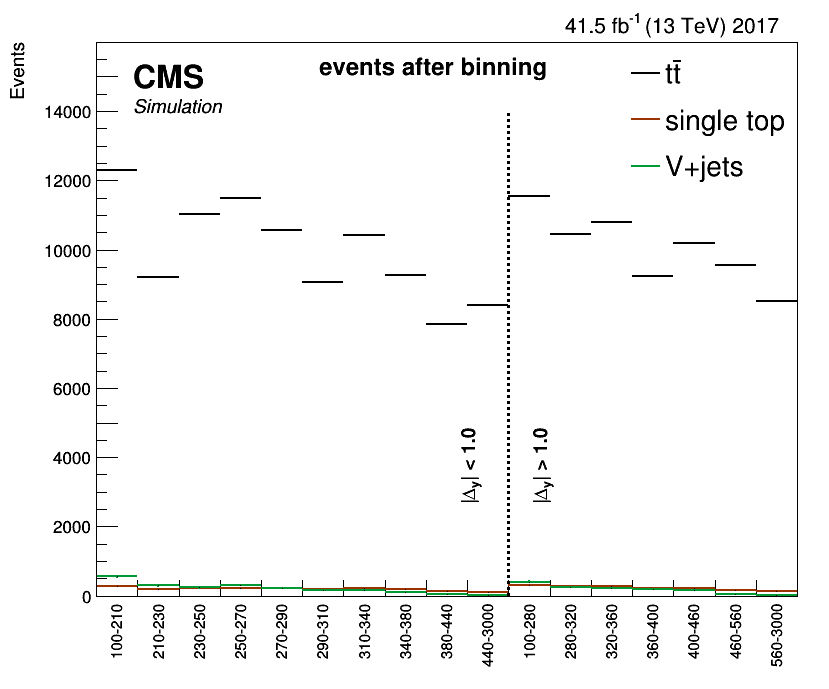
\includegraphics[width=.7\linewidth]{figs/ttbinned.png}
    \caption{\ttbar MC  events after reconstruction and binning, 2017. The dashed line divides the two \absDybl bins, while the horizontal axis shows the bins' \Mbl ranges}
    \label{fig:ttbinned}
\end{figure}

After reconstruction, events are binned coarsely in $|\Delta y_{\mathrm{bl}}|$ and more finely in $M_{\mathrm{bl}}$. The binning is chosen such that no year will have fewer than 5,000 signal events in any given bin \ref{fig:ttbinned}. In each bin, the yield is examined as a function of $\yt$.  The effect is almost exactly quadratic as a consequence of the main diagrams involved (Figure \ref{fig:diagrams}), so we perform a quadratic fit to extrapolate the effect of the EW correction on a given bin as a continuous function of $\yt$ (figure \ref{fig:quad}). This correction for each bin can be applied as a rate parameter $R_\mathrm{EW}^\mathrm{bin}(\yt) = 1 +  \delta _\mathrm{EW}(\yt)$ affecting the expected bin content. 

\subsection{Statistical treatment in Combine}
\label{SS:statmeth}

Using this approach, we use the Combine statistics package to obtain the best  fit for the parameter of interest (POI), $\yt$. Combine maximizes a likelihood function $\mathcal{L}$, which is defined as a product over bins, 

\begin{equation}
    \mathcal{L} = \prod_{\mathrm{bin}\in (\Mbl,|\Delta y|_{bl}) } \mathcal{L}_\mathrm{bin}\;,
\end{equation}
where  the likelihood in each bin is a product of the Poisson probability for a statistical fluctuation and a penalty term for nuisance parameters, which deviate from their nominal/expected values:
% \begin{equation}
%     \mathcal{L}_\mathrm{bin} = \mathrm{Poisson}\Big[n^\mathrm{bin}_\mathrm{observed}  \Big\vert n^\mathrm{bin}_\mathrm{expected} (\mathrm{nuisances})\Big] \times \rho(\mathrm{nuisances}\vert\mathrm{expected})
% \end{equation}
% Filling in the details for this analysis, we have
\begin{equation}
    \mathcal{L}_\mathrm{bin} = \mathrm{Poisson}\Big[n^\mathrm{bin}_\mathrm{obs}  \Big\vert s^\mathrm{bin}(\{\theta_i \}) \times R_\mathrm{EW}^\mathrm{bin}(\yt, \phi) +b^\mathrm{bin}(\{\theta_i\}) \} \Big] \times p(\phi)\times \prod_i p(\theta_i).
\end{equation}

Here $n^\mathrm{bin}_\mathrm{obs}$ is the total observed bin count, with the expected bin count being the sum of  the predicted signal $s^\mathrm{bin}$ and background $b^\mathrm{bin}$. The number of expected signal events is modified by the additional rate $R_\mathrm{EW}$, which depends on the Yukawa coupling ratio $\yt$ and the special nuisance $\phi$, discussed further below.
%The parameter $\phi$ is separated  from the other parameters due to its special interaction with the EW corrections from which the measurement is derived.
Each of the other nuisance parameters, $\{\theta_i\}$, that affect the expected counts in each bin, is described by a gaussian probability distribution function of $p(\theta_i)$ that describes the likelihood of the deviation of $\theta_i$ from its expected value.  The correlations between nuisance parameters are discussed in Section~\ref{SS:corr}. 

We include an estimate of the uncertainty on the multiplicative application of EW corrections derived at order $\mathcal{O}(\alpha_\mathrm{S}^2\alpha)$, as discussed in Section \ref{SS:kfactor}. The full expression for the rate $R_\mathrm{EW}^\mathrm{bin}$, including this uncertainty term, is
\begin{equation}
    R_\mathrm{EW}^\mathrm{bin}(\yt, \phi) = (1+ \delta_\mathrm{EW}^\mathrm{bin}(\yt))\times(1+\delta_\mathrm{QCD}^\mathrm{bin}\delta_\mathrm{EW}^\mathrm{bin}(\yt))^\phi,
\end{equation}
where $\delta_\mathrm{QCD}^\mathrm{bin}\delta_\mathrm{EW}^\mathrm{bin}$ represents the cross term arising from the difference in multiplicative and additive approaches, based on Equations \ref{eq:uncline1}. The normally distributed nuisance parameter $\phi$ modulates this uncertainty. The definitions of Section \ref{SS:kfactor} are applied in terms of the expected bin yields $n^\mathrm{bin}$ after reconstruction:

\begin{eqnarray}
\delta_\mathrm{EW} =& (K^{\mathrm{NLO}}_\mathrm{EW}(\yt) - 1 ) \;\longrightarrow\;& \delta_\mathrm{EW}^\mathrm{bin}= \frac{n^{\mathrm{bin}}_\mathrm{\textsc{HATHOR}}-n^\mathrm{bin}_\mathrm{LO}}{n^\mathrm{bin}_\mathrm{LO}} \\
\delta_\mathrm{QCD} =& \frac{\Sigma_\textsc{POWHEG} - \Sigma_\mathrm{LO\; QCD} }{\Sigma_\textsc{POWHEG}} \;\longrightarrow\;& \delta_\mathrm{QCD}^\mathrm{bin}= \frac{n^{\mathrm{bin}}_\mathrm{\textsc{POWHEG}}-n^\mathrm{bin}_\mathrm{LO}}{n^\mathrm{bin}_\mathrm{POWHEG}} 
\end{eqnarray}

%where $\phi$ modulates the uncertainty on the EW corrections, obeying a normal distribution. 
We note that the uncertainty on the EW corrections is unique because it depends on the value of \yt, at which the EW corrections are evaluated. Thus, it is given its own term and nuisance parameter $\phi$ separate from other systematic uncertainties.

Our datacard construction and statistical methods follow the procedures described previously in \cite{ytnote}.

\begin{figure}
\centering
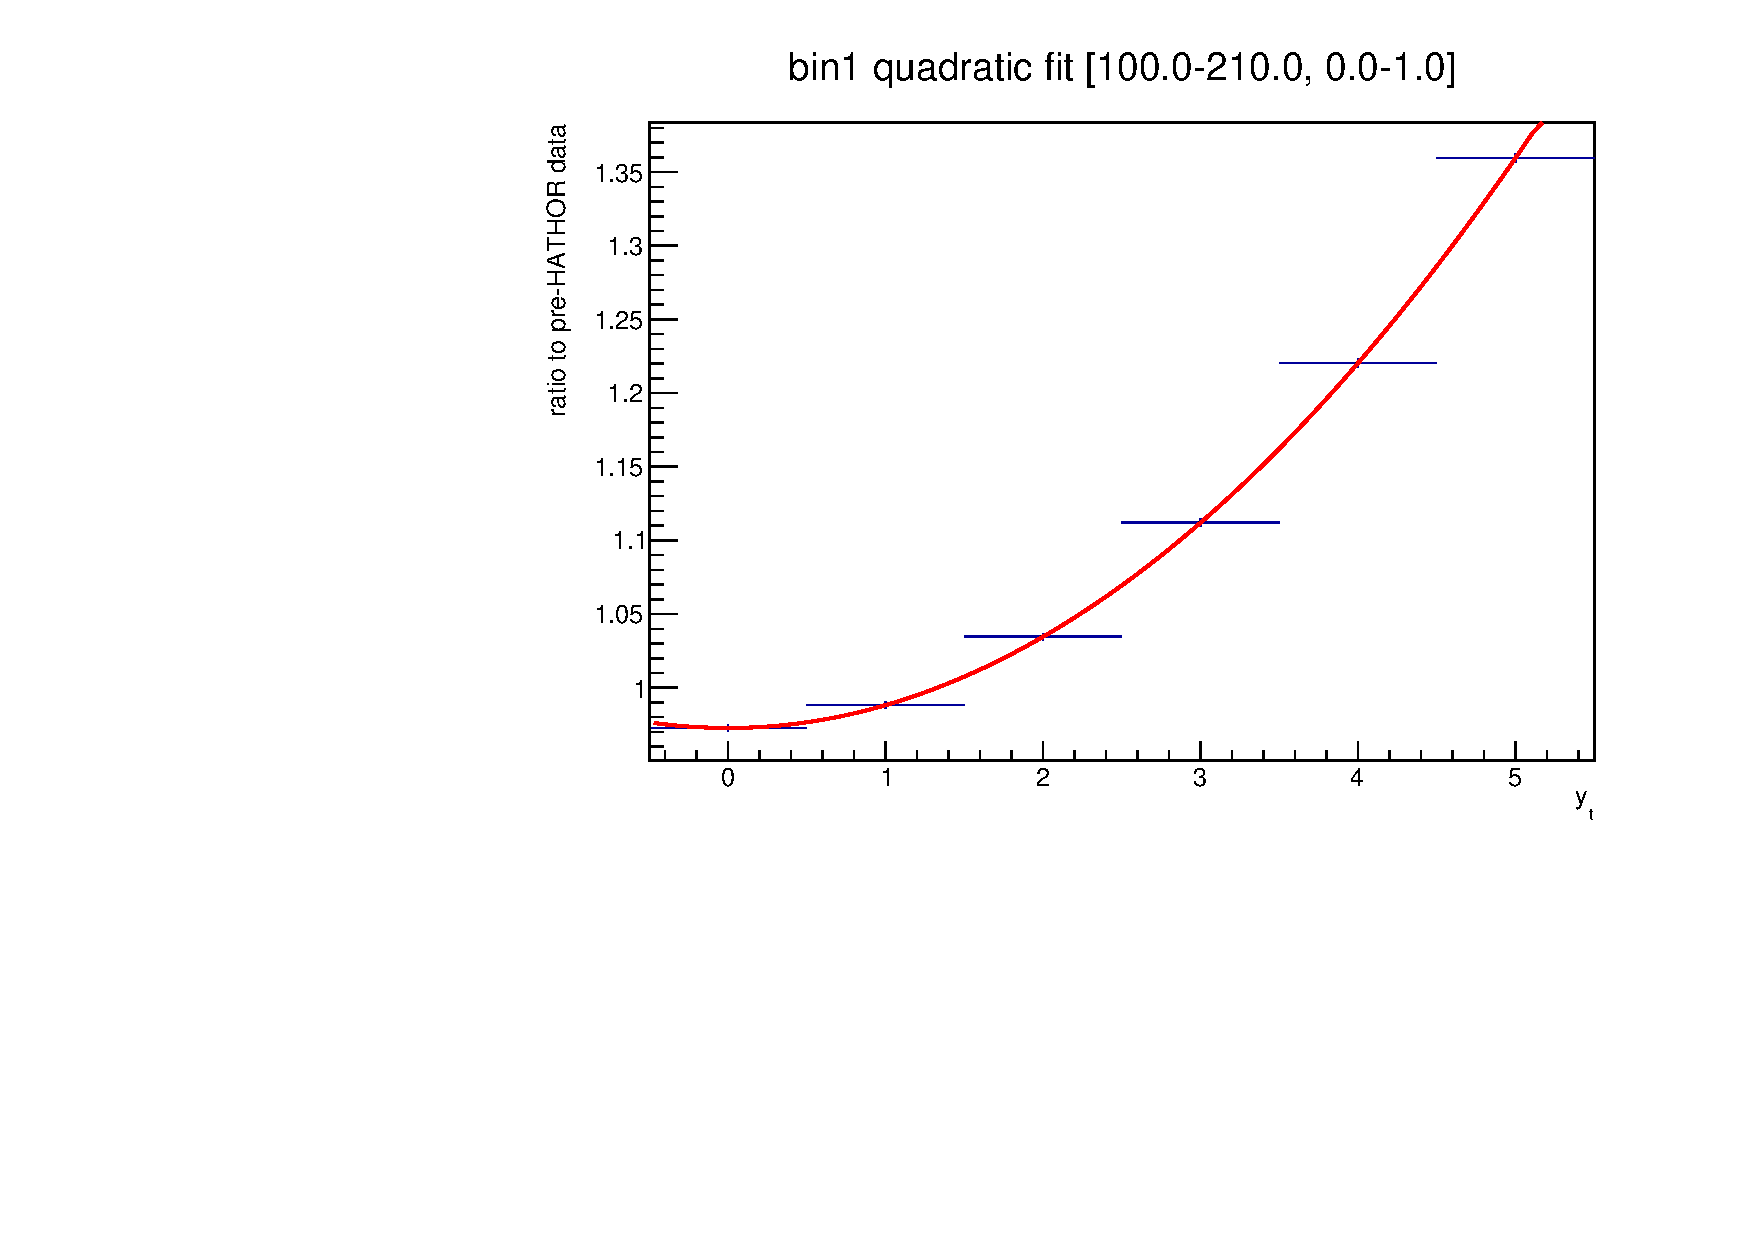
\includegraphics[width=.48\linewidth]{quadplots/2017bin1.pdf}
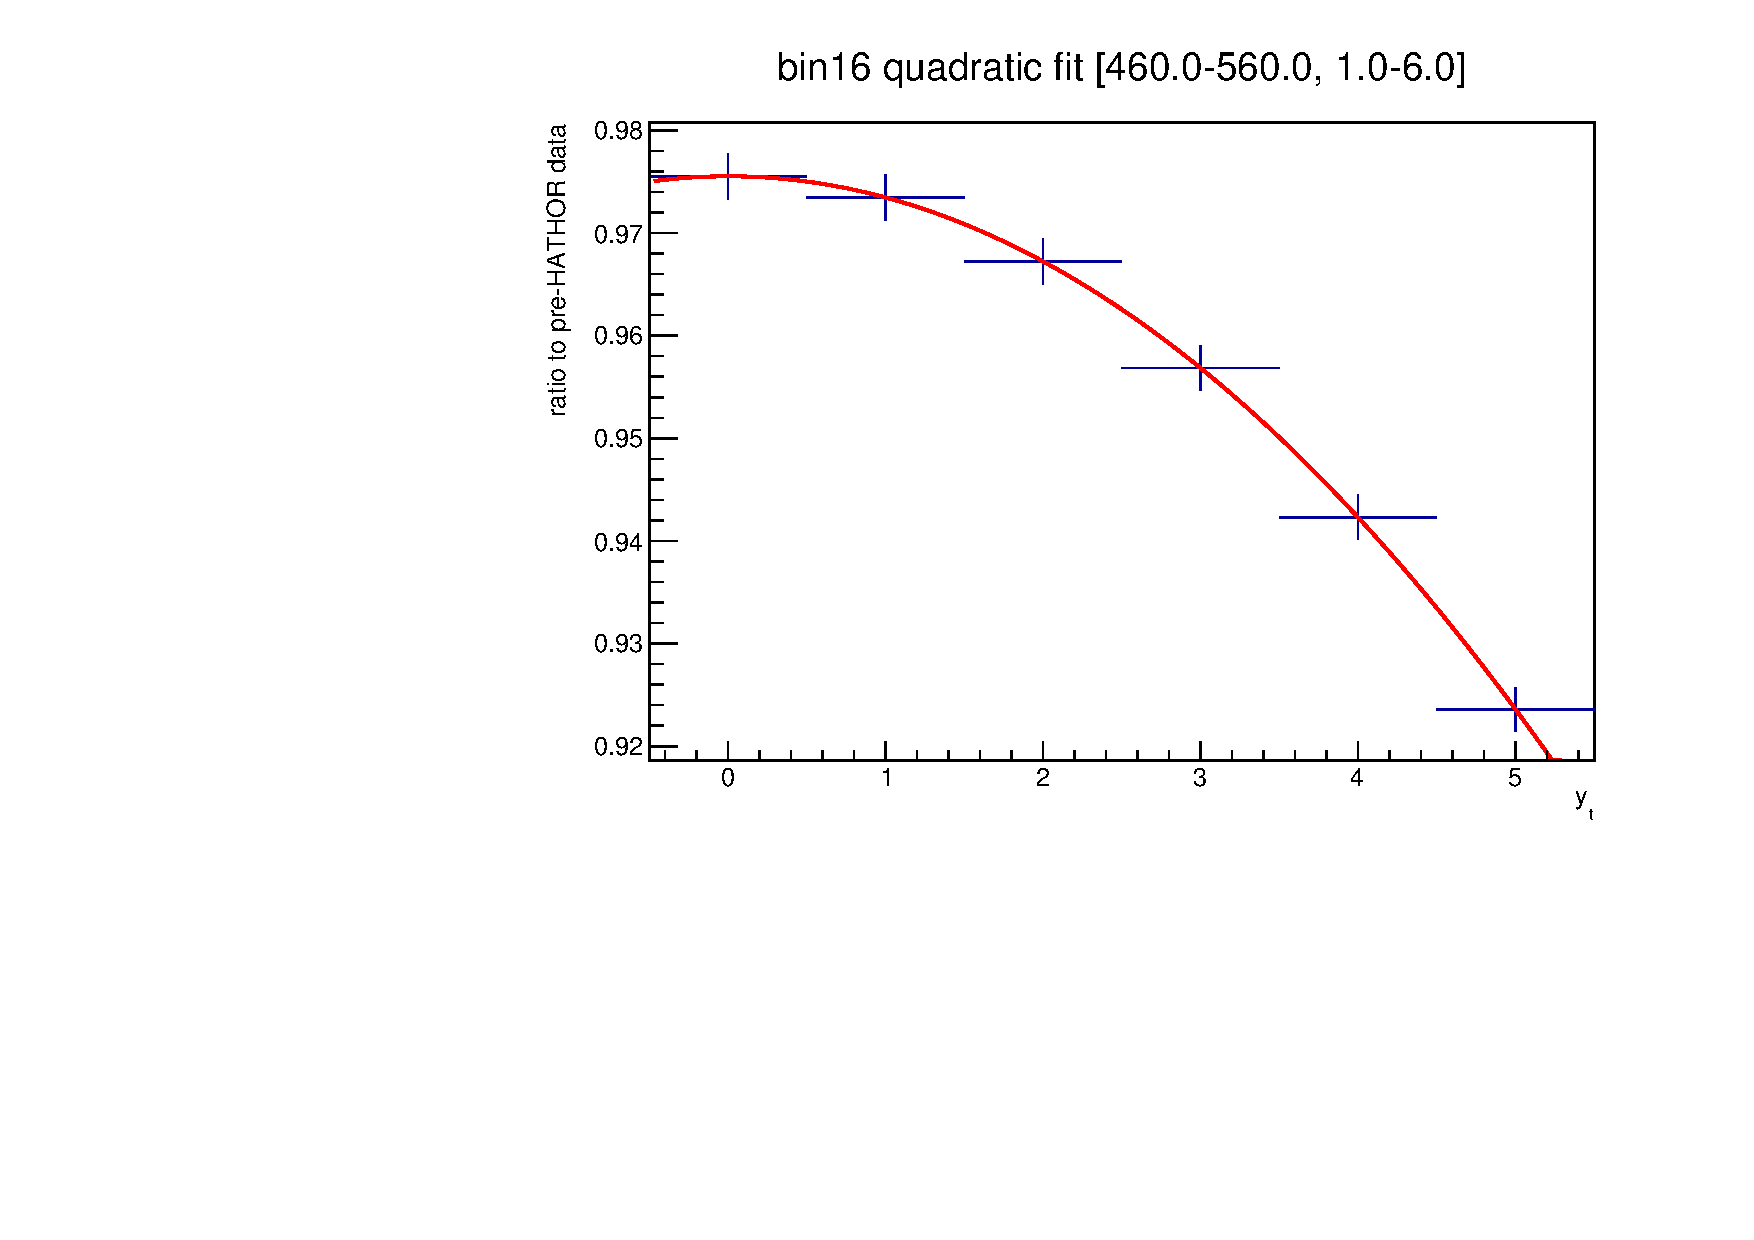
\includegraphics[width=.48\linewidth]{quadplots/2017bin16.pdf}

 \caption{The EW correction weights in two separate [$\Mbl, \DYbl$] bins, demonstrating the quadratic dependence on $\yt$. The full set of bin-by-bin EW corrections is shown in Appendix \ref{S:bins}}
    \label{fig:quad}
\end{figure}

\clearpage
\section{Sources of uncertainty}

The list of uncertainties considered is very similar to that of the analogous measurement using 2016 data in \cite{ytnote}. The main differences are the lack of QCD multijet background and the  use of the full run 2 dataset. Some uncertainty sources are evaluated differently in the 2017-2018 Monte Carlo samples compared to the 2016 sample. In this section we first give a brief overview of each uncertainty source, then we comment on the processing of systematic templates and their correlation between data set corresponding to different years.

\label{S:sys}
\subsection{Experimental uncertainty sources}
\label{SS:syslist}

\noindent \textbf{Luminosity (lumi)}

The overall uncertainty in integrated Luminosity is included as a scale uncertainty applied to signal and background events. The value of the uncertainty comes from the Lumi POG \cite{LumiTwiki}.

\par \noindent
\textbf{Pileup (pu)}

Pileup reweighting is applied to adjust the number of interactions generated in the Monte Carlo to match the data. The inelastic cross section, 69.2\unit{mb}, is varied by $1\sigma = 4.6\%$ to estimate the uncertainty from this reweighting.

\par \noindent
\textbf{Jet Energy Scale (JES\_$\ast$)}

Each individual source of uncertainty on the JES corrections, as recommended by the JetMET POG \cite{JECtwiki}, is considered as a shape uncertainty in each year. They are subjected to the pre-fit processing outlined in \ref{SS:processing}, and thus do not all appear in the final fit.

\par \noindent
\textbf{Jet Energy Resolution (JERup, JERdown)}

The Jet Energy Resolution is observed to be worse in data than in Monte Carlo. To account for this, a smearing is applied according to the recommendation of the JetMET POG \cite{JERtwiki}. The uncertainty on this procedure is modeled by shifting the desired final resolution (as a function of $\eta$ and $p_T$) by $\pm 1\sigma$ as supplied by the current JetMET POG.
Because this uncertainty affects both the jet selection and the event reconstruction, the resulting shape template is found to be highly asymmetric and often one-sided. To address this, we split the JER systematic into two systematics, up and down, which are then each symmetrized as described in Section~\ref{SS:processing}. This procedure ensures a conservative approach, which allows for full consideration of the possible shape impacts that the JER template might yield, while also ensuring stable performance of the Combine fit.

\par \noindent
\textbf{MET}

The missing transverse momentum, or MET, is affected by the uncertainty on jet energy. However, there is also some systematic uncertainty on the MET due to the energy scales of particles which are not reconstructed as part of a jet, which affects both  the MET resolution and the MET scale.

While  this uncertainty was found to be negligible in reconstructing semi-leptonic decays, it is increased in the dilepton channel when attempting a full kinematic reconstruction, due to the nonlinear dependence of neutrino solutions on the MET. This is one of the reasons why we opted to leave out neutrinos. The MET uncertainty now only enters our analysis as a negligible effect on the same-flavor lepton decays, where a MET-based selection is used.

\par \noindent
\textbf{Lepton scale factor (eltrg, elrec, mutrg, murec)}

A scale factor is applied to correct for efficiencies of lepton reconstruction, ID, isolation, and triggers. This scale factor, and it's inefficiencies, are evaluated using the tag-and-probe technique on $Z$ boson decays. As we use single lepton triggers, this uncertainty must be split into two uncertainties for each lepton flavor (mu/el), which we label rec (reconstruction+ID+iso) and trg (trigger).

\par \noindent
\textbf{$b$-tagging and mis-tagging (btag, ltag)}

To account for discrepancies in the b-tagging and mis-tagging efficiencies between data and Monte Carlo, scale factors are applied to each jet. These factors are varied up and down by $1\sigma$ to estimate the corresponding uncertainty.

\par \noindent
\textbf{Prefire }

An uncertainty is included on the weights generated to address the L1 pre-fire problem in the ECAL in 2016 and 2017.

\subsection{Theoretical uncertainty sources}


\noindent \textbf{Renormalization and factorization scales (rs, fs, rsfs)}

The QCD renormalization and factorization scales are each varied up and down in the Monte Carlo by a factor of 2, as a standard technique to estimate uncertainty due to higher-order QCD terms.

This standard practice is meant to account for contributions from higher order QCD terms to the Monte Carlo. While it does a decent job of estimating the potential magnitude of these corrections, it is a rather imprecise way of estimating their possible shape, to which this analysis is sensitive. To help capture a greater variety of possible shape distortions coming from higher order terms, we include a same sign variation, rsfs, in which the two scales are varied simultaneously (same sign variation).

Since we normalize the cross section to the NNLO value, we remove the overall normalization effect from all scale variation uncertainties, which otherwise would be overestimated. 
%If including the normalization component, this would result in an overestimate of total uncertainty. However, we remove , as . From a shape-based perspective, the same sign variation is a perfectly valid candidate for higher order effects. 

\par \noindent
\textbf{Uncertainty due to Electroweak (HATHOR) correction} 

We include an uncertainty on the EW corrections, based on our methods for generating and applying these additional terms, as outlined in Sections \ref{SS:kfactor} and \ref{SS:statmeth}.

Like the scale variations, this uncertainty stands in for higher-order effects, predominantly those coming from diagrams of order $\alpha_s^3 \alpha$. 
%It should be possible in the near future to examine these terms directly, although it is not clear if this will be achievable in the timespan of this analysis due to tight schedule constraints.

\par \noindent
\textbf{PDFs (pdf\_i, pdf\_alpha)}

We use the NNpdf set \cite{NNPDF}, which contains 100 individual variations as uncertainty sources.  We follow the technique described in \cite{ytnote} to reduce the number of variations to 10 templates. These uncertainties are then subject to the pre-fit processing (Section \ref{SS:processing}), so they do not all appear in the final fit. We also note that these uncertainties are treated as fully correlated between 2017/2018 datasets, but not in the 2016 MC where they were generated differently.
The effect of the value of the strong coupling $\alpha_s$ used by NNpdf is included and treated separately from the other pdf variations.

\par \noindent
\textbf{Top mass (mtop)}

Dedicated Monte Carlo samples are generated with the top mass varied up and down by 1 \unit{GeV} to estimate the effect of the top mass uncertainty. 

\par \noindent
\textbf{Matrix element / parton shower matching (hdamp)}

The $h_{damp}$ parameter, which controls the matrix element parton shower matching in \small\textsc{POWHEG + PYTHIA8}, is set to the nominal value of $h_{damp}= 1.58 \cdot m_\mathrm{t}$. Dedicated Monte Carlo samples are generated with this parameter varied down to $1 \cdot m_\mathrm{t}$ and up to $2.24 \cdot m_\mathrm{t}$, in order to estimate the effect of this uncertainty.

\par \noindent
\textbf{Monte Carlo tune / underlying event (tune)}

Dedicated Monte Carlo samples are generated with variations of the PYTHIA tune in order to estimate the effect of modeling the underlying event.
\par \noindent
\textbf{Initial and final state radiation (isr, fsr)}

Uncertainty due to initial and final state radiation is assessed by varying the value of the strong coupling $\alpha_\mathrm{s}$ up and down in the parton shower algorithm, in the initial and final states, respectively. In 2016 this was done using dedicated Monte Carlo samples. The effect in these samples was thought to be unrealistically large, so the effects are scaled down by a factor of $1/\sqrt{2}$ for this year, following the prescription in \cite{Skands:2014pea}. In 2017 and 2018, the uncertainty was implemented via weights in the central Monte Carlo sample. We use the weights corresponding to a variation of $\alpha_\mathrm{s}$ by a factor of 2.

\par \noindent
\textbf{$b$-jet fragmentation (bfrag)} 

The momentum transfer from $b$ quarks to $B$ hadrons is modeled with a transfer function dependent on $x_b=\frac{p_T(B)}{p_T(b-jet)}$. To estimate the uncertainty, the transfer function is varied up and down by 1$\sigma$ of the Bowler-Lund parameter in PYTHIA8. The resulting effect is applied via weights.


\par \noindent
\textbf{B decay branching (bdec)} 

The b-jet response is sensitive to the branching ratio of semi-leptonic B decays. Samples are reweighted with this branching fraction varied up and down by 1$\sigma$ according to the PDG value of the uncertainty. 

\par \noindent
\textbf{Signal and background normalization (tt\_norm, st\_norm, vj\_norm)} 

A 10\% normalization uncertainty is included on the \ttbar sample, meant to represent the normalization effects of scale variations, which have been subtracted from their templates. This is admittedly an overestimation, but we should not be very sensitive to normalization effects, so it is included presently as a check on the fit.

The backgrounds in this analysis are small enough ($\approx$2\% sample composition each) that we do not generate templates for their response to individual systematic uncertainties. Instead, a 15\% normalization uncertainty is included on each.




\subsection{Pre-fit processing of systematics}
\label{SS:processing}

\begin{figure}
    \centering
    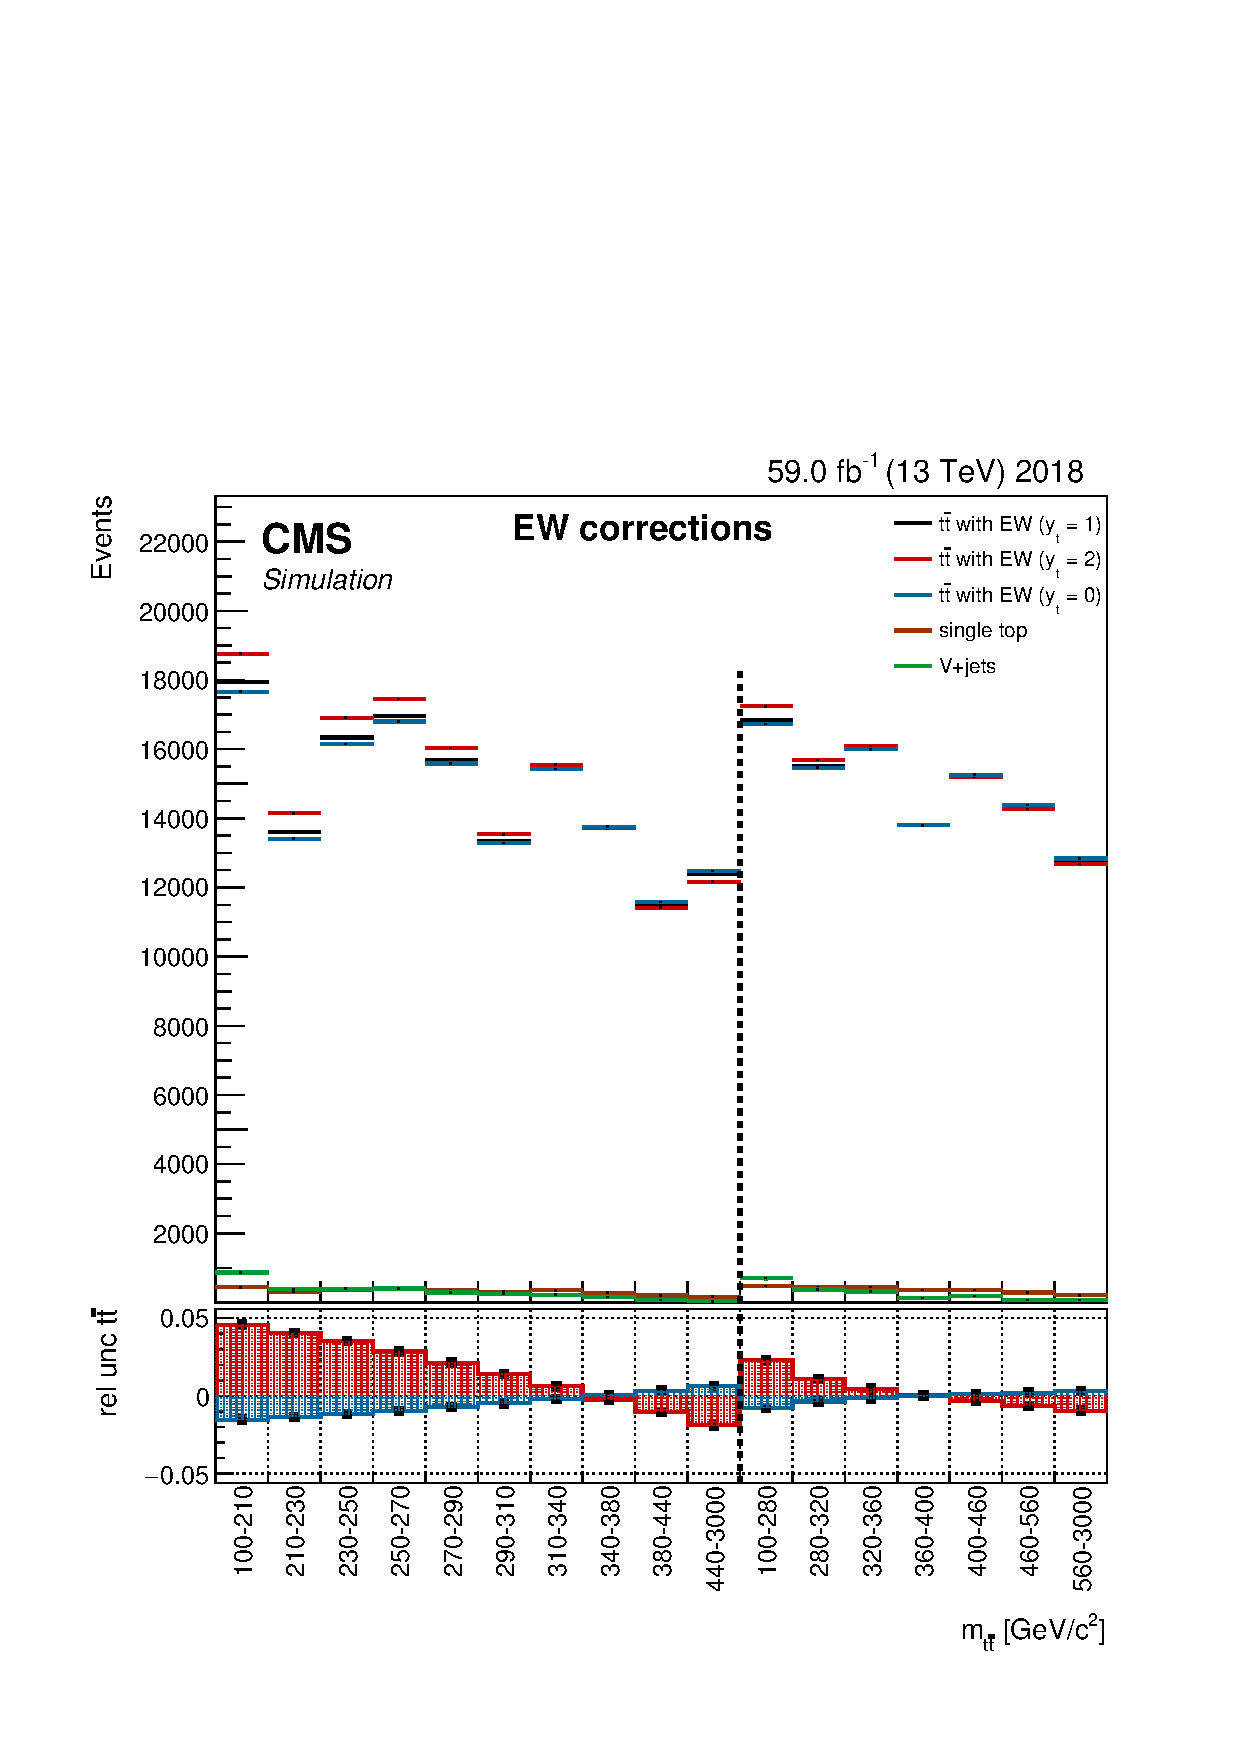
\includegraphics[width=0.8\linewidth]{templates/yuk.pdf}
    \caption{The effect of the yukawa parameter \yt on binned reconstructed events. We see that the effect induces a shape distortion on the kinematic distributions not unlike a systematic uncertainty template.}
    \label{fig:yuktemplate}
\end{figure}


In this analysis, the POI, $\yt$, manifests itself as a smooth shape distortion of the kinematic distributions as seen in Figure \ref{fig:yuktemplate}. This behavior lessens the effect of normalization systematics, but also means we must take extra care in handling the shape systematics. Many sources of systematics are described by templates with significant variations (see Appendix \ref{S:templates}). While these variations can be genuine, more frequently they are due to fluctuations in the dedicated Monte Carlo samples with low statistics or other issues involving a lack of available information. These systematic uncertainties will typically be over-constrained by the likelihood fit while having little impact on the POI. As a result their potential impact on the POI could be  vastly underestimated. We thus attempt to smooth out fluctuations in our systematic templates which allow a better estimate of their potential effects on the measurement by assuming that they arise from some smooth distribution like the POI.

Specifically, smoothing is applied to the \Mbl shape in each \DYbl\, bin after binning and forming the marginal templates as shown in Appendix \ref{S:templates}. Since the bins are chosen to have similar statistics, this procedure closely mirrors the outcome of a variable-width smoothing done based on statistical uncertainties in a fixed-width binning. 
%Attempts to employ a fixed width binning on the \Mbl spectrum yielded nonsensical results at high \Mbl values where statistics are low.

We employ a weighted moving average smoothing technique. If the input bin values are $\{b_i\}$, the value of a given bin after smoothing is 

\begin{equation}
    B_i = \frac{ \sum_{j=1}^N w_j\cdot b_j}{\sum_{j=1}^N w_j},\quad\quad
    w_i = \exp{\left[\frac{-|i-j|}{2s}\right]}.
    \label{eq:smooth}
\end{equation}
The parameter $s$ determines the width of the smoothing. Rather than assign it arbitrarily, we attempt to calculate a measure of ''roughness" of the template beforehand. To do this, we first smooth the bins $b^\mathrm{in}_i$ with smoothing width $s=2$ to obtain $b^\mathrm{out}_i$. We  define an average magnitude of the template $b$ to as $\mathrm{mag}(b) = \frac{1}{N}\sum_{i=1}^N |b_i|$. We then calculate the average marginal change in the template's bin content, defining the statistic:

\begin{equation}
\zeta = \frac{1}{N}\sum_{i=0}^N  \frac{|b^\mathrm{in}_i-b^\mathrm{out}_i|}{\mathrm{mag}(b)}.
\end{equation}

The parameter $\zeta$ is a measure of the smoothness of a certain systematic and its potential impact on the POI. 
The value of $\zeta$  generated by the POI itself is consistently less than 0.1. 
%On the other hand, some systematics are quite noisy and yield much larger values. These systematics are found to have erratic, often underestimated effects on the fit, meanwhile often typically over-constrained. If large, they can also affect the stability of the fit, by creating a very jagged likelihood function. 
%To remedy this, 
If a systematic uncertainty template with binned values $\{b_i\}$ yields a parameter $\zeta>0.25$, we choose to smooth it using Eq.~\ref{eq:smooth} with a width of $s=4 \zeta$. This value typically results in smooth templates that consistently provide a more stable fit and with a more conservative result.

Since the POI template is asymmetric  it is not surprising that even slightly asymmetric systematics can yield a one-sided impact on $\yt$. This generally ill-regarded phenomenon can be remedied by symmetrizing the systematic templates. After smoothing, the ``down" template is negated and compared to the ``up" template. In each bin, the  value with the largest magnitude is taken to generate a new ``up" templates, which is given a symmetric ``down" template. This is found to yield a slightly more conservative sensitivity in the fit, while helping the convergence of the fit as well as avoiding some one-sided impacts. 

Lastly, systematics which are extremely small ($<0.1\%$ effect in msot bins) or extremely noisy (tune, hdamp) are flattened and included together in an overall normalization uncertainty. 

All systematic templates are shown before and after processing in Appendix \ref{S:templates}.



\subsection{Correlation of systematics across run 2 datasets}
\label{SS:corr}


In our treatment of systematics between the three years, we allow the possibility that systematics are uncorrelated, fully correlated, or partially correlated between years. 
Whenever possible we follow the recommendation of the appropriate POG, which exist for the following uncertainties:
\begin{itemize}
    \item Luminosity, from the Lumi POG \cite{LumiTwiki};
    \item Jet energy correction and resolution, from the JETMET POG \cite{JECtwiki}.
\end{itemize}
The correlation factors for the remaining systematic uncertainties are summarized in Table \ref{tab:run2corr}  and detailed below.

\par \noindent
\textbf{1. Most theory uncertainties (bkg norm, rs, fs, mtop, bdec, bfrag, EWunc)}

These uncertainties are treated as fully correlated between all 3 years. They are underlying theoretical uncertainties with well-behaved templates, and  no well-motivated reason to change from year to year. 

The mtop template is a bit special, as there are limited statistics in the dedicated MC samples, making it difficult to extract a meaningful shape in each individual year (Fig. \ref{fig:mtop_template_old}). 
%However, we could see that the three years had some common features, muddled by statistical noise. 
By combining the samples for all three years, we are able to extract a more sensible shape template (Fig. \ref{fig:mtop_template}).

\par \noindent
\textbf{2. Theory uncertainties for which modeling was changed after 2016 (isr,fsr,pdf\_$\ast$)}

%The means by which these uncertainties were modeled changed after 2016. 
ISR and FSR uncertainty implementation switched from dedicated MC samples to weights, which had a significant effect on their magnitudes. The version of NNpdf implemented in the nominal MC sample was also changed, and the individual variations are unrelated between versions, making it impossible to correlate them. We thus treat these uncertainties as fully correlated between 2017-2018, but leave the 2016 values as uncorrelated from other years.

% \par \noindent
% \textbf{3. Overconstrained theory uncertainties (bfrag)}

% In principle, the change in MC tune after 2016 could partially de-correlate some theory systematics in this year from the other years. Since most theory systematics were seen to have similar templates across all 3 years and were not overconstrained, we think this is generally not an issue. However, a possible exception is the b-fragmentation uncertainty. The template is seen to be different in 2016 from other years [ADD REF], and was seen to be overconstrained when treated as fully correlated between all 3 years. To address this, the 2016 bfrag uncertainty is now treated as 50\% correlated to other years, which resolved the overconstraint issue.

\par \noindent
\textbf{3. Very noisy theory uncertainties (tune, hdamp)}

The nominal \ttbar MC sample in 2016 used the CUETM4 tune, which was changed to the CP5 tune in subsequent years. In principle, these systematics might belong to the previous category. In practice, they come from dedicated MC samples which result in templates consisting largely of statistical noise. These are flattened by our systematics processing in Section \ref{SS:processing}. The resulting values are considered uncorrelated due to the large amount of statistical noise, and are flattened in the systematics processing step anyhow.

\par \noindent
\textbf{4. Experimental scale factor uncertainties (btag, ltag, eltrg, elrec, mutrg, murec)}

Based on discussions with members of the BTV POG, and our own experience with the lepton scale factor code, we believe that a significant part of these uncertainties comes from the methods of calculation, rather than fluctuations in the data. We thus treat them as 50\% correlated between all years.

\par \noindent
\textbf{5. Uncertainty due to pileup}

The pileup uncertainty originates from the product of luminosity and the total inelastic cross-section. A correlated pileup uncertainty would, in principle, result from a correlated effect on the luminosity, and thus we could use the same correlation factors. However, since the pileup is a minor effect, we believe it is sufficient to treat it as 50\% correlated between all years for simplicity sake.
\begin{table}[h]
    \centering
\begin{tabular}{|l|l|l|l|}
\hline
Correlation between years:              & 16-17  & 16-18  & 17-18  \\ \hline \hline
EW correction uncertainty               & 100\%  & 100\%  & 100\%  \\ \hline
background normalization                & 100\%  & 100\%  & 100\%  \\ \hline
renormalization \& factorization scales & 100\%  & 100\%  & 100\%  \\ \hline
b decay, b fragmentation                                 & 100\%  & 100\%  & 100\%  \\ \hline
pdf uncertainties                       & 0\%    & 0\%    & 100\%  \\ \hline
ISR, FSR               & 50\%   & 50\%   & 100\%  \\ \hline
top mass                                & 100\%  & 100\%  & 100\%   \\ \hline
hdamp, MC tune *                        & 0\%    & 0\%    & 0\%    \\ \hline \hline
btag SFs, lepton SFs                    & 50\%   & 50\%   & 50\%   \\ \hline
lumi\^                                  & 30\%   & 30\%   & 30\%   \\ \hline
pileup\^                                & 50\%   & 50\%   & 50\%   \\ \hline
JER                                     & 0\%    & 0\%    & 0\%    \\ \hline
JES                                     & \multicolumn{3}{c|}{see \cite{JECtwiki}} \\ \hline
\end{tabular}
    \caption{Prescription of systematic uncertainties correlations between run 2 datasets. * Indicates sources for which correlations are motivated by limited statistics. \^\ Indicates sources for which the ideal values have been  slightly modified to allow for an easier implementation.}
    \label{tab:run2corr}
\end{table}

\subsection{Implementation of partial correlations using Combine statistics package}
\label{SS:combine}

The Combine package does not support partial correlations between years via an extra penalty term in the likelihood. Each shape or nuisance parameter automatically comes with a standard gaussian pdf. Between the different years, templates either depend on the same nuisance parameter (fully correlated) or different parameters (fully uncorrelated).

There is an easy way to overcome this missing functionality, when using only 2 years of data, which has for a while been included in a script as part of the CombineHarvester package \cite{CHscript}. This script relies on splitting a partially correlated nuisance parameter template into two separate templates, one fully correlated and the other fully uncorrelated. 

Let $\Gamma^{\mathrm{bin}}(\theta)$ be the marginal effect of a systematic uncertainty on the expected signal $s$ template on a given bin content as a function of the nuisance parameter $\theta$, which has a standard gaussian probability distribution function:
\begin{equation}
    \Gamma^{\mathrm{bin}}_\mathrm{year}(\theta) = \frac{s^\mathrm{bin}_\mathrm{year}(\theta)-s^\mathrm{bin}_\mathrm{year}(\theta = 0)}{s^\mathrm{bin}_\mathrm{year}(\theta = 0)} 
\end{equation}
\begin{equation}
    \Gamma _\mathrm{year}(\theta) = (\Gamma^1_\mathrm{year} (\theta), \ldots, \Gamma^N_\mathrm{year} (\theta))
\end{equation}

Suppose we have 2 years of data, year $a$ and year $b$. We can include partial correlations between the underlying nuisance parameters $\theta_a$ and $\theta_b$ if we split the templates $\Gamma_a$, $\Gamma_b$ into two rescaled templates:

	\begin{eqnarray}
	\Gamma_{a}(\theta_{a})\longrightarrow& \sqrt{1-\rho\,}\,\Gamma_{a}(\theta_{a}),\quad&\sqrt{\rho\,}\,\Gamma_a(\theta_\mathrm{corr}) \\
		\Gamma_{b}(\theta_{b})\longrightarrow& \sqrt{1-\rho\,}\,\Gamma_{b}(\theta_{b}),\quad&\sqrt{\rho\,}\,\Gamma_b(\theta_\mathrm{corr},)
	\end{eqnarray}

where we have introduced an additional fictitious nuisance parameter, $\theta_\mathrm{corr}$, which enforces the correlation.

This method of introducing a single fictitious nuisance parameter and rescaling the shape templates can easily be extended to a 3-year combination for simple cases, in particular when the desired correlations $\rho_{y_1,y_2}$ are the same between all 3 years: $\rho_{16,17}= \rho_{17,18} = \rho_{16,18} \equiv \rho$. In practice, this is generally the case.

The same technique can also be applied iteratively pairwise, in order to yield arbitrary correlations between the 3 years. This requires introducing 3 fictitious nuisance parameters, one for the ``correlated part" between each pair of years. At this point, the cost of introducing more parameters to the fit likely outweighs the benefits in many cases.

With this in mind, we slightly modify the recommended lumi correlations so that the lumi has the same correlation between all years. In practice, the lumi is a minor uncertainty, and the correlations between years are similar, ranging from 20\%-30\%. We believe the values in Table \ref{tab:run2corr} are sufficient.

\clearpage
\section{Sensitivity Study}
\label{S:fit}
To study the expected sensitivity of our measurement of $\yt$, we perform a maximum likelihood fit using the Asimov dataset with $\yt=1$. The fit results in a 60\% CI of [.58,1.31], and a 95\% CI of [0,1.56]. The impacts of the leading nuisances are shown in Figure~\ref{fig:impacts}, while a scan of the negative log likelihood as a function of $\yt$ is shown in Figure~\ref{fig:scan} (left). The result is comparable to the measurement obtained in \cite{ytpaper}, and the fit seems well-behaved.

The overall health of the fit appears good, with a few minor issues. A few nuisances are constrained by the fit in Figure \ref{fig:impacts}, but most of these have a sensible explanation. 
\begin{itemize}
    \item scale variations (rs, fs, rsfs)
    
    These come from rule-of-thumb scale variations meant to account for potential effects of higher order QCD terms. Because they do not arise from a normal uncertainty computed at $\pm 1 \sigma$, they are often seen to be constrained. This does not indicate a problem with the fit, but rather reflects the imprecision inherent in trying to estimate higher-order physics contributions.
    
    The one-sided impact of the same-sign variation rsfs likely arises from its unusual shape. Comparing the shape of rsfs variations to that of the POI, it is not clear what impact one should expect, and it could be that the up and down variations lead to very distant minima in the parameter space of the fit. This probably warrants some further investigation to clarify.
    
    \item EWunc
    
    This is already thought to be an overestimate, so its overconstraint is not surprising. 
    %However, it could also come from incorrect modelling.
    
    \item mtop
    
    Given that extra processing was required to extract a reasonable top mass template (see Figures \ref{fig:mtop_template_old},\ref{fig:mtop_template}), and that all 3 years are forced to have exactly the same template, this is not too surprising. The variation of $\pm 1$GeV is also not statistically motivated in a precise sense, so it is difficult to say whether this constraint is genuine, or an artifact of template smoothing and combination. 
    
    \item ttnorm
    
    This uncertainty is known to be overestimated in the current fit. Over-constraint here is thus expected, and this parameter could be reduced to a more realistic value in the final version. However, we think the inclusion of a large normalization uncertainty on ttbar is informative, as we should not be too sensitive to such an effect.
    
    \item fsr
    
    The slight overconstraint of the FSR could be due to the contribution from 2016 samples, where FSR is known to be significantly overestimated. New 2016 samples with weighted variations of the FSR have been generated, which we plan to implement in early 2020 to improve this uncertainty.
    
    \item bfrag
    
    While we initially thought this was due to the difference in 2016 templates (see Figure \ref{fig:bfrag_template}), partially decorrelating the 2016 bfrag uncertainty was not seen to improve the over-constraint. This may require some further investigation.
    
    
\end{itemize}


\begin{figure}
    \centering
    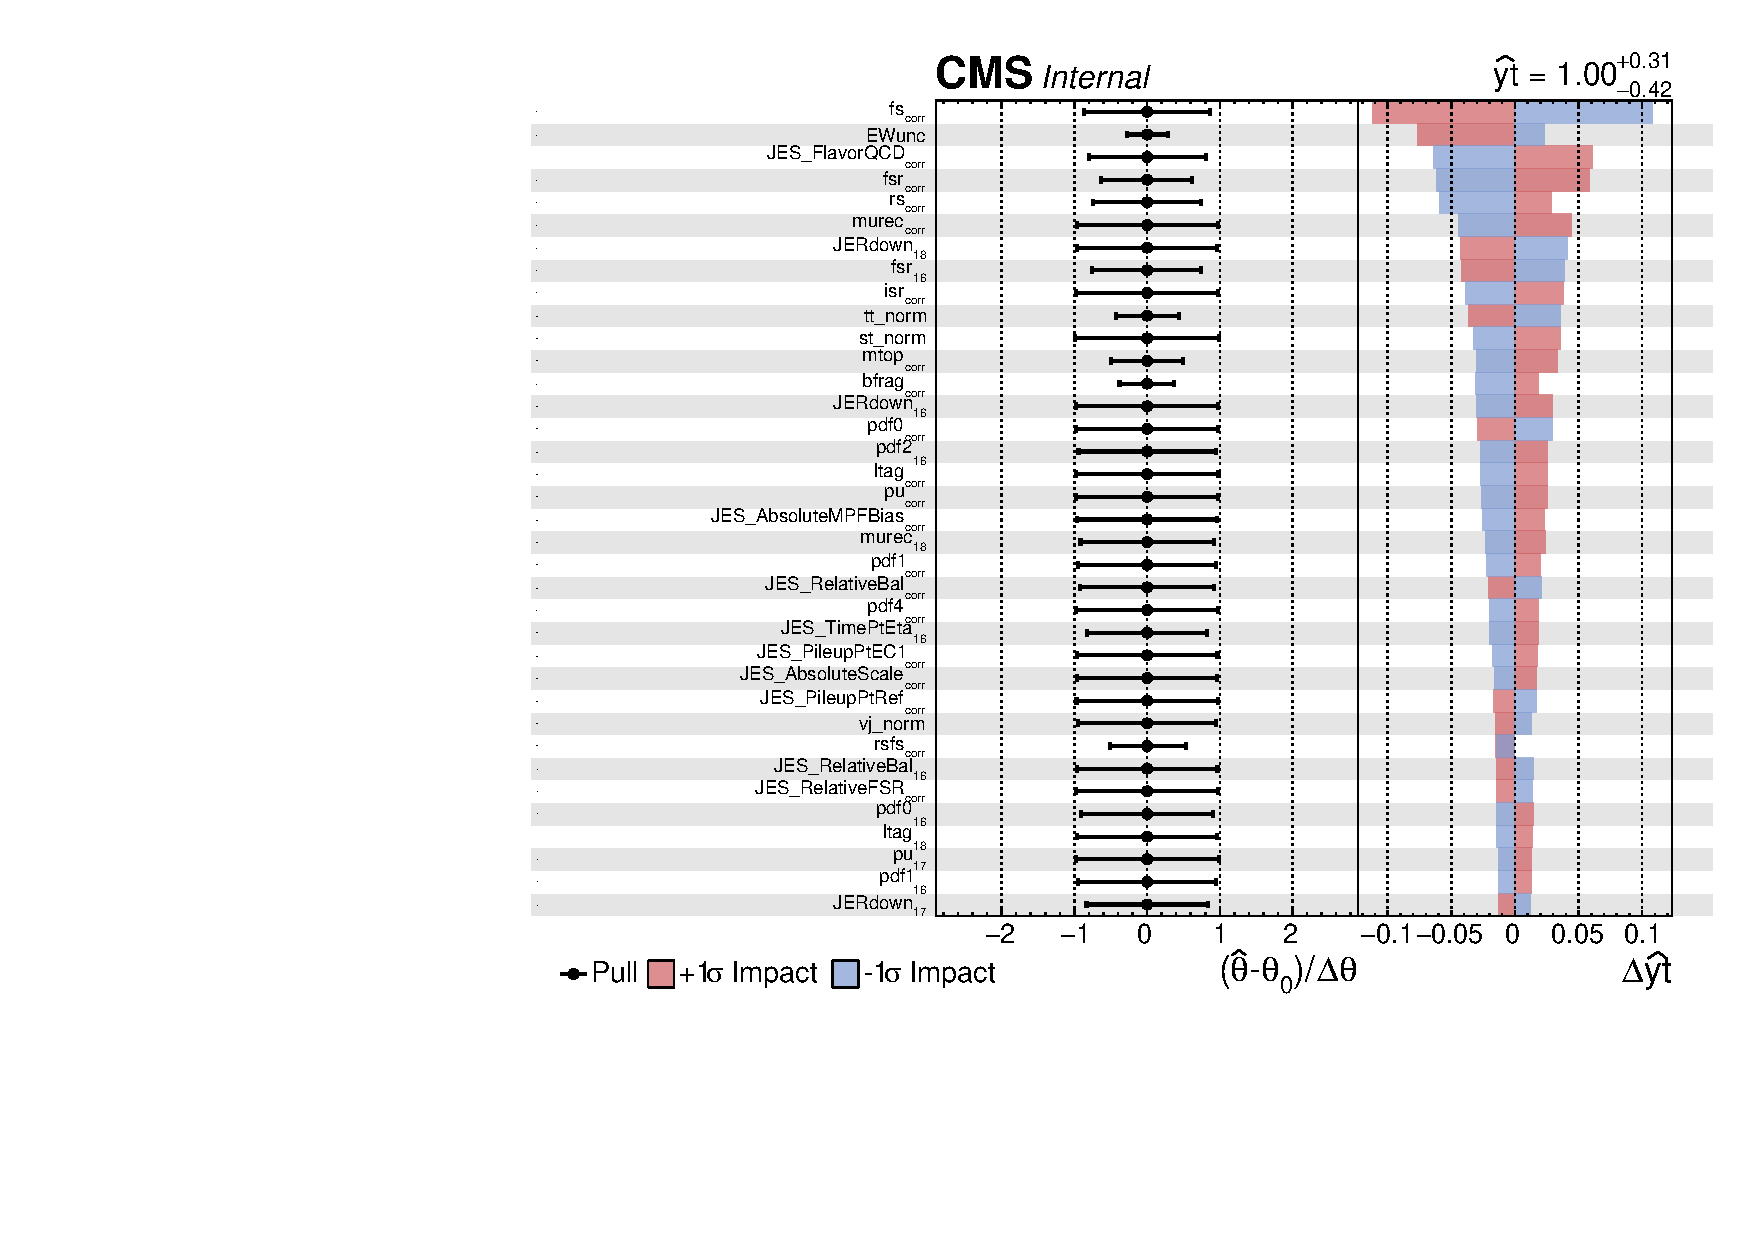
\includegraphics[width=.98\linewidth]{figs/impacts1.pdf}
    \caption{Impacts of systematics on the best fit value for $\yt$ using the Asimov data set. For brevity, only the leading 34 systematics are shown. See Appendix \ref{S:fullimpacts} for all impacts}
    \label{fig:impacts}
\end{figure}



\begin{figure}
    \centering
    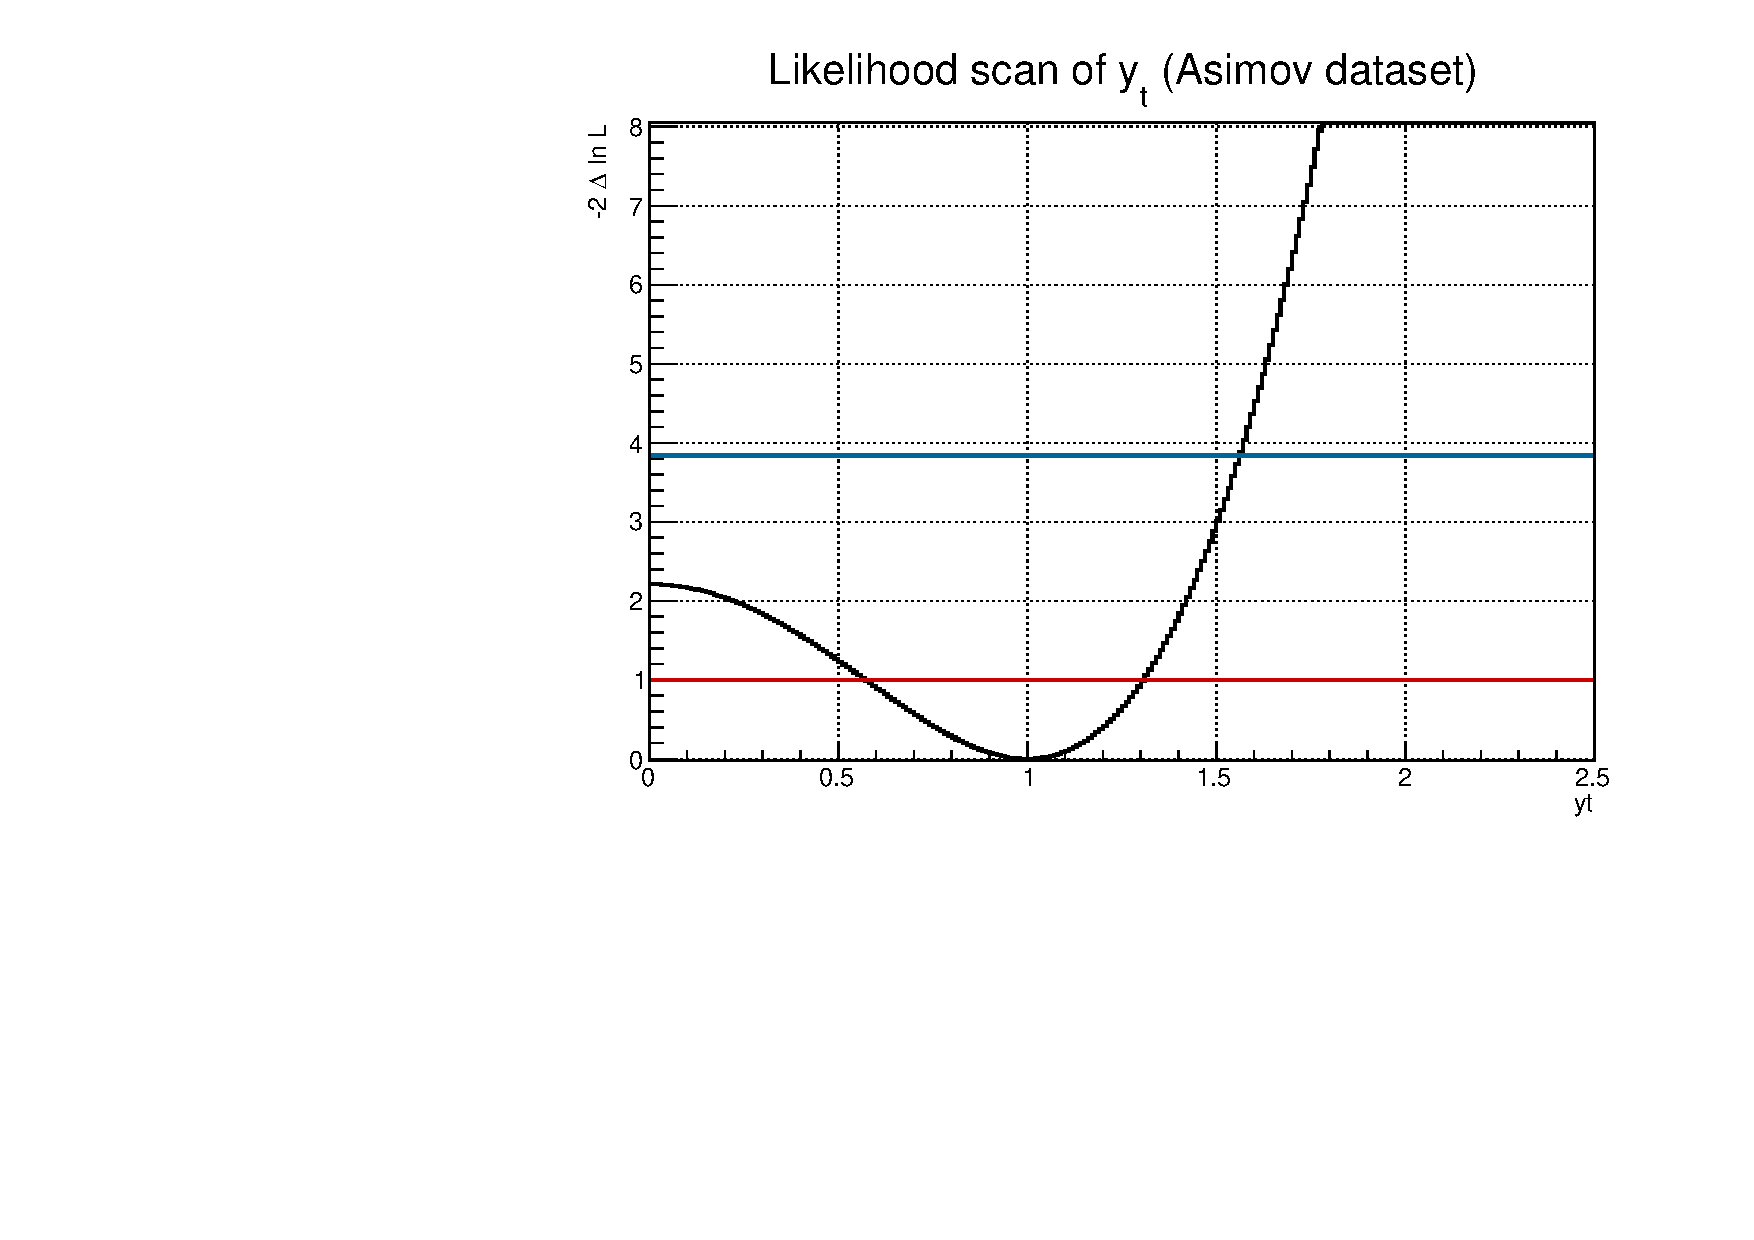
\includegraphics[width=.49\linewidth]{figs/myLL.pdf}
    \caption{The result of a likelihood scan, performed by fixing the value of $\yt$ at values over the interval [0,2.5] and minimizing the negative log likelihood (NLL). } 
    \label{fig:scan}
\end{figure}



\clearpage


\section{Conclusions}
\label{S:conc}
shit sucks

\appendix

\section{Bin sensitivities to EW corrections}

\begin{figure} \centering
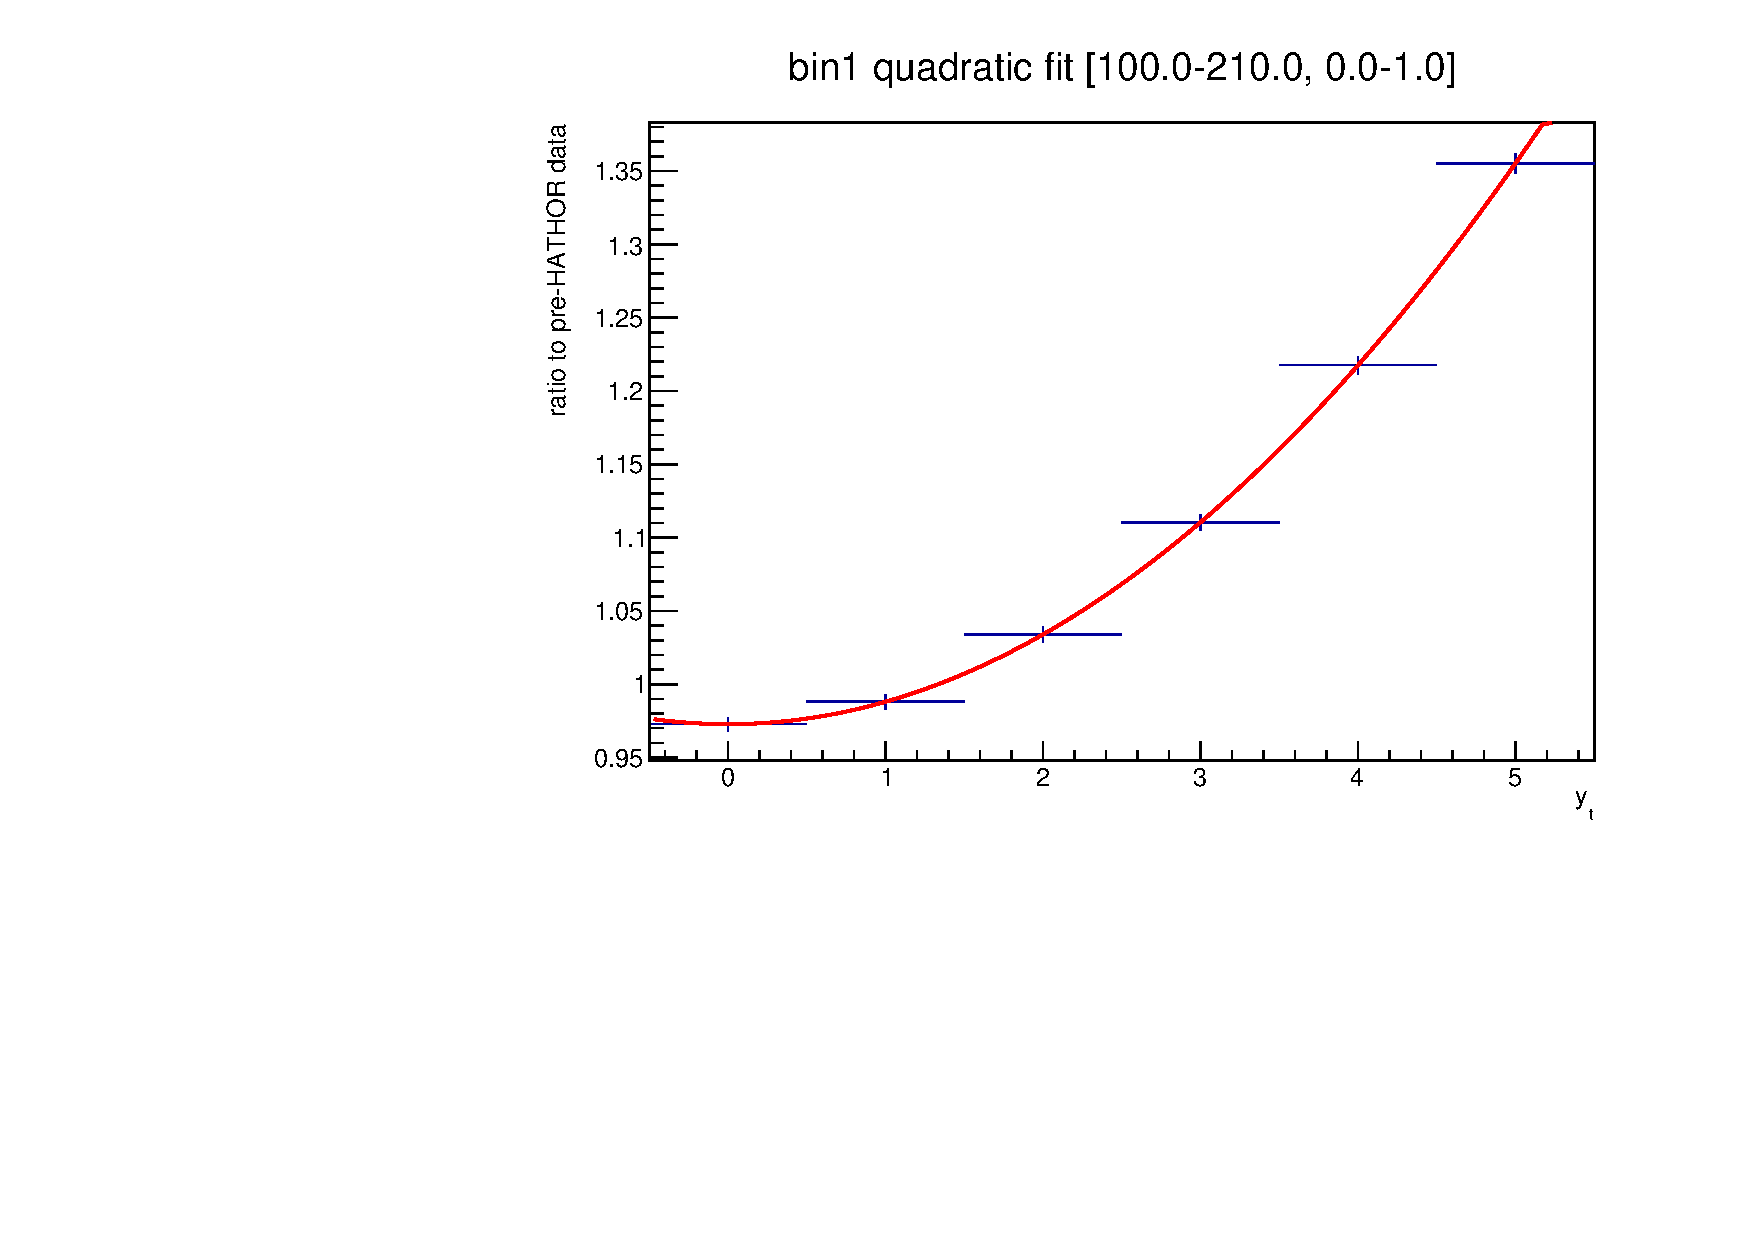
\includegraphics[width=.32\linewidth]{quadplots/2016bin1.pdf}
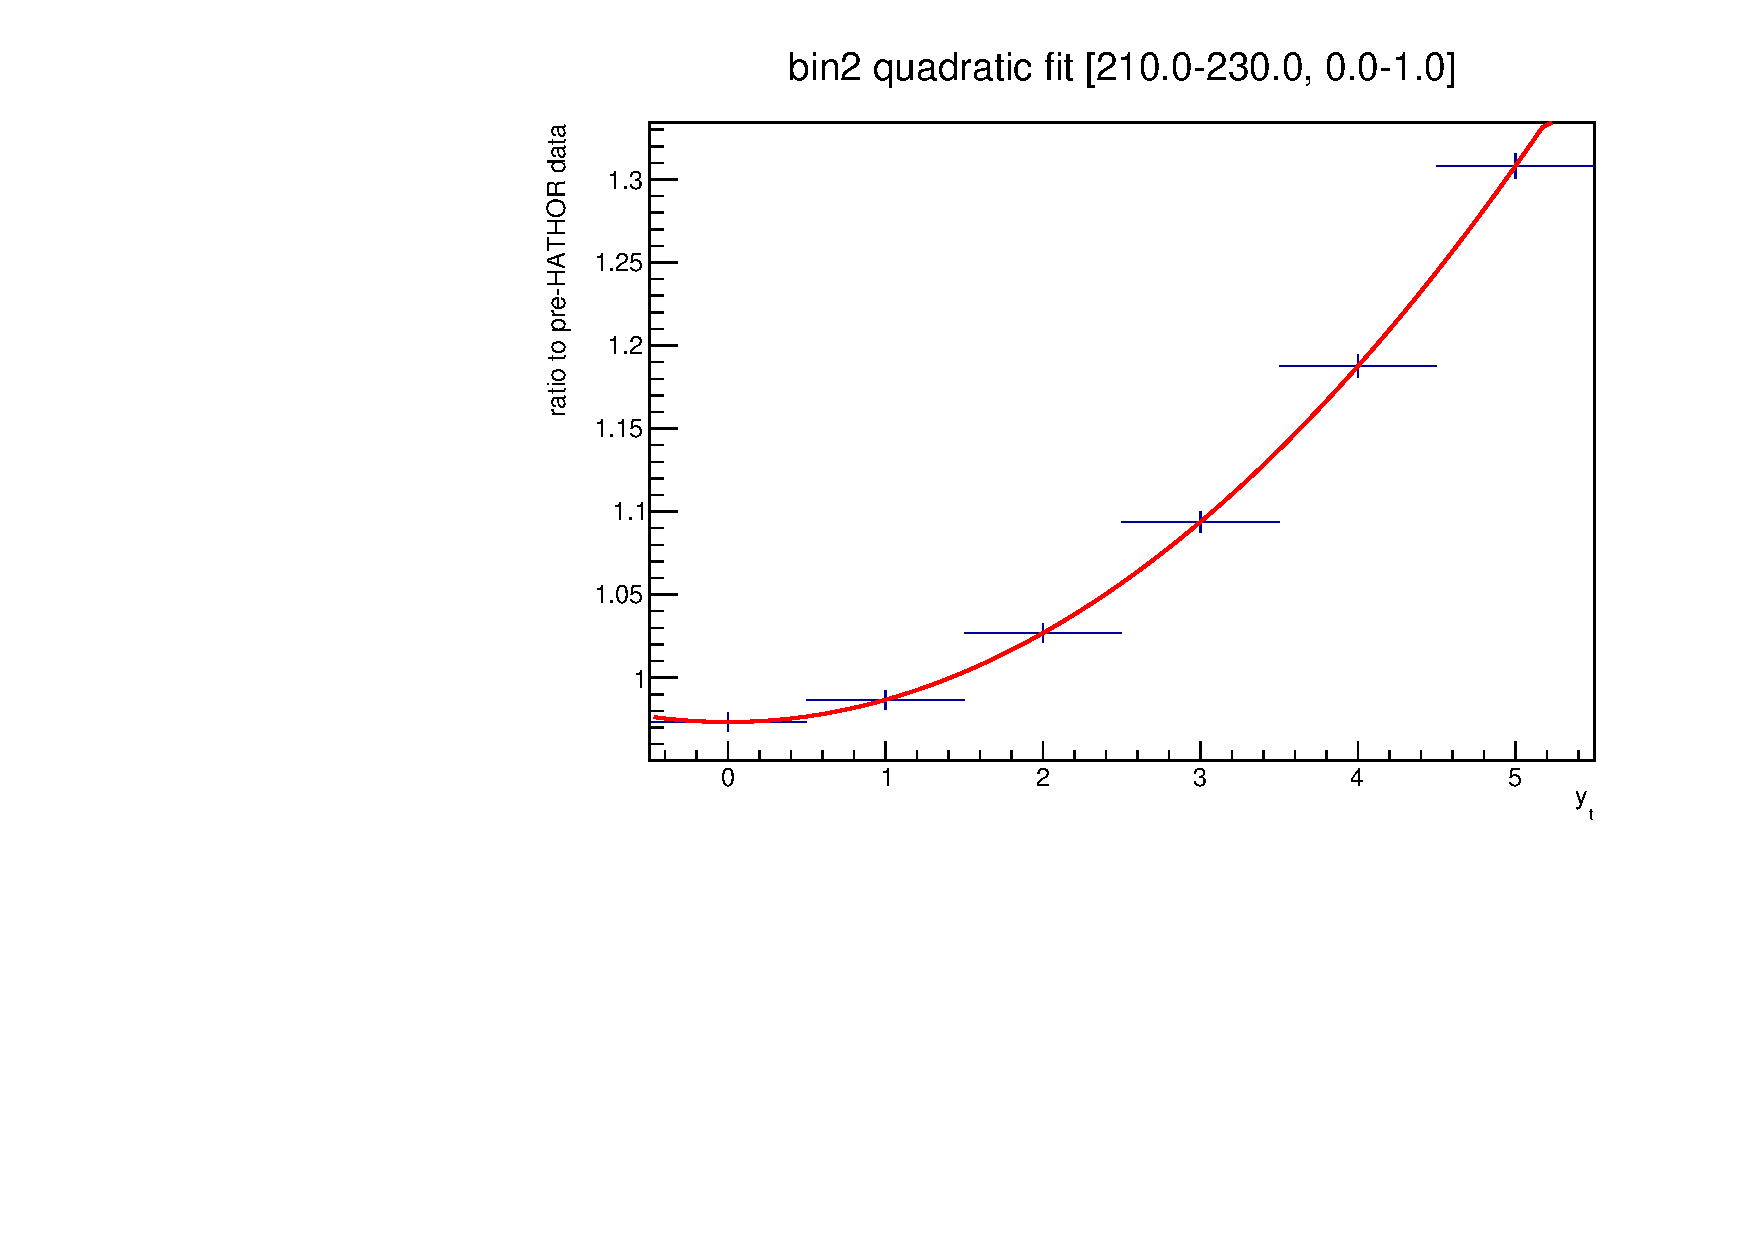
\includegraphics[width=.32\linewidth]{quadplots/2016bin2.pdf}
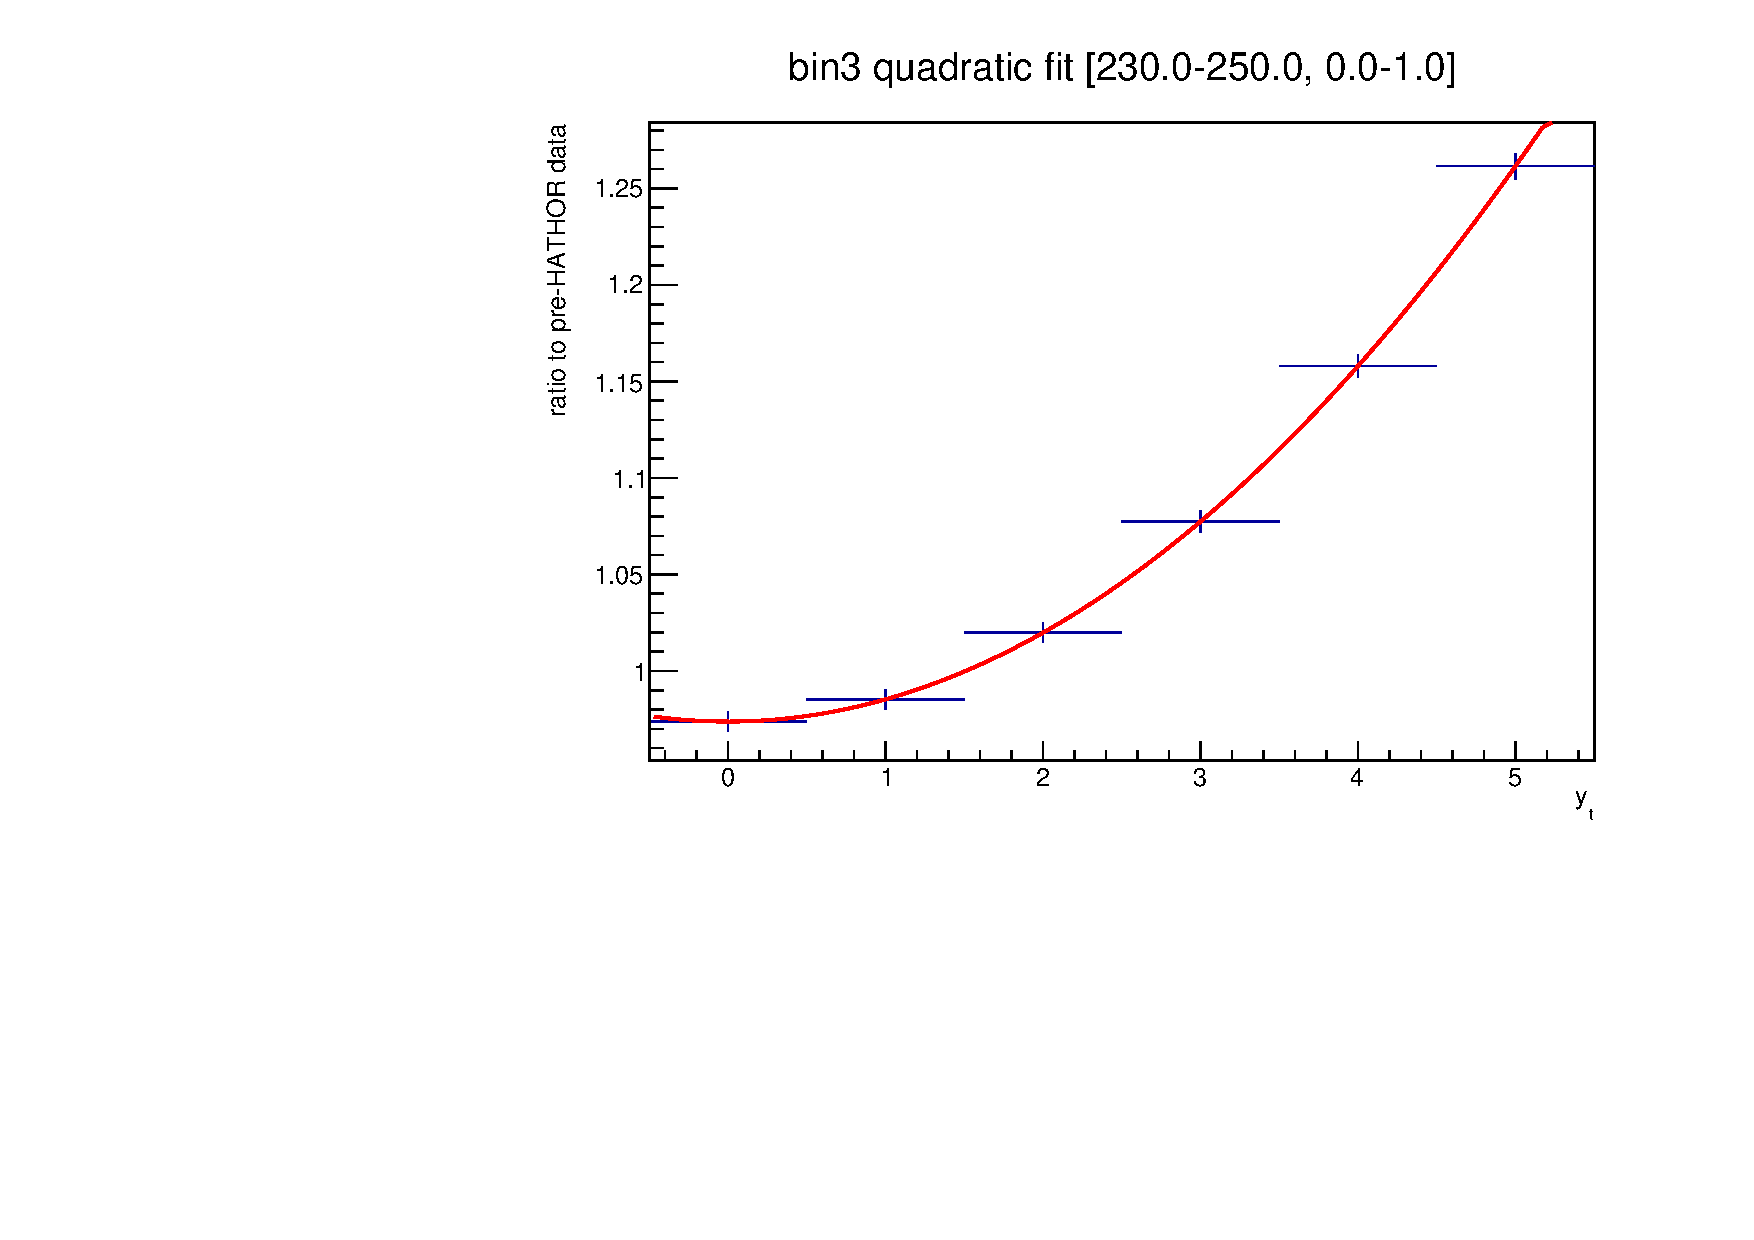
\includegraphics[width=.32\linewidth]{quadplots/2016bin3.pdf}
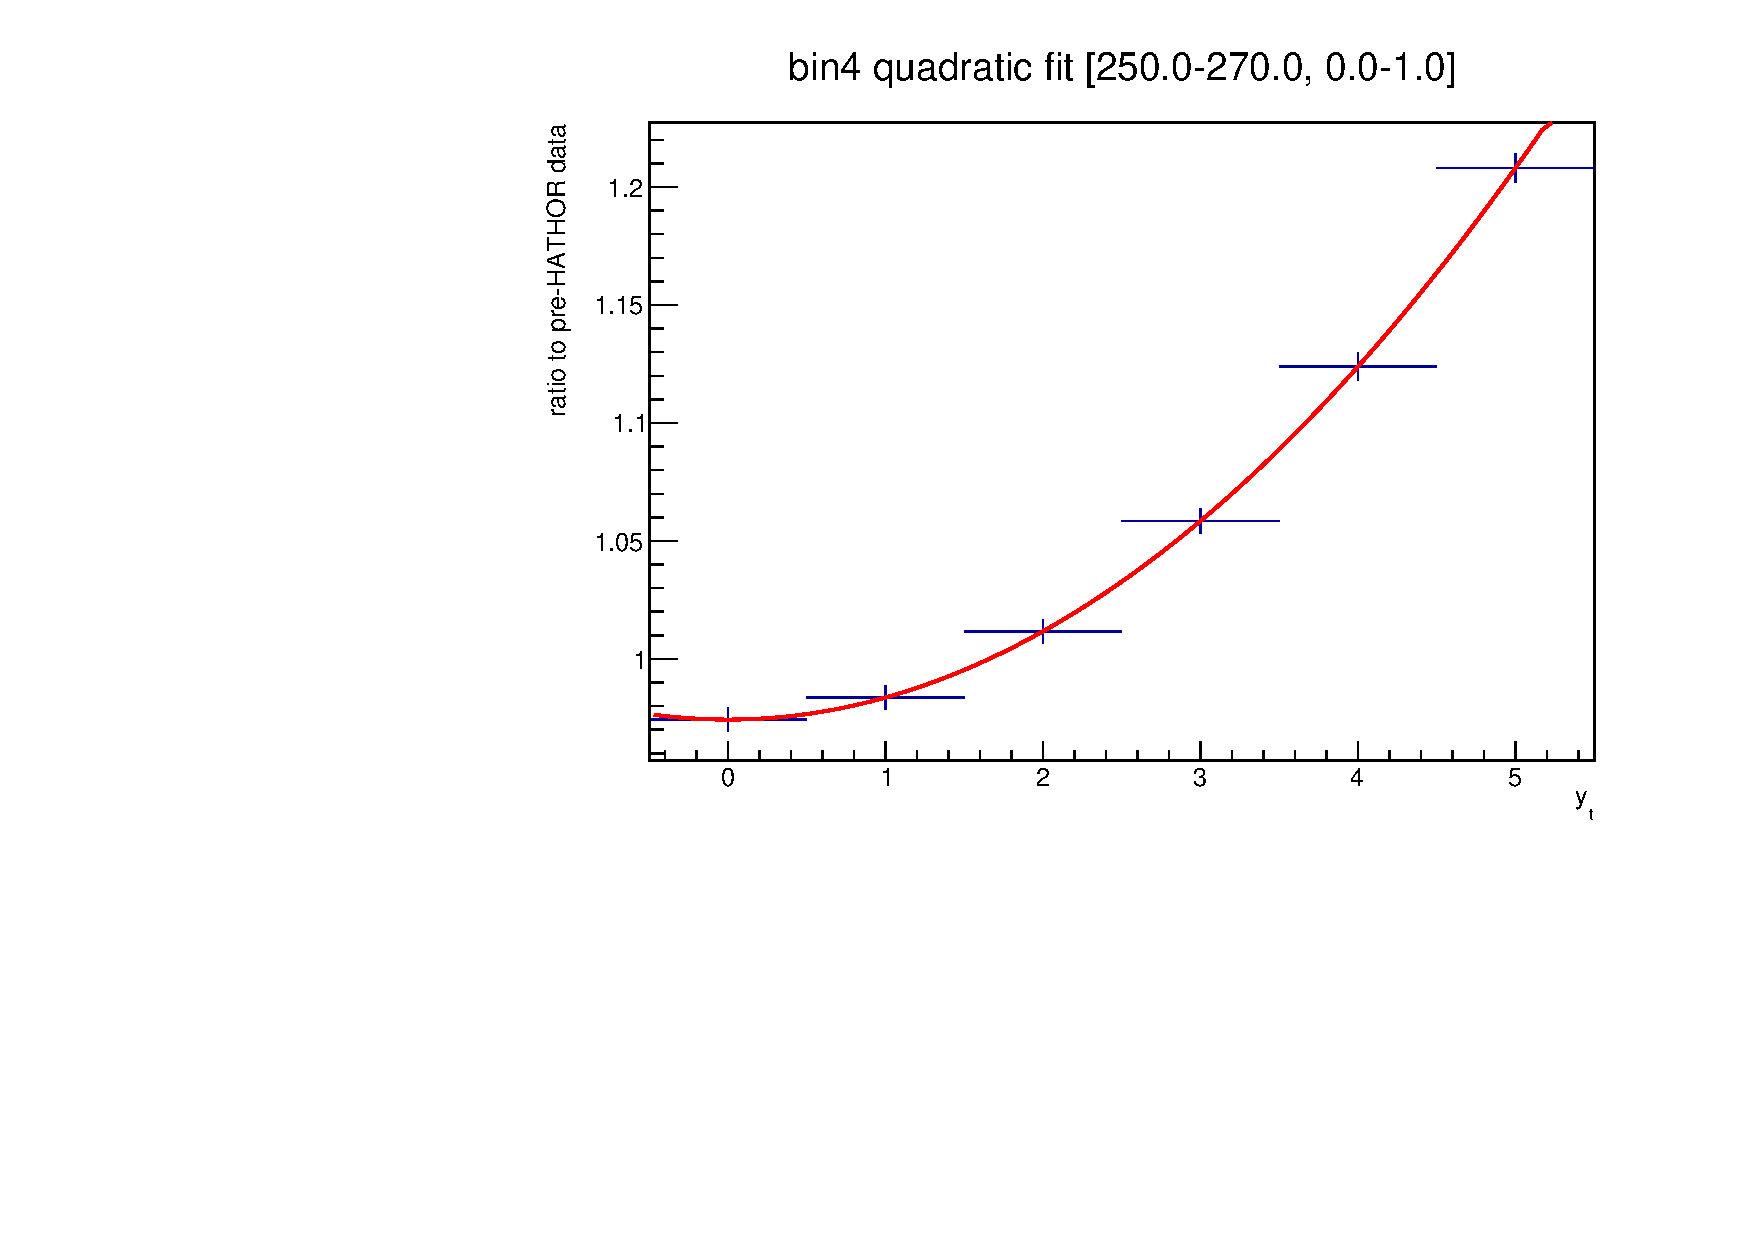
\includegraphics[width=.32\linewidth]{quadplots/2016bin4.pdf}
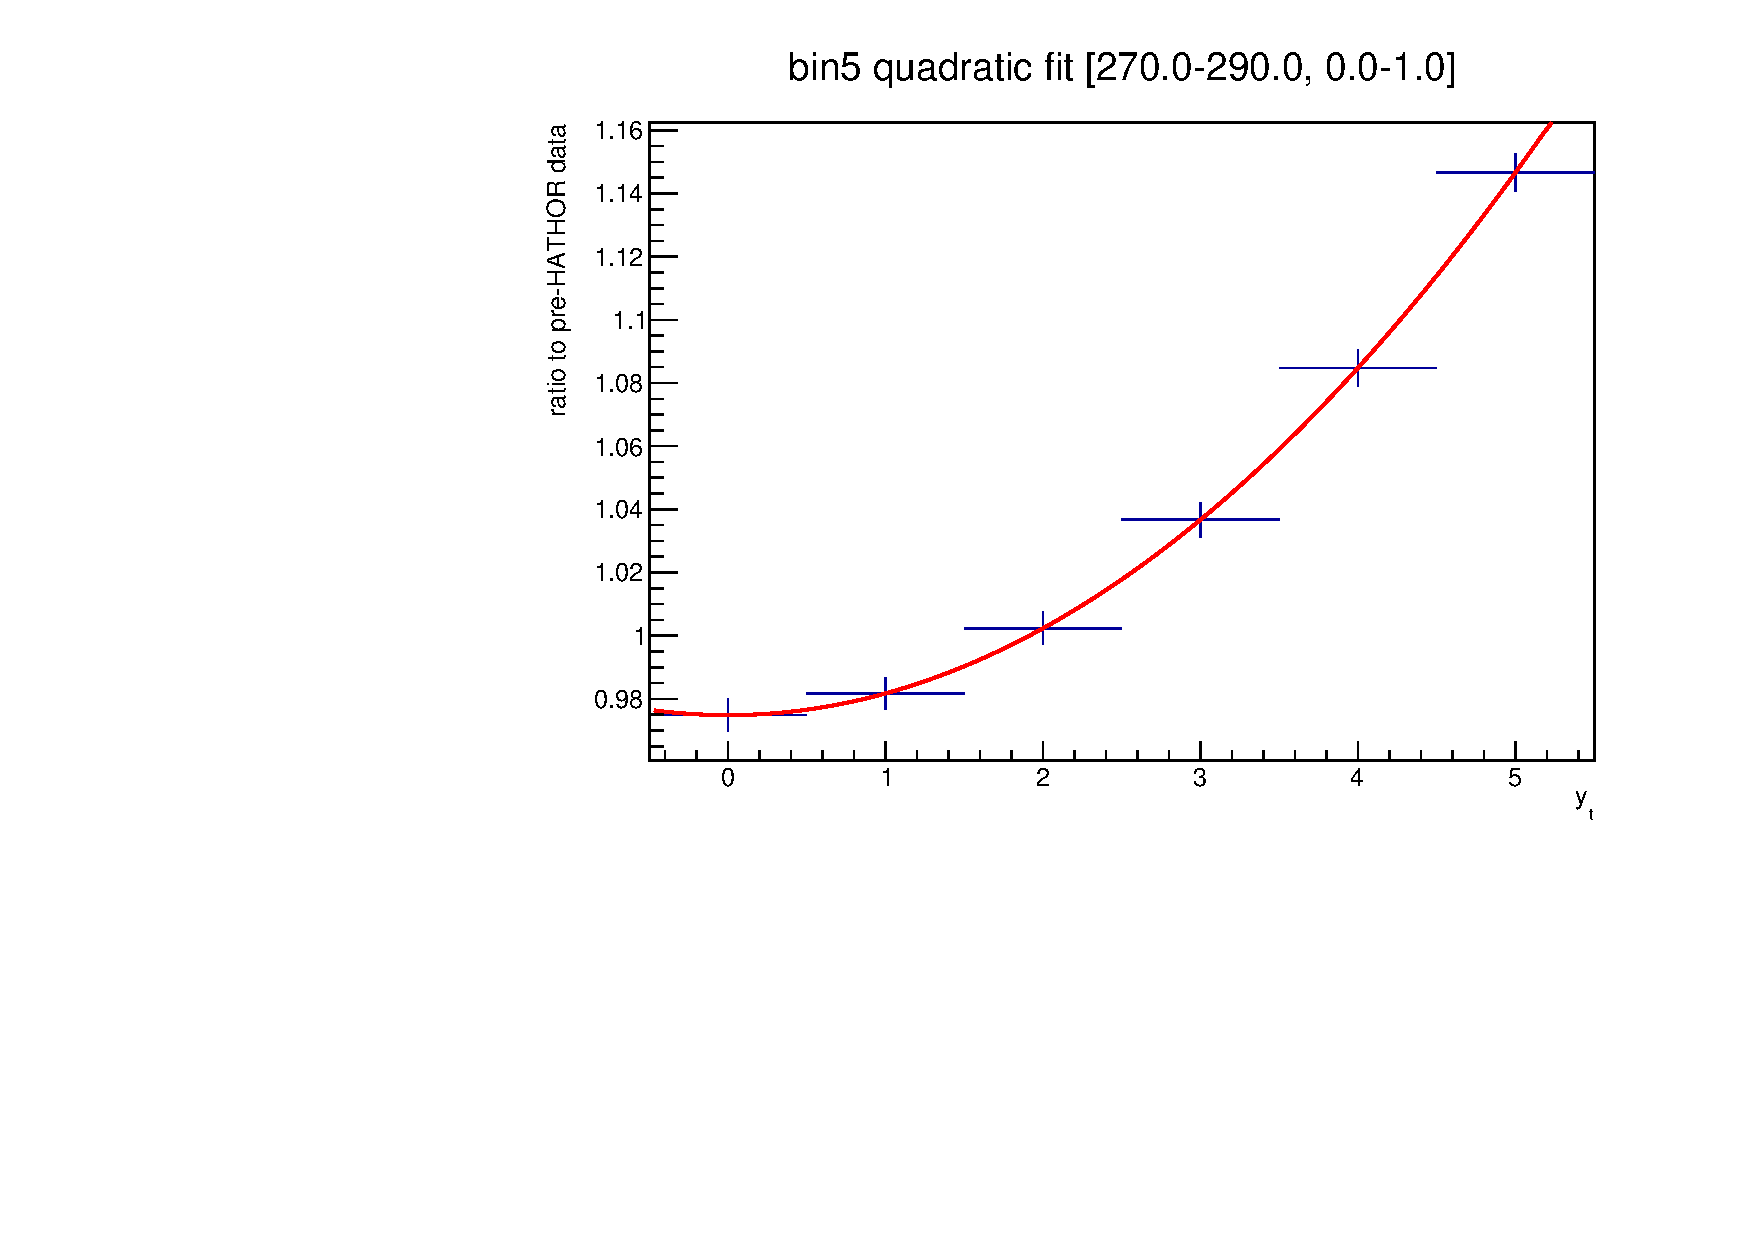
\includegraphics[width=.32\linewidth]{quadplots/2016bin5.pdf}
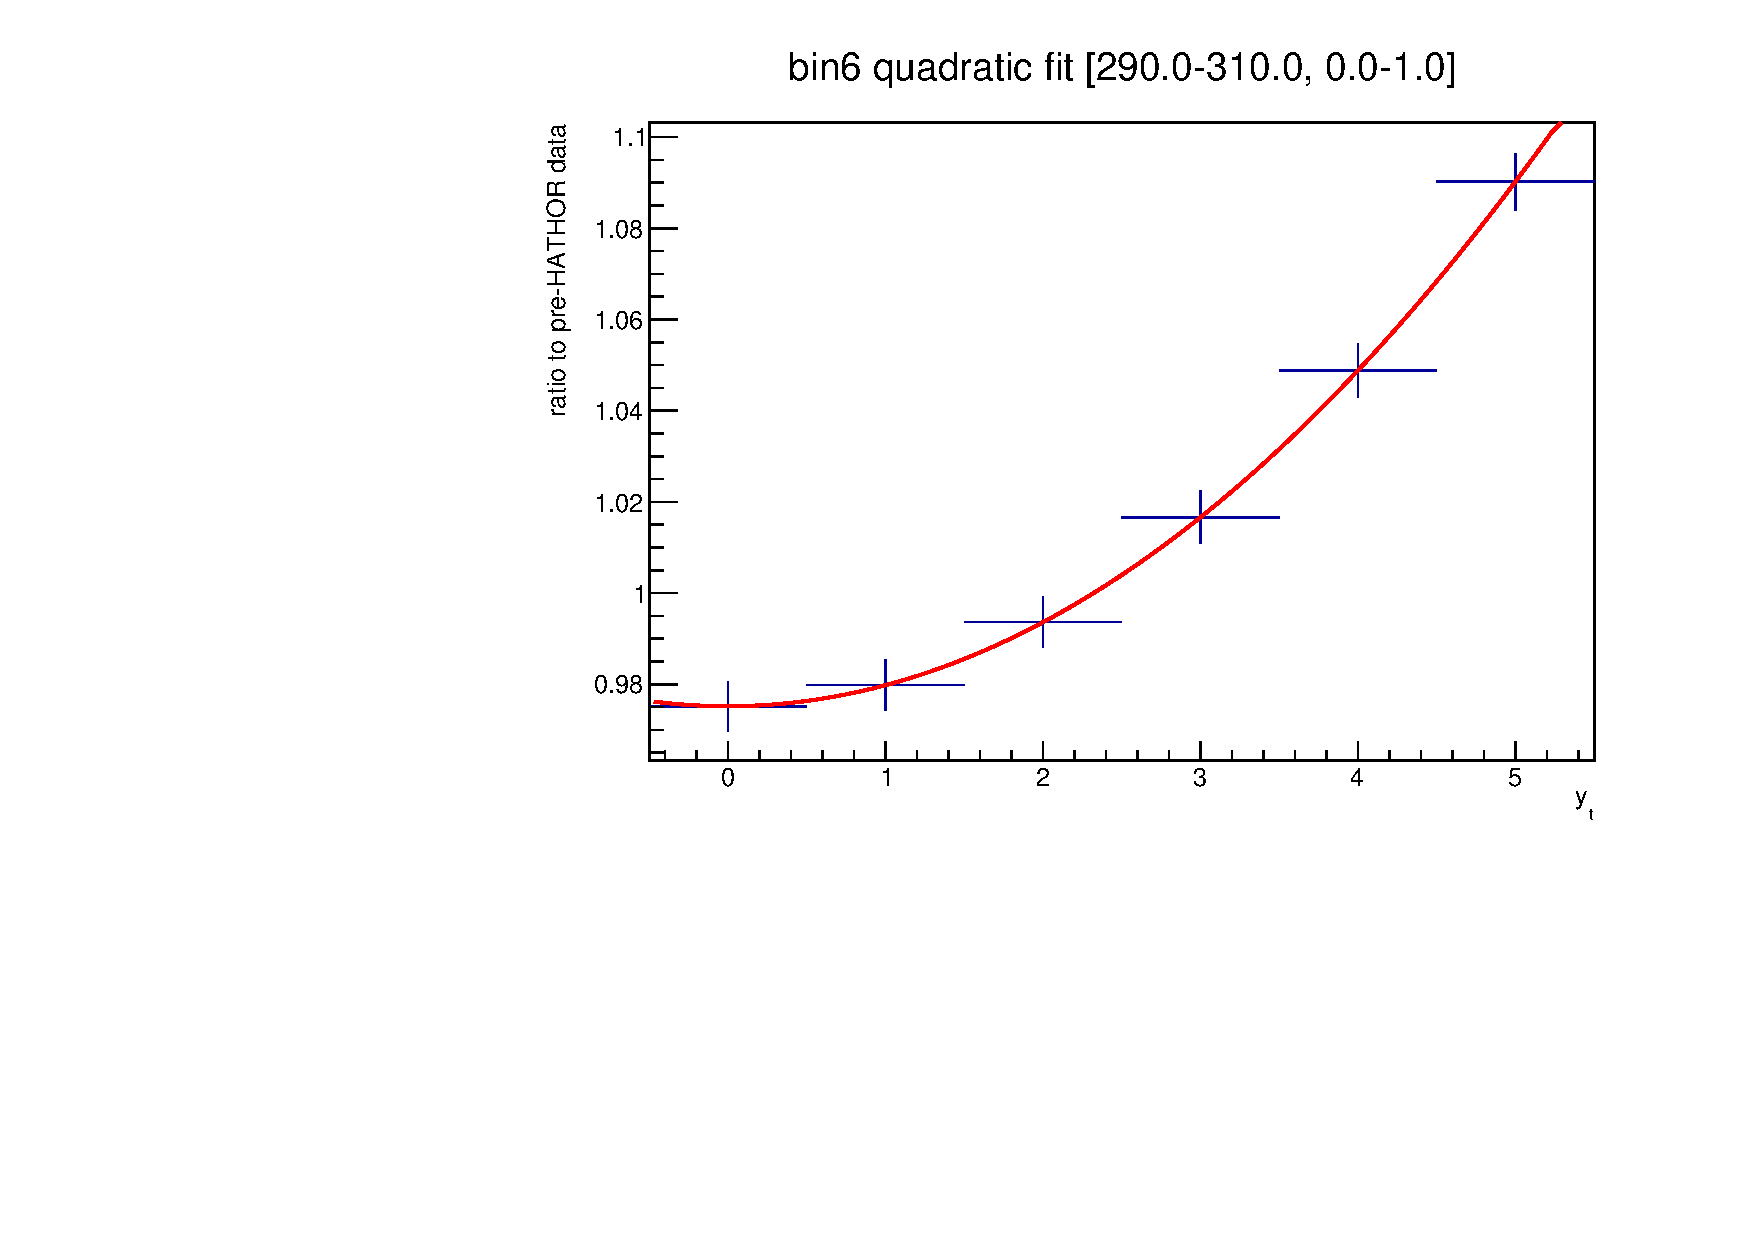
\includegraphics[width=.32\linewidth]{quadplots/2016bin6.pdf}
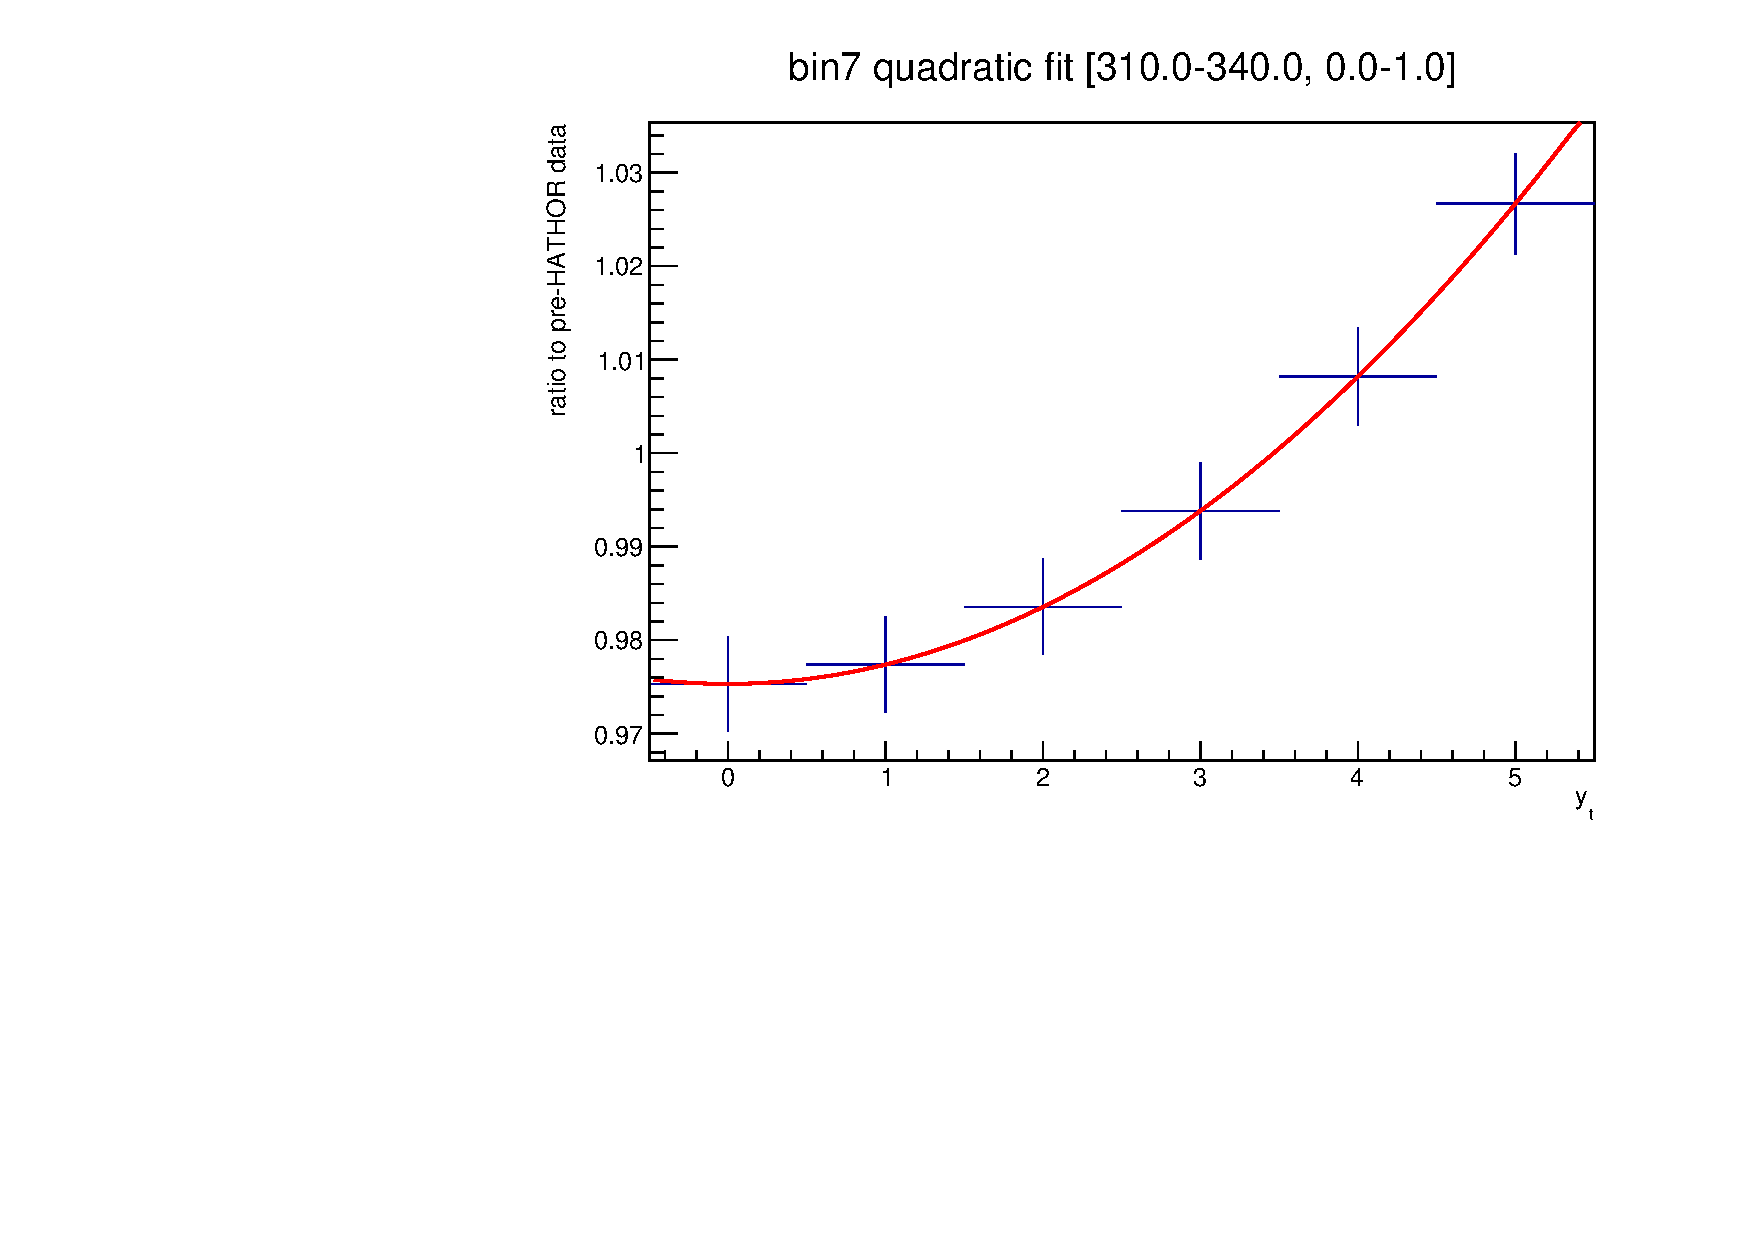
\includegraphics[width=.32\linewidth]{quadplots/2016bin7.pdf}
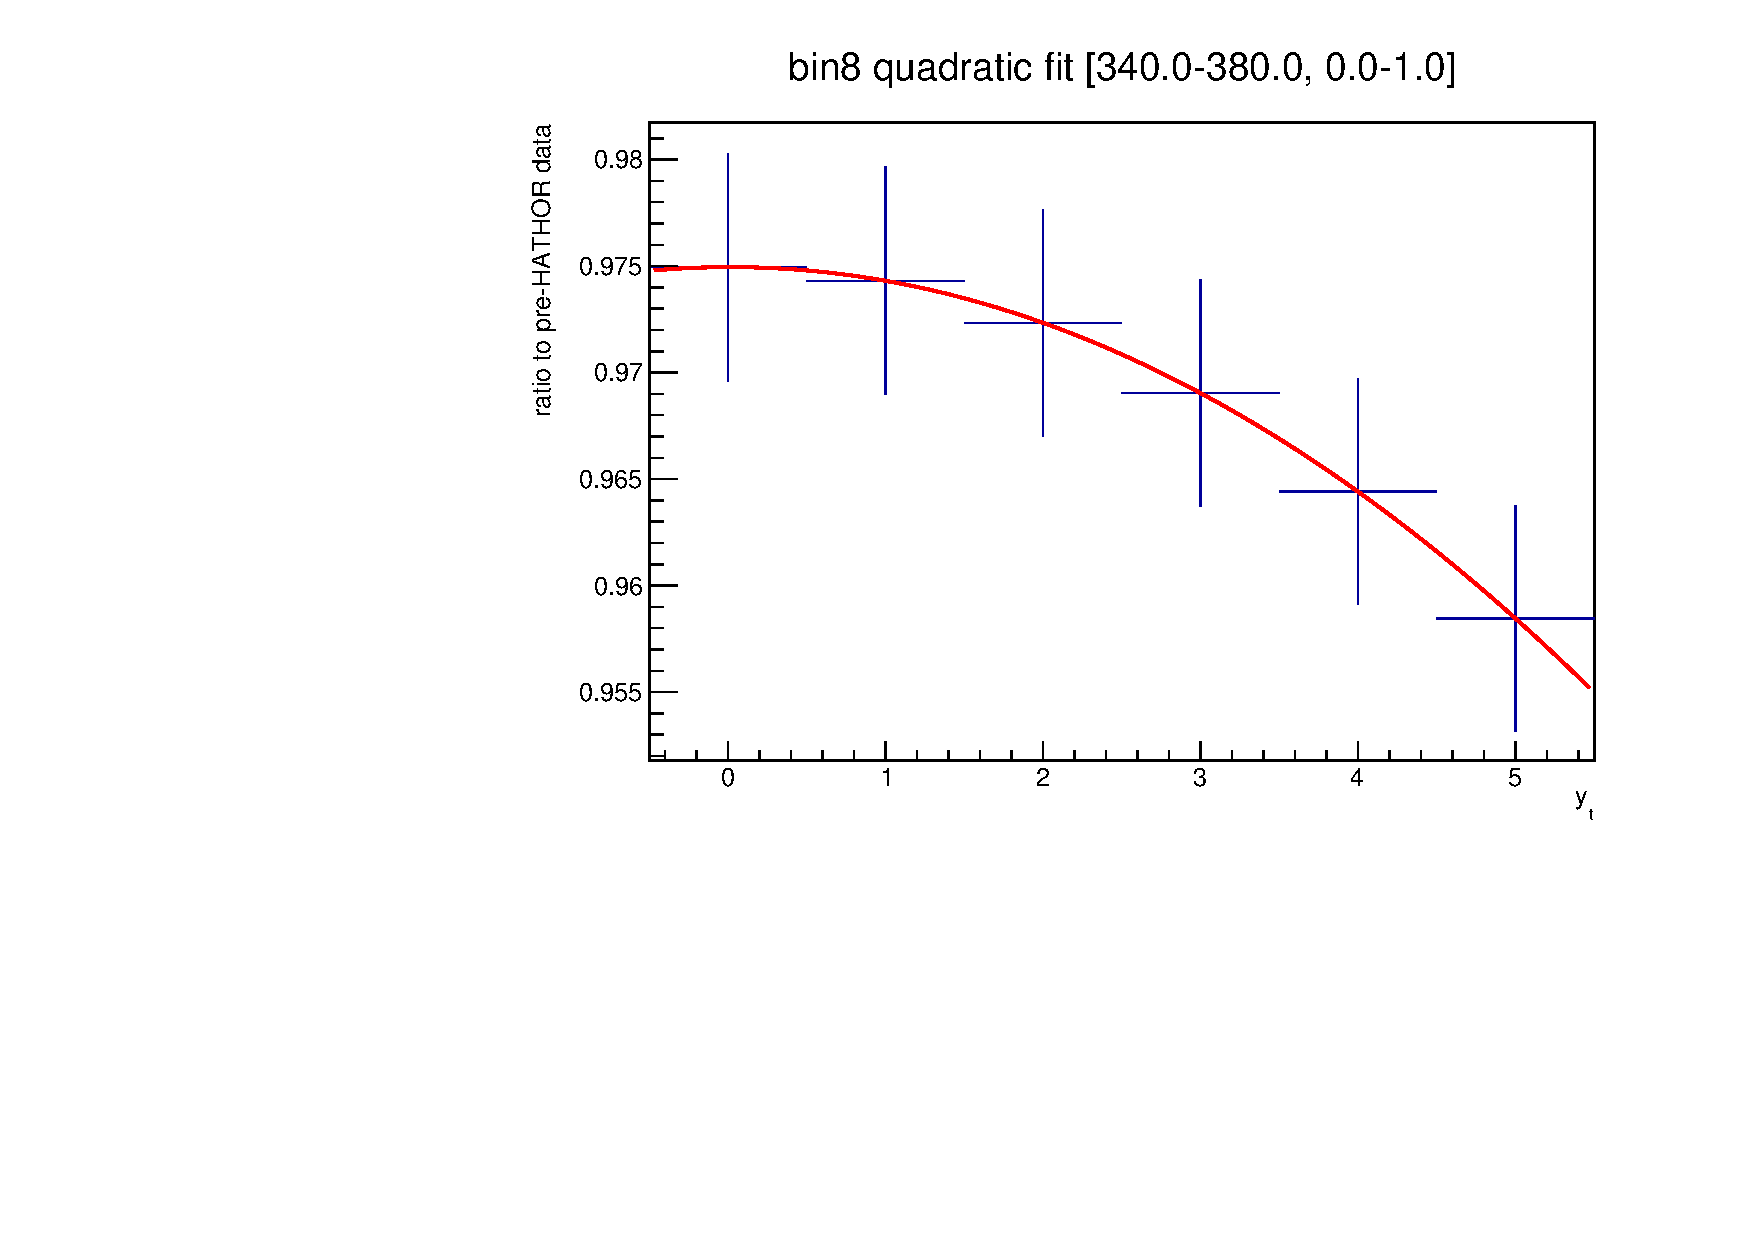
\includegraphics[width=.32\linewidth]{quadplots/2016bin8.pdf}
\includegraphics[width=.32\linewidth]{quadplots/2016bin9.pdf}
\includegraphics[width=.32\linewidth]{quadplots/2016bin10.pdf}
\includegraphics[width=.32\linewidth]{quadplots/2016bin11.pdf}
\includegraphics[width=.32\linewidth]{quadplots/2016bin12.pdf}
\includegraphics[width=.32\linewidth]{quadplots/2016bin13.pdf}
\includegraphics[width=.32\linewidth]{quadplots/2016bin14.pdf}
\includegraphics[width=.32\linewidth]{quadplots/2016bin15.pdf}
\includegraphics[width=.32\linewidth]{quadplots/2016bin16.pdf}
\includegraphics[width=.32\linewidth]{quadplots/2016bin17.pdf}
\caption{2016 bin sensitivities}
\label{fig:2016bins}
\end{figure}

\begin{figure} \centering
\includegraphics[width=.32\linewidth]{quadplots/2017bin1.pdf}
\includegraphics[width=.32\linewidth]{quadplots/2017bin2.pdf}
\includegraphics[width=.32\linewidth]{quadplots/2017bin3.pdf}
\includegraphics[width=.32\linewidth]{quadplots/2017bin4.pdf}
\includegraphics[width=.32\linewidth]{quadplots/2017bin5.pdf}
\includegraphics[width=.32\linewidth]{quadplots/2017bin6.pdf}
\includegraphics[width=.32\linewidth]{quadplots/2017bin7.pdf}
\includegraphics[width=.32\linewidth]{quadplots/2017bin8.pdf}
\includegraphics[width=.32\linewidth]{quadplots/2017bin9.pdf}
\includegraphics[width=.32\linewidth]{quadplots/2017bin10.pdf}
\includegraphics[width=.32\linewidth]{quadplots/2017bin11.pdf}
\includegraphics[width=.32\linewidth]{quadplots/2017bin12.pdf}
\includegraphics[width=.32\linewidth]{quadplots/2017bin13.pdf}
\includegraphics[width=.32\linewidth]{quadplots/2017bin14.pdf}
\includegraphics[width=.32\linewidth]{quadplots/2017bin15.pdf}
\includegraphics[width=.32\linewidth]{quadplots/2017bin16.pdf}
\includegraphics[width=.32\linewidth]{quadplots/2017bin17.pdf}
\caption{2017 bin sensitivities}
\label{fig:2017bins}
\end{figure}

\begin{figure} \centering
\includegraphics[width=.32\linewidth]{quadplots/2018bin1.pdf}
\includegraphics[width=.32\linewidth]{quadplots/2018bin2.pdf}
\includegraphics[width=.32\linewidth]{quadplots/2018bin3.pdf}
\includegraphics[width=.32\linewidth]{quadplots/2018bin4.pdf}
\includegraphics[width=.32\linewidth]{quadplots/2018bin5.pdf}
\includegraphics[width=.32\linewidth]{quadplots/2018bin6.pdf}
\includegraphics[width=.32\linewidth]{quadplots/2018bin7.pdf}
\includegraphics[width=.32\linewidth]{quadplots/2018bin8.pdf}
\includegraphics[width=.32\linewidth]{quadplots/2018bin9.pdf}
\includegraphics[width=.32\linewidth]{quadplots/2018bin10.pdf}
\includegraphics[width=.32\linewidth]{quadplots/2018bin11.pdf}
\includegraphics[width=.32\linewidth]{quadplots/2018bin12.pdf}
\includegraphics[width=.32\linewidth]{quadplots/2018bin13.pdf}
\includegraphics[width=.32\linewidth]{quadplots/2018bin14.pdf}
\includegraphics[width=.32\linewidth]{quadplots/2018bin15.pdf}
\includegraphics[width=.32\linewidth]{quadplots/2018bin16.pdf}
\includegraphics[width=.32\linewidth]{quadplots/2018bin17.pdf}
\caption{2018 bin sensitivities}
\label{fig:2018bins}
\end{figure}

\label{S:bins}
The results of the quadratic fit in \yt are shown for each analysis bin in each year

\section{Systematic template plots}
\label{S:templates}

All included systematic uncertainty templates are shown before and after pre-fit processing. The original templates are shown via shaded bars, while the smoothed templates indicated by the markers and colored lines. Red and blue indicate the up and down variations, respectively. 

During the template processing, some templates are flattened into a normalization uncertainty. These are generally very small or very noisy. They are shown below, with a flat line indicating the normalization uncertainty. Normalization uncertainties are combined into a part that is correlated between years and a part that is independent year-to-year. 

\clearpage

\begin{figure} \centering
\includegraphics[width=.35\linewidth]{templates/JES_AbsoluteMPFBias_16}\hskip-.5cm
\includegraphics[width=.35\linewidth]{templates/JES_AbsoluteMPFBias_17}\hskip-.5cm
\includegraphics[width=.35\linewidth]{templates/JES_AbsoluteMPFBias_18}
\caption{JES\_AbsoluteMPFBias templates}
\label{fig:JES-AbsoluteMPFBias_template}
\end{figure}

\begin{figure} \centering
\includegraphics[width=.35\linewidth]{templates/JES_AbsoluteScale_16}\hskip-.5cm
\includegraphics[width=.35\linewidth]{templates/JES_AbsoluteScale_17}\hskip-.5cm
\includegraphics[width=.35\linewidth]{templates/JES_AbsoluteScale_18}
\caption{JES\_AbsoluteScale templates}
\label{fig:JES-AbsoluteScale_template}
\end{figure}

\begin{figure} \centering
\includegraphics[width=.35\linewidth]{templates/JES_AbsoluteStat_16}\hskip-.5cm
\includegraphics[width=.35\linewidth]{templates/JES_AbsoluteStat_17}\hskip-.5cm
\includegraphics[width=.35\linewidth]{templates/JES_AbsoluteStat_18}
\caption{JES\_AbsoluteStat templates}
\label{fig:JES-AbsoluteStat_template}
\end{figure}

\begin{figure} \centering
\includegraphics[width=.35\linewidth]{templates/JES_FlavorQCD_16}\hskip-.5cm
\includegraphics[width=.35\linewidth]{templates/JES_FlavorQCD_17}\hskip-.5cm
\includegraphics[width=.35\linewidth]{templates/JES_FlavorQCD_18}
\caption{JES\_FlavorQCD templates}
\label{fig:JES-FlavorQCD_template}
\end{figure}

\begin{figure} \centering
\includegraphics[width=.35\linewidth]{templates/JES_Fragmentation_16}\hskip-.5cm
\includegraphics[width=.35\linewidth]{templates/JES_Fragmentation_17}\hskip-.5cm
\includegraphics[width=.35\linewidth]{templates/JES_Fragmentation_18}
\caption{JES\_Fragmentation templates}
\label{fig:JES-Fragmentation_template}
\end{figure}

\begin{figure} \centering
\includegraphics[width=.35\linewidth]{templates/JES_PileupDataMC_16}\hskip-.5cm
\includegraphics[width=.35\linewidth]{templates/JES_PileupDataMC_17}\hskip-.5cm
\includegraphics[width=.35\linewidth]{templates/JES_PileupDataMC_18}
\caption{JES\_PileupDataMC templates}
\label{fig:JES-PileupDataMC_template}
\end{figure}

\begin{figure} \centering
\includegraphics[width=.35\linewidth]{templates/JES_PileupPtBB_16}\hskip-.5cm
\includegraphics[width=.35\linewidth]{templates/JES_PileupPtBB_17}\hskip-.5cm
\includegraphics[width=.35\linewidth]{templates/JES_PileupPtBB_18}
\caption{JES\_PileupPtBB templates}
\label{fig:JES-PileupPtBB_template}
\end{figure}

\begin{figure} \centering
\includegraphics[width=.35\linewidth]{templates/JES_PileupPtEC1_16}\hskip-.5cm
\includegraphics[width=.35\linewidth]{templates/JES_PileupPtEC1_17}\hskip-.5cm
\includegraphics[width=.35\linewidth]{templates/JES_PileupPtEC1_18}
\caption{JES\_PileupPtEC1 templates}
\label{fig:JES-PileupPtEC1_template}
\end{figure}

\begin{figure} \centering
\includegraphics[width=.35\linewidth]{templates/JES_PileupPtEC2_16}\hskip-.5cm
\includegraphics[width=.35\linewidth]{templates/JES_PileupPtEC2_17}\hskip-.5cm
\includegraphics[width=.35\linewidth]{templates/JES_PileupPtEC2_18}
\caption{JES\_PileupPtEC2 templates}
\label{fig:JES-PileupPtEC2_template}
\end{figure}

\begin{figure} \centering
\includegraphics[width=.35\linewidth]{templates/JES_PileupPtHF_16}\hskip-.5cm
\includegraphics[width=.35\linewidth]{templates/JES_PileupPtHF_17}\hskip-.5cm
\includegraphics[width=.35\linewidth]{templates/JES_PileupPtHF_18}
\caption{JES\_PileupPtHF templates}
\label{fig:JES-PileupPtHF_template}
\end{figure}

\begin{figure} \centering
\includegraphics[width=.35\linewidth]{templates/JES_PileupPtRef_16}\hskip-.5cm
\includegraphics[width=.35\linewidth]{templates/JES_PileupPtRef_17}\hskip-.5cm
\includegraphics[width=.35\linewidth]{templates/JES_PileupPtRef_18}
\caption{JES\_PileupPtRef templates}
\label{fig:JES-PileupPtRef_template}
\end{figure}

\begin{figure} \centering
\includegraphics[width=.35\linewidth]{templates/JES_RelativeBal_16}\hskip-.5cm
\includegraphics[width=.35\linewidth]{templates/JES_RelativeBal_17}\hskip-.5cm
\includegraphics[width=.35\linewidth]{templates/JES_RelativeBal_18}
\caption{JES\_RelativeBal templates}
\label{fig:JES-RelativeBal_template}
\end{figure}

\begin{figure} \centering
\includegraphics[width=.35\linewidth]{templates/JES_RelativeFSR_16}\hskip-.5cm
\includegraphics[width=.35\linewidth]{templates/JES_RelativeFSR_17}\hskip-.5cm
\includegraphics[width=.35\linewidth]{templates/JES_RelativeFSR_18}
\caption{JES\_RelativeFSR templates}
\label{fig:JES-RelativeFSR_template}
\end{figure}

\begin{figure} \centering
\includegraphics[width=.35\linewidth]{templates/JES_RelativeJEREC1_16}\hskip-.5cm
\includegraphics[width=.35\linewidth]{templates/JES_RelativeJEREC1_17}\hskip-.5cm
\includegraphics[width=.35\linewidth]{templates/JES_RelativeJEREC1_18}
\caption{JES\_RelativeJEREC1 templates}
\label{fig:JES-RelativeJEREC1_template}
\end{figure}

\begin{figure} \centering
\includegraphics[width=.35\linewidth]{templates/JES_RelativeJEREC2_16}\hskip-.5cm
\includegraphics[width=.35\linewidth]{templates/JES_RelativeJEREC2_17}\hskip-.5cm
\includegraphics[width=.35\linewidth]{templates/JES_RelativeJEREC2_18}
\caption{JES\_RelativeJEREC2 templates}
\label{fig:JES-RelativeJEREC2_template}
\end{figure}

\begin{figure} \centering
\includegraphics[width=.35\linewidth]{templates/JES_RelativeJERHF_16}\hskip-.5cm
\includegraphics[width=.35\linewidth]{templates/JES_RelativeJERHF_17}\hskip-.5cm
\includegraphics[width=.35\linewidth]{templates/JES_RelativeJERHF_18}
\caption{JES\_RelativeJERHF templates}
\label{fig:JES-RelativeJERHF_template}
\end{figure}

\begin{figure} \centering
\includegraphics[width=.35\linewidth]{templates/JES_RelativePtBB_16}\hskip-.5cm
\includegraphics[width=.35\linewidth]{templates/JES_RelativePtBB_17}\hskip-.5cm
\includegraphics[width=.35\linewidth]{templates/JES_RelativePtBB_18}
\caption{JES\_RelativePtBB templates}
\label{fig:JES-RelativePtBB_template}
\end{figure}

\begin{figure} \centering
\includegraphics[width=.35\linewidth]{templates/JES_RelativePtEC1_16}\hskip-.5cm
\includegraphics[width=.35\linewidth]{templates/JES_RelativePtEC1_17}\hskip-.5cm
\includegraphics[width=.35\linewidth]{templates/JES_RelativePtEC1_18}
\caption{JES\_RelativePtEC1 templates}
\label{fig:JES-RelativePtEC1_template}
\end{figure}

\begin{figure} \centering
\includegraphics[width=.35\linewidth]{templates/JES_RelativePtEC2_16}\hskip-.5cm
\includegraphics[width=.35\linewidth]{templates/JES_RelativePtEC2_17}\hskip-.5cm
\includegraphics[width=.35\linewidth]{templates/JES_RelativePtEC2_18}
\caption{JES\_RelativePtEC2 templates}
\label{fig:JES-RelativePtEC2_template}
\end{figure}

\begin{figure} \centering
\includegraphics[width=.35\linewidth]{templates/JES_RelativePtHF_16}\hskip-.5cm
\includegraphics[width=.35\linewidth]{templates/JES_RelativePtHF_17}\hskip-.5cm
\includegraphics[width=.35\linewidth]{templates/JES_RelativePtHF_18}
\caption{JES\_RelativePtHF templates}
\label{fig:JES-RelativePtHF_template}
\end{figure}

\begin{figure} \centering
\includegraphics[width=.35\linewidth]{templates/JES_RelativeSample_16}\hskip-.5cm
\includegraphics[width=.35\linewidth]{templates/JES_RelativeSample_17}\hskip-.5cm
\includegraphics[width=.35\linewidth]{templates/JES_RelativeSample_18}
\caption{JES\_RelativeSample templates}
\label{fig:JES-RelativeSample_template}
\end{figure}

\begin{figure} \centering
\includegraphics[width=.35\linewidth]{templates/JES_SinglePionECAL_16}\hskip-.5cm
\includegraphics[width=.35\linewidth]{templates/JES_SinglePionECAL_17}\hskip-.5cm
\includegraphics[width=.35\linewidth]{templates/JES_SinglePionECAL_18}
\caption{JES\_SinglePionECAL templates}
\label{fig:JES-SinglePionECAL_template}
\end{figure}

\begin{figure} \centering
\includegraphics[width=.35\linewidth]{templates/JES_SinglePionHCAL_16}\hskip-.5cm
\includegraphics[width=.35\linewidth]{templates/JES_SinglePionHCAL_17}\hskip-.5cm
\includegraphics[width=.35\linewidth]{templates/JES_SinglePionHCAL_18}
\caption{JES\_SinglePionHCAL templates}
\label{fig:JES-SinglePionHCAL_template}
\end{figure}

\begin{figure} \centering
\includegraphics[width=.35\linewidth]{templates/JES_TimePtEta_16}\hskip-.5cm
\includegraphics[width=.35\linewidth]{templates/JES_TimePtEta_17}\hskip-.5cm
\includegraphics[width=.35\linewidth]{templates/JES_TimePtEta_18}
\caption{JES\_TimePtEta templates}
\label{fig:JES-TimePtEta_template}
\end{figure}

\begin{figure} \centering
\includegraphics[width=.35\linewidth]{templates/JERup_16}\hskip-.5cm
\includegraphics[width=.35\linewidth]{templates/JERup_17}\hskip-.5cm
\includegraphics[width=.35\linewidth]{templates/JERup_18}
\caption{JER up templates}
\label{fig:JERup_template}
\end{figure}

\begin{figure} \centering
\includegraphics[width=.35\linewidth]{templates/JERdown_16}\hskip-.5cm
\includegraphics[width=.35\linewidth]{templates/JERdown_17}\hskip-.5cm
\includegraphics[width=.35\linewidth]{templates/JERdown_18}
\caption{JER down templates}
\label{fig:JERdown_template}
\end{figure}

\begin{figure} \centering
\includegraphics[width=.35\linewidth]{templates/bdec_16}\hskip-.5cm
\includegraphics[width=.35\linewidth]{templates/bdec_17}\hskip-.5cm
\includegraphics[width=.35\linewidth]{templates/bdec_18}
\caption{bdec templates}
\label{fig:bdec_template}
\end{figure}

\begin{figure} \centering
\includegraphics[width=.35\linewidth]{templates/bfrag_16}\hskip-.5cm
\includegraphics[width=.35\linewidth]{templates/bfrag_17}\hskip-.5cm
\includegraphics[width=.35\linewidth]{templates/bfrag_18}
\caption{bfrag templates}
\label{fig:bfrag_template}
\end{figure}

\begin{figure} \centering
\includegraphics[width=.35\linewidth]{templates/btag_16}\hskip-.5cm
\includegraphics[width=.35\linewidth]{templates/btag_17}\hskip-.5cm
\includegraphics[width=.35\linewidth]{templates/btag_18}
\caption{btag templates}
\label{fig:btag_template}
\end{figure}

\begin{figure} \centering
\includegraphics[width=.35\linewidth]{templates/elrec_16}\hskip-.5cm
\includegraphics[width=.35\linewidth]{templates/elrec_17}\hskip-.5cm
\includegraphics[width=.35\linewidth]{templates/elrec_18}
\caption{elrec templates}
\label{fig:elrec_template}
\end{figure}

\begin{figure} \centering
\includegraphics[width=.35\linewidth]{templates/eltrg_16}\hskip-.5cm
\includegraphics[width=.35\linewidth]{templates/eltrg_17}\hskip-.5cm
\includegraphics[width=.35\linewidth]{templates/eltrg_18}
\caption{eltrg templates}
\label{fig:eltrg_template}
\end{figure}

% \begin{figure} \centering
% \includegraphics[width=.35\linewidth]{templates/flatsys18_16}\hskip-.5cm
% \includegraphics[width=.35\linewidth]{templates/flatsys18_17}\hskip-.5cm
% \includegraphics[width=.35\linewidth]{templates/flatsys18_18}
% \caption{flatsys18 templates}
% \label{fig:flatsys18_template}
% \end{figure}

\begin{figure} \centering
\includegraphics[width=.35\linewidth]{templates/fs_16}\hskip-.5cm
\includegraphics[width=.35\linewidth]{templates/fs_17}\hskip-.5cm
\includegraphics[width=.35\linewidth]{templates/fs_18}
\caption{fs templates}
\label{fig:fs_template}
\end{figure}

\begin{figure} \centering
\includegraphics[width=.35\linewidth]{templates/fsr_16}\hskip-.5cm
\includegraphics[width=.35\linewidth]{templates/fsr_17}\hskip-.5cm
\includegraphics[width=.35\linewidth]{templates/fsr_18}
\caption{fsr templates}
\label{fig:fsr_template}
\end{figure}

\begin{figure} \centering
\includegraphics[width=.35\linewidth]{templates/hd_16}\hskip-.5cm
\includegraphics[width=.35\linewidth]{templates/hd_17}\hskip-.5cm
\includegraphics[width=.35\linewidth]{templates/hd_18}
\caption{hd templates}
\label{fig:hd_template}
\end{figure}

\begin{figure} \centering
\includegraphics[width=.35\linewidth]{templates/isr_16}\hskip-.5cm
\includegraphics[width=.35\linewidth]{templates/isr_17}\hskip-.5cm
\includegraphics[width=.35\linewidth]{templates/isr_18}
\caption{isr templates}
\label{fig:isr_template}
\end{figure}

\begin{figure} \centering
\includegraphics[width=.35\linewidth]{templates/ltag_16}\hskip-.5cm
\includegraphics[width=.35\linewidth]{templates/ltag_17}\hskip-.5cm
\includegraphics[width=.35\linewidth]{templates/ltag_18}
\caption{ltag templates}
\label{fig:ltag_template}
\end{figure}




\begin{figure} \centering
\includegraphics[width=.32\linewidth]{templates/mtop_16_old}
\includegraphics[width=.32\linewidth]{templates/mtop_17_old}
\includegraphics[width=.32\linewidth]{templates/mtop_18_old}
\caption{mtop original templates. One can see common features, but the templates are too noisy for the smoothing to yield a reasonable shape. These are NOT included in the fit}
\label{fig:mtop_template_old}
\end{figure}

\begin{figure} \centering
\includegraphics[width=.32\linewidth]{templates/mtop_16}
\includegraphics[width=.32\linewidth]{templates/mtop_17}
\includegraphics[width=.32\linewidth]{templates/mtop_18}
\caption{mtop templates after combining all 3 years to make a single template. After combining and smoothing, we see a reasonable shape effect which captures the features shared between the 3 templates in Fig. \ref{fig:mtop_template_old}. Thus, one shape is used for all 3 years.}

\label{fig:mtop_template}
\end{figure}

\begin{figure} \centering
\includegraphics[width=.35\linewidth]{templates/murec_16}\hskip-.5cm
\includegraphics[width=.35\linewidth]{templates/murec_17}\hskip-.5cm
\includegraphics[width=.35\linewidth]{templates/murec_18}
\caption{murec templates}
\label{fig:murec_template}
\end{figure}

\begin{figure} \centering
\includegraphics[width=.35\linewidth]{templates/mutrg_16}\hskip-.5cm
\includegraphics[width=.35\linewidth]{templates/mutrg_17}\hskip-.5cm
\includegraphics[width=.35\linewidth]{templates/mutrg_18}
\caption{mutrg templates}
\label{fig:mutrg_template}
\end{figure}

\begin{figure} \centering
\includegraphics[width=.35\linewidth]{templates/pdf0_16}\hskip-.5cm
\includegraphics[width=.35\linewidth]{templates/pdf0_17}\hskip-.5cm
\includegraphics[width=.35\linewidth]{templates/pdf0_18}
\caption{pdf0 templates}
\label{fig:pdf0_template}
\end{figure}

\begin{figure} \centering
\includegraphics[width=.35\linewidth]{templates/pdf1_16}\hskip-.5cm
\includegraphics[width=.35\linewidth]{templates/pdf1_17}\hskip-.5cm
\includegraphics[width=.35\linewidth]{templates/pdf1_18}
\caption{pdf1 templates}
\label{fig:pdf1_template}
\end{figure}

\begin{figure} \centering
\includegraphics[width=.35\linewidth]{templates/pdf2_16}\hskip-.5cm
\includegraphics[width=.35\linewidth]{templates/pdf2_17}\hskip-.5cm
\includegraphics[width=.35\linewidth]{templates/pdf2_18}
\caption{pdf2 templates}
\label{fig:pdf2_template}
\end{figure}

\begin{figure} \centering
\includegraphics[width=.35\linewidth]{templates/pdf3_16}\hskip-.5cm
\includegraphics[width=.35\linewidth]{templates/pdf3_17}\hskip-.5cm
\includegraphics[width=.35\linewidth]{templates/pdf3_18}
\caption{pdf3 templates}
\label{fig:pdf3_template}
\end{figure}

\begin{figure} \centering
\includegraphics[width=.35\linewidth]{templates/pdf4_16}\hskip-.5cm
\includegraphics[width=.35\linewidth]{templates/pdf4_17}\hskip-.5cm
\includegraphics[width=.35\linewidth]{templates/pdf4_18}
\caption{pdf4 templates}
\label{fig:pdf4_template}
\end{figure}

\begin{figure} \centering
\includegraphics[width=.35\linewidth]{templates/pdf5_16}\hskip-.5cm
\includegraphics[width=.35\linewidth]{templates/pdf5_17}\hskip-.5cm
\includegraphics[width=.35\linewidth]{templates/pdf5_18}
\caption{pdf5 templates}
\label{fig:pdf5_template}
\end{figure}

\begin{figure} \centering
\includegraphics[width=.35\linewidth]{templates/pdf6_16}\hskip-.5cm
\includegraphics[width=.35\linewidth]{templates/pdf6_17}\hskip-.5cm
\includegraphics[width=.35\linewidth]{templates/pdf6_18}
\caption{pdf6 templates}
\label{fig:pdf6_template}
\end{figure}

\begin{figure} \centering
\includegraphics[width=.35\linewidth]{templates/pdf7_16}\hskip-.5cm
\includegraphics[width=.35\linewidth]{templates/pdf7_17}\hskip-.5cm
\includegraphics[width=.35\linewidth]{templates/pdf7_18}
\caption{pdf7 templates}
\label{fig:pdf7_template}
\end{figure}

\begin{figure} \centering
\includegraphics[width=.35\linewidth]{templates/pdf8_16}\hskip-.5cm
\includegraphics[width=.35\linewidth]{templates/pdf8_17}\hskip-.5cm
\includegraphics[width=.35\linewidth]{templates/pdf8_18}
\caption{pdf8 templates}
\label{fig:pdf8_template}
\end{figure}

\begin{figure} \centering
\includegraphics[width=.35\linewidth]{templates/pdf9_16}\hskip-.5cm
\includegraphics[width=.35\linewidth]{templates/pdf9_17}\hskip-.5cm
\includegraphics[width=.35\linewidth]{templates/pdf9_18}
\caption{pdf9 templates}
\label{fig:pdf9_template}
\end{figure}


\begin{figure} \centering
\includegraphics[width=.35\linewidth]{templates/pdf_as_16}\hskip-.5cm
\includegraphics[width=.35\linewidth]{templates/pdf_as_17}\hskip-.5cm
\includegraphics[width=.35\linewidth]{templates/pdf_as_18}
\caption{pdf-as template }
\label{fig:pdfas_template}
\end{figure}


\clearpage



\begin{figure} \centering
\includegraphics[width=.35\linewidth]{templates/pu_16}\hskip-.5cm
\includegraphics[width=.35\linewidth]{templates/pu_17}\hskip-.5cm
\includegraphics[width=.35\linewidth]{templates/pu_18}
\caption{pu templates}
\label{fig:pu_template}
\end{figure}

\begin{figure} \centering
\includegraphics[width=.35\linewidth]{templates/rs_16}\hskip-.5cm
\includegraphics[width=.35\linewidth]{templates/rs_17}\hskip-.5cm
\includegraphics[width=.35\linewidth]{templates/rs_18}
\caption{rs templates}
\label{fig:rs_template}
\end{figure}

\begin{figure} \centering
\includegraphics[width=.35\linewidth]{templates/rsfs_16}\hskip-.5cm
\includegraphics[width=.35\linewidth]{templates/rsfs_17}\hskip-.5cm
\includegraphics[width=.35\linewidth]{templates/rsfs_18}
\caption{rsfs templates}
\label{fig:rsfs_template}
\end{figure}





\begin{figure} \centering
\includegraphics[width=.35\linewidth]{templates/tune_16}\hskip-.5cm
\includegraphics[width=.35\linewidth]{templates/tune_17}\hskip-.5cm
\includegraphics[width=.35\linewidth]{templates/tune_18}
\caption{tune templates}
\label{fig:tune_template}
\end{figure}


\clearpage

\section{Additional Impacts}
The full 3 pages of systematic uncertainty impacts from the sensitivity study are shown here
\label{S:fullimpacts}

    \centering
    \includegraphics[width=.8\linewidth]{figs/impacts1.pdf}

    \centering
    \includegraphics[width=.8\linewidth]{figs/impacts2.pdf}

    \centering
    \includegraphics[width=.8\linewidth]{figs/impacts3.pdf}



